\documentclass{ucbthesis}
\usepackage[backend=bibtex]{biblatex}
\bibliography{thesis}

\usepackage{times}
% \usepackage{pxfonts}

\usepackage[T1]{fontenc}
\usepackage[font=small,labelfont=bf]{caption}
\usepackage{amsmath}
\usepackage{amssymb}
\usepackage{booktabs} % For formal tables
\usepackage{caption}
\usepackage{csquotes}
\usepackage{enumitem}
\usepackage{graphicx}
\usepackage{hyperref}
\usepackage{listings}
\usepackage{mhchem}
\usepackage{microtype}
\usepackage{multirow}
\usepackage{pgfplots}
\usepackage{siunitx}
\usepackage{subcaption}
\usepackage{subfiles}
\usepackage{tablefootnote}
\usepackage{textcomp}
\usepackage{tikz}
\usepackage{xcolor}

%%%%%%%%%%%%%%%%%%%%%%%%%%%%%%%%%%%%%%%%%%%%%%%%%%%%%%%%%%%%%%%
%% Custom Styling
%%%%%%%%%%%%%%%%%%%%%%%%%%%%%%%%%%%%%%%%%%%%%%%%%%%%%%%%%%%%%%%

%% Make quote using italics
\renewcommand{\mkbegdispquote}[2]{\itshape}

%% Tune paragraph skip to look just a bit nicer!
\setlength{\parskip}{5pt}

%% French spacing inserts spaces around most punctuation marks, but
%% single-spaced after sentences, colons, and semicolons.
\frenchspacing

%% Colors stolen from acmart template
\definecolor[named]{ACMBlue}{cmyk}{1,0.1,0,0.1}
\definecolor[named]{ACMYellow}{cmyk}{0,0.16,1,0}
\definecolor[named]{ACMOrange}{cmyk}{0,0.42,1,0.01}
\definecolor[named]{ACMRed}{cmyk}{0,0.90,0.86,0}
\definecolor[named]{ACMLightBlue}{cmyk}{0.49,0.01,0,0}
\definecolor[named]{ACMGreen}{cmyk}{0.20,0,1,0.19}
\definecolor[named]{ACMPurple}{cmyk}{0.55,1,0,0.15}
\definecolor[named]{ACMDarkBlue}{cmyk}{1,0.58,0,0.21}

\hypersetup{colorlinks,
  linkcolor=ACMBlue,
  citecolor=ACMPurple,
  urlcolor=ACMDarkBlue,
  filecolor=ACMDarkBlue
}

%%%%%%%%%%%%%%%%%%%%%%%%%%%%%%%%%%%%%%%%%%%%%%%%%%%%%%%%%%%%%%%
%% Paper setup
%%%%%%%%%%%%%%%%%%%%%%%%%%%%%%%%%%%%%%%%%%%%%%%%%%%%%%%%%%%%%%%

\captionsetup[subfigure]{justification=justified, singlelinecheck=true}
\captionsetup[figure]{skip=10pt}

\lstset{
  captionpos=b,
  showspaces=false,
  showtabs=false,
  breaklines=true,
  showstringspaces=false,
  breakatwhitespace=true,
  escapeinside={(*@}{@*)},
  basicstyle=\footnotesize\ttfamily,
  columns=fullflexible,
  morekeywords={maybe_downsample, maybe_skip, maybe}
}

\renewcommand{\lstlistingname}{Example}

\setcounter{tocdepth}{2}
\setcounter{secnumdepth}{2}

\newcommand{\question}[1]{``\textit{#1}''}

\newcommand{\awstream}{AWStream}
\newcommand{\sysname}{AWStream}
\newcommand{\brt}{BRT}
\newcommand{\para}[1]{\smallskip\noindent\textbf{#1}}
\newcommand{\paraf}[1]{\noindent\textbf{#1}}
\newcommand{\todo}[1]{{\color{ACMRed}\textbf{TODO: #1}\normalfont}}
\newcommand{\fixme}[1]{{\color{ACMRed}\textbf{FIXME: #1}\normalfont}}

\newcommand{\maybe}{\texttt{maybe}}

\def\Snospace~{\S{}}
\renewcommand*\sectionautorefname{\Snospace}
\renewcommand*\subsectionautorefname{\Snospace}
\renewcommand*\subsubsectionautorefname{\Snospace}
\renewcommand*{\equationautorefname}{Eq.}
\renewcommand*{\figureautorefname}{Fig.}

\newcommand{\specialcell}[2][c]{%
  \begin{tabular}[#1]{@{}c@{}}#2\end{tabular}}

\newcommand*\circled[1]{\tikz[baseline=(char.base)]{
    \node[shape=circle,draw,inner sep=0.5pt] (char) {#1};}}

\newcommand*\qe{$\text{Q}_\text{E}$}
\newcommand*\qc{$\text{Q}_\text{C}$}
\newcommand*\rc{$\text{R}_\text{C}$}
\newcommand*\spd{$\text{S}_\text{ProbeDone}$}

%%% Local Variables:
%%% mode: latex
%%% TeX-master: "thesis"
%%% End:


\hypersetup{
  pdfinfo={
    Title={Adapting Swarm Applications: A Systematic and Quantitative Applications},
    Author={Ben Zhang},
    Subject={Computer Science}
  }
}

\begin{document}

\title{Adapting Swarm Applications: A Systematic and Quantitative Approach}
\author{Ben Zhang}
\degreesemester{Spring}
\degreeyear{2018}
\degree{Doctor of Philosophy}
\chair{Professor John Wawrzynek}
\othermembers{Professor Edward A. Lee \\
  Professor John Chuang \\
  Professor Sylvia Ratnasamy}
\numberofmembers{3}
\field{Computer Science}
\campus{Berkeley}

\maketitle
\approvalpage

{ \dsp\copyrightpage }

\begin{abstract}

  The growing number of Internet-connected devices (sensors and actuators) over
  the wide-area are challenging how we construct analytical
  applications. Traditional approaches separate data collection, transportation
  and distillation as individual one-shot tasks, often performed offline. They
  are a poor match to the need of acting on data in real time. Recently, the
  recognition of timely decision-making has spawned many stream processing
  systems for ``big data.''  However, these systems are primarily tailored
  towards the infrastructure within a single cluster. In a cluster, while
  resource allocation is challenging, there are usually enough resources and the
  allocation is a management problem for maximal utilization. In contrast, the
  wide-area faces resource scarcity and variability, making it not possible to
  guarantee enough allocation for applications. Instead, applications have to
  adapt their behaviors to match the available resources.

  While developers can design each individual application to match a specific
  resource configuration, the ad-hoc solution does not generalize across
  applications and different data distributions. Besides, optimizations created
  at design time often don't take the dynamics of the environment into
  consideration and will behave sub-optimally at runtime.

  Recognizing the need for an adaptive behavior across diverse wide-area
  streaming applications, this manuscript proposes a system-level approach that
  separates the application logic from adaptation mechanisms. To achieve this
  goal, I propose a three-stage design framework: (i) a high-level programming
  abstraction that allows developers to express adaptation options; (ii) an
  offline profiling tool that learns the resource demand and the impact on
  application utilities for a specific adaptation strategy---generating an
  application profile; (iii) a runtime system responsive to environment changes,
  maximizing application utility according to the learned profile.

  %% data acquisition devices running on battery have a limited energy budget;
  %% data transportation links such as wireless channels or the wide-area have
  %% limited capacity.

  The resource and adaptation above are intentionally not specific as it
  provides a general framework applicable to network resources, computing
  resources, as well as storage resources. In this proposal, I focus on the
  adaptation with regards to network resources in the wide-area. Adapting to the
  heterogeneous computing infrastructures is planned as future work. It will be
  another part of the final thesis. There is an ongoing research effort (led by
  my colleagues and I had participated) on storage resources; the final thesis
  will also briefly discuss the design and some preliminary results.

  The bulk body of this proposal focuses on network resources. Specifically, I
  present \sysname{}, a stream processing system for the wide area where the
  network capacity is scarce and variable. The key observation is the explicit
  trade-off between application accuracy and bandwidth demand. The system design
  follows the three-stage framework above: degradation APIs, offline profiling
  and a runtime system.

  Using \sysname{}, I have built three real-world applications: a pedestrian
  detection surveillance application, augmented reality for mobile devices and a
  distributed top-k. At places where traditional non-adaptive approaches would
  lead to either significant application accuracy drop or long tail latency,
  \sysname{} gracefully adapts to the network changes, maintaining the balance
  between application utility and system performance.

\end{abstract}

%%% Local Variables:
%%% mode: latex
%%% TeX-master: "thesis"
%%% End:


\begin{frontmatter}
  \begin{dedication}
    \null\vfil
    \begin{center}
      \vspace*{\fill}
      To my parents
      \vspace*{\fill}
    \end{center}
    \vfil\null
  \end{dedication}

  \tableofcontents
  \clearpage
  \listoffigures
  \clearpage
  \listoftables

  \begin{acknowledgements}
    Acknowledgment.
  \end{acknowledgements}
\end{frontmatter}

\pagestyle{headings}

\chapter{Introduction}

Wide-area streaming analytics are becoming pervasive, especially with the
emerging Internet-of-Thing (IoT) applications. Large cities such as New York,
Beijing and Seattle are deploying millions of cameras for traffic
control~\cite{london.surveillance,skynet}. Retails stores and critical areas
such as railway stations are also being monitored for abnormal
activities. Buildings are increasingly instrumented with a wide variety of
sensors to improve building energy use, occupant comfort, reliability and
maintenance~\cite{krioukov2012building}. Geo-distributed infrastructure, such as
Content Delivery Network (CDN), needs to analyze user requests (machine logs)
and optimize data placement to improve delivery efficiency. In these problems,
the data collected at the edge needs to be transported acoross the wide-area and
analyzed in real-time.

Existing stream processing for ``big data,'' such as
Storm~\cite{toshniwal2014storm} or Spark
Streaming~\cite{zaharia2013discretized}, only work in the context of a single
cluster, where the bandwidth is sufficient (or at least easy to
provision). While they are the perfect back end for analyzing streams once data
arrive, in the wide-area, the network, with scarce and variable bandwidth,
easily becomes the bottleneck \cite{rabkin2014aggregation}. What's worse, the
growth rate of wide-area network capacity is not keeping up with the increasing
rate of traffic~\cite{cisco2013zettabyte}.

When facing situations where the bandwidth is not sufficient, applications
deployed today either choose a conservative setting (e.g.\,only delivering 360p
videos) or leave their fate to the underlying transport layer: (1) in the case
of TCP, the sender will be blocked and data are backlogged, leading to severe
delay; (2) in the case of UDP, uncontrolled packet loss occurs, leading to
application performance drop. Instead of ``suffering'' from a degraded network,
applications can act proactively by adjusting their behavior: reducing the data
rate to ensure that important data are delivered in time.

The idea of adapting data rate for data freshness is not new. Multimedia
applications and their adaptations~\cite{michalos2012dynamic,
  schulzrinne1998real} have been extensively studied in the past because their
high demands on the network are rarely met. However, since their goal is to
improve \textbf{user experience}, their adaptation strategies are not
necessarily optimal for streaming analytics. For example, humans can tolerate
loss on video frame details but expect a smooth frame transition---at least 25
frames per second (FPS). But many vision analytics are based on algorithms that
extract edge information from a frame---they will perform poorly if frame
details are lost after an aggressive quantization.

The observation that different applications demand different strategies in order
to achieve the optimal adaptation calls for a system-level approach. In this
proposal, I present the design and implementation of \sysname{}, an adaptive
stream processing system for the wide-area. Under normal operations, \sysname{}
applications work with maximal data fidelity; when the network's capacity
changes, applications will react by controlling the level of
\textbf{degradation}: trading data fidelity for freshness.

Although the basic idea behind degradation is intuitive, realizing them in
practice is non-trivial. Firstly, as has been discussed earlier, different
degradations have different impacts across applications and data
distributions. Secondly, each degradation is often more than a binary decision;
they can be parameterized with a wide range of tuning space. It's not always
possible to derive a close-form analytical relationship between the degradation
parameter and its impact on the bandwidth and accuracy. What's more, real-world
applications often have multiple dimensions to tune---prohibiting a manual
exploration of all the design space. Take video analytics as an example,
reducing image resolution, frame rate or changing the video encoding quality are
all possible degradation operations. Each operation will affect data rate and
application accuracy but its impact to the video quality is not immediately
obvious for developers. The situation is worse when multiple degradations are
employed. These challenges are elaborated in~\autoref{sec:challenges}.

To address the challenges, \sysname{} employs a data-driven empirical-analysis
approach that's analogous to machine learning.  First, \sysname{} separates
application logic from adaptation strategies by providing a clean abstraction
(\texttt{maybe} APIs) for developers: this allows expressibility without
burdening the developers for an exact strategy. \sysname{} then profiles the
application using representative datasets and application-specific utility
functions to ``learn'' the optimal strategies under different network
conditions. The profile is then used to guide the runtime adaptation, for which
\sysname{} provides all the necessary ``plumbing'' modules to without
application developers' effort. In \autoref{sec:architecture}, I will present a
detailed description of \sysname{}'s architecture.

To study and validate the effect of degradation, I've built a prototype
framework and three real-world applications using \sysname{}: a street
surveillance application performing pedestrian detection, an augmented reality
application recognizing everyday objects and a distributed top-k application
analyzing web server access logs. The first two video streaming applications
have three degradation operations: reducing resolution, frame rate and video
encoding quality. For the distributed top-k application, two degradation
operations are envolved: N in a local top-N operation and T as a local
threshold. \autoref{sec:build-appl} discusses the considerations and details
about the prototype.

The evaluation shows that the offline profiling is able to explore the design
space for all three applications and generate the Pareto-optimal adaptation
strategies that was not achievable with manual developer configurations or with
only a single degradation operation. These profiles offer a quantitative
understanding of each application's behavior. During runtime, \sysname{}
applications are compared against traditional transport protocols including TCP
and UDP with a controlled experiment. When the network capacity drops, TCP
creates a severe delay; and the delay increases linearly as time goes; for UDP,
a severe packet loss makes the application unusable. Applications built with
\sysname{} handles the network variation gracefully: video streaming analytics
is able to keep the latency bounded with 2 seconds and the accuracy higher than
80\%. For the top-k application, although the feedback is less frequent and
adaptation is not always immediate, the worst-case latency is 12 seconds at most
and the accuracy is mostly above 75\%.

To this end, this thesis makes the following contributions:

\begin{itemize}
\item An in-depth study of wide-area streaming applications in the case of
  network resource variation.
\item The proposal of novel APIs to allow for a design space exploration between
  bandwidth and accuracy with minimal developer effort.
\item A prototype implementation that demonstrates application profiling and
  runtime adaptation.
\item Thorough evaluations based on three real-world applications under
  different scenarios.
\end{itemize}

\section{Motivating Applications}
\label{sec:motiv-appl}

There is a variety of wide-area streaing applications. We discuss three
applications with their implications.

\para{Video Surveillance:} We envisage a city-wide monitoring system that
aggregates camera feeds (both stationary ground cameras and moving aerial
vehicles) and analyzes video streams in real-time for surveillance, anomaly
detection or business intelligence~\cite{oh2011large}. While traditionally human
labors are involved in analyzing abnormal activities, recent advances in
computer vision and deep learning has dramatically increased the accuracy for
automatic analysis of visual scenes, such as pedestrian
detection~\cite{dollar2012pedestrian}, vehicle tracking~\cite{coifman1998real},
or facial recognition to locate people of
interest~\cite{Lu:2015:SHF:2888116.2888245, parkhi2015deep}.
% \cite{gantz2012digital}

\para{Electrical Grid Monitoring:} While traditional environmental sensors are
slow~\cite{atzori2010internet}, we are seeing an increasing trend with
high-frequency, high-precision sensors being deployed. For example, the
microsynchophasors monitoring system for the electrical grid consists of a
network of 1000 devices; each produces 12 streams of 120 Hz high-precision
values accurate to 100 ns. This amounts to 1.4 million points per second that
requires specialized timeseries database~\cite{andersen2016btrdb}.

\para{Log Analysis:} Large organizations today are managing 10--100s of
datacenters (DCs) and edge clusters worldwide~\cite{calder2013mapping}. While
most log analysis today runs in a batch mode and at most on a daily basis, there
is a trend in analyzing logs in real time for quicker
optimization~\cite{alspaugh2014analyzing}. For example, by analyzing the access
logs in real time, a content distribution network (CDN) can improve the overall
delivery efficiency with optimized data placement.

\vspace{0.5em}

These applications share a similar structure: a large volume of data generated
at the edge need to be transported across the wide area network for real time
analysis. Because of the limited network resources in the wide area, they will
face practical issues when deployed at a scale.

\section{Wide-Area Bandwidth Characteristics}
\label{sec:making-case-adapt}

\begin{figure}
  \centering
  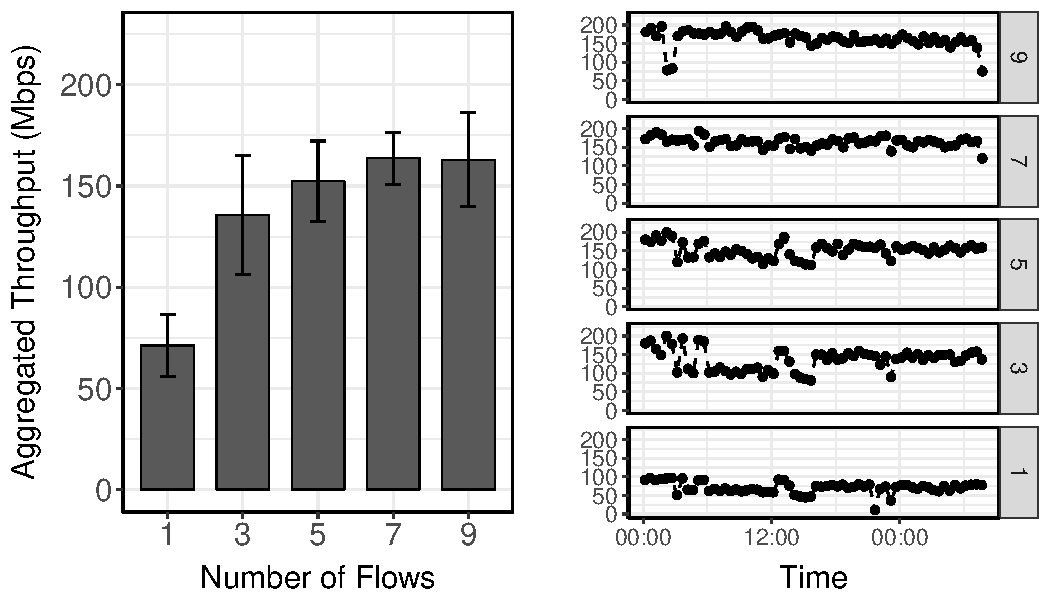
\includegraphics[width=.95\linewidth]{figures/europe-to-us-west.pdf}
  \caption{Bandwidth measurement between Amazon EC2 sites (from Ireland to
    California). Note the time-series plot has a resolution of 30 minutes; each
    point is more than a short period of transient degradation.}
  \label{fig:bw}
\end{figure}

To understand the bandwidth characteristics in the wide-area, I conducted a
simple measurement using Amazon EC2. iPerf~\cite{iperf} was used to measure the
pair-wise bandwidth between four geo-distributed sites throughout the day. The
measurement shows large variance in the measured bandwidth and one such pair of
sites is shown in \autoref{fig:bw}. Regardless of the number of
flows\footnote{EC2 has a per-flow and per-VM rate
  limiting~\cite{zhang2016guaranteeing}.}, there exist occasions when the
available bandwidth is almost halved. Generally speaking, the back-haul links
between EC2 sites are better (if not at least representative) in comparison to
the overall wide-area link quality. This varying nature poses real challenges to
the realization and successful deployment of wide-area streaming applications.

\section{Making the Case for a System Approach}
\label{sec:bat}

When facing insufficient network bandwidth, applications that do not adapt will
suffer severe performance penalty: such as a backlog of data for TCP or
uncontrolled packet loss for UDP. Instead of giving up control to the underlying
transport layer, applications can react and adapt their behaivors to the
resource changes.

While adaptive streaming exists in certain application domains, there has not
been a general solution. Consider video streaming applications that have been
extensively studied in the literature. There are a plethora of encoding
techniques~\cite{richardson2011h, grange2016vp9} with adaptive
strategies~\cite{yin2015control, michalos2012dynamic, pantos2016http}, however,
their primary goal is to optimize end-user quality of experience (QoE).  When
end users consume a video clip, a smooth video is often more enjoyable than
videos with intermittent pauses, even though each pause has crisp images.

Optimizing for QoE doesn't work for our target applications. Each video
analytics has its own goal, entailing different adaptive strategies for
different applications. For example, some computer vision detection algorithms
rely on the edge information~\cite{canny1986computational, lowe2004distinctive,
  viola2001rapid} while object tracking applications works best when the
inter-frame difference is small~\cite{allen2004object}.

\begin{figure}
  \centering
  \includegraphics[width=\linewidth]{figures/image-example.pdf}
  \caption{The frame difference between two images with one second difference.
    These are two different deployment scenarios: a stationary camera in a far
    field (upper) and a mobile camera for nearby objects (lower). The solid
    rectangle in each scene is the detection target; the dotted rectangle on the
    right side mirrors the detection on the left side. }
  \label{fig:image-eg}
\end{figure}

Furthermore, even similar applications, when used in different context, require
different strategies. \autoref{fig:image-eg} offers an example. The pedestrian
detection is deployed on a ground stationary camera in a far-field view. When
taking pedestrian walking speed into consideration, there is so little
difference between frames that it's not necessary to guarantee a high frame
rate. But because the camera is far from the targets, it's crucial to have a
high-resolution and sharp image. On the other hand, object recognition on a
mobile phone captures nearby objects. Due to the movement of the camera,
reducing frame rate will introduce significant errors. \autoref{fig:motiv} shows
the different rate in accuracy drop when image resolution or frame rate is
reduced for the two use cases.

\begin{figure}
  \centering
  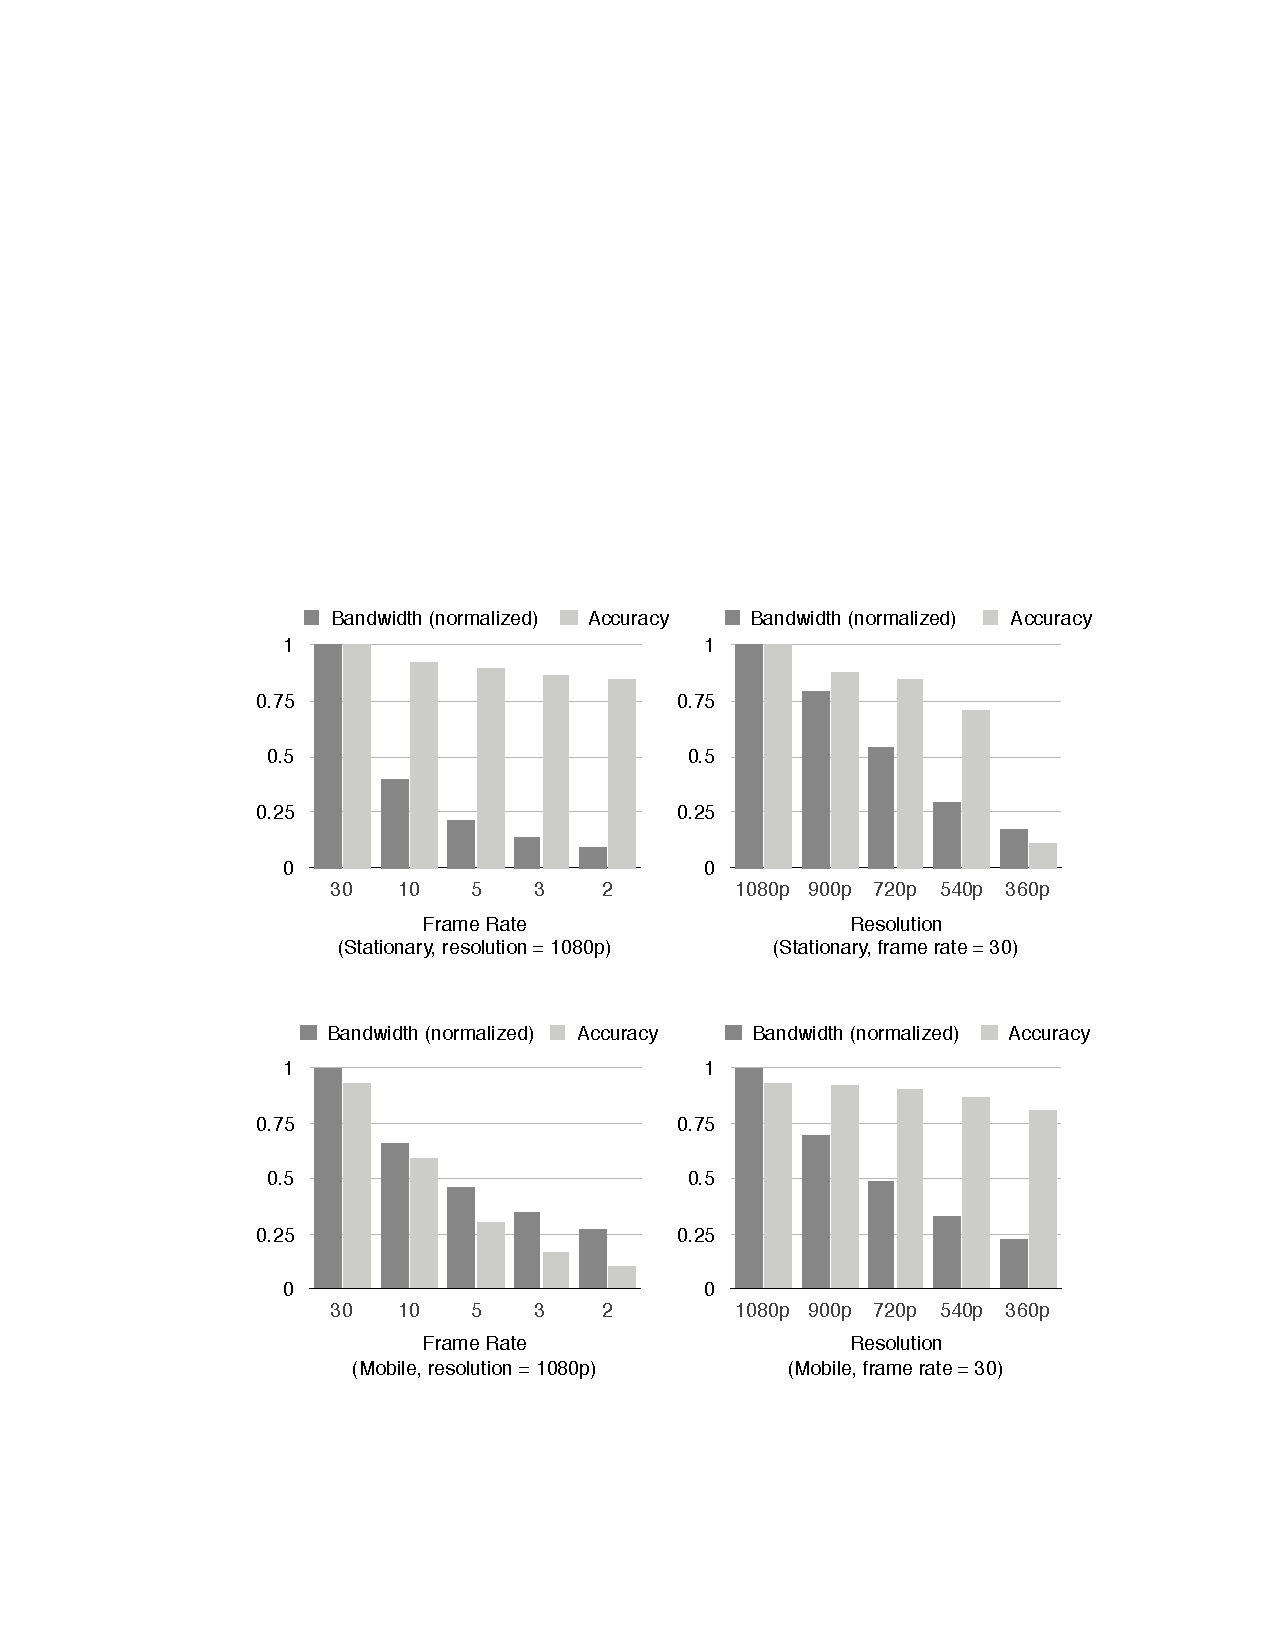
\includegraphics[width=\linewidth]{figures/motiv.pdf}
  \caption{Horizontally, how reducing the frame rate or resolution affects the
    bandwidth requirement and appliation accuracy. Vertically, how the same
    degradation have different impact for different data characteristics; the
    upper figures are for a stationary camera deployment while the lower figures
    are for mobile applications.}
  \label{fig:motiv}
\end{figure}

This motivates us to take a system-level approach that synthesizes different
adaptation strategies for different queries and contexts.

\section{Related Work}
\label{sec:related-work}

\paraf{Stream processing systems:} Streaming databases, such as
Borealis~\cite{abadi2005design},
TelegraphCQ~\cite{chandrasekaran2003telegraphcq}, are the early academic
explorations. They pioneered the usage of dataflow models with specialized
operators for stream processing. Recent research projects and open-source
systems, such as MillWheel~\cite{akidau2013millwheel},
Storm~\cite{toshniwal2014storm}, Heron~\cite{kulkarni2015twitter}, Spark
Streaming~\cite{zaharia2012discretized}, Apache Flink~\cite{carbone2015apache},
primary focus on fault-tolerant streaming in the context of a single
cluster. While this thesis has a large debt to the prior streaming work,
\sysname{} is designed for the wide-area and explicitly trades data fidelity for
data freshness; many other stream processing systems choose to throttle the
source when backpressure happens~\cite{kulkarni2015twitter}.

\para{WAN-aware:} There is a growing interest in building systems that optimizes
data transfers for the wide area, such as GDA~\cite{pu2015low},
Clarinet~\cite{viswanathan2016clarinet} and OWAN~\cite{jin2016optimizing}.  Most
of these works focus on one-time queries or operations (such as data
transfer). JetStream~\cite{rabkin2014aggregation} is the first that studies
streaming analytics in wide area and proposes to use structured storage (data
cubes) and explicit degradation policies. While JetStream has demonstrated
application responsiveness with hand-written degradation policy, these policies
are often developer heuristics that are not backed up by measurements. This
thesis extends the idea of degradation with an automatic policy synthesis.

\para{Approximate analytics:} The idea of degrading computation fidelity for
responsiveness has also been explored in other contexts, primarily SQL
queries. Online aggregation~\cite{hellerstein1997online},
BlinkDB~\cite{agarwal2013blinkdb} and GRASS~\cite{ananthanarayanan2014grass}
speed up queries with partial data based on a statistical model of SQL
operators. \sysname{} is different from these approximatte analytics as it
supports arbitrary data processing pipelines where no close-form solution exists
to evalute the impact of a particular degradation.

\para{Adaptive video streaming:} This is both an active research
topic~\cite{sun2016cs2p, yin2015control} with many trending industrial efforts.
Because they target at video delivery for web applications, many have chosen to
tune HTTP protocols for video adaptation, such as HLS~\cite{pantos2016http} by
Apple and DASH~\cite{michalos2012dynamic} as the new standard. The main
technique is to adjust the video resolution and encoding bitrate but they often
guarantee a smooth video with high frame rate (at least 25 FPS). This thesis
generalizes the adaptation to a wider range of streaming analytics and allows
more custom control over what parameters can be adjusted. \sysname{}
applications utilize existing techniques from adaptive video streaming (such as
H.264~\cite{richardson2011h} and VP9~\cite{grange2016vp9}) instead of
reinventing the wheel.

%%% Local Variables:
%%% mode: latex
%%% TeX-master: "../thesis"
%%% End:

% \chapter{Network Resource Adaptation}
\label{cha:netw-reso-adapt}

This chapter features AWStream.

\section{Introduction}

%% Background
Wide-area streaming analytics are becoming pervasive, especially with emerging
Internet of Things (IoT) applications. Large cities such as London and Beijing
have deployed millions of cameras for surveillance and traffic
control~\cite{skynet, london.surveillance}. Buildings are increasingly equipped
with a wide variety of sensors to improve energy efficiency and occupant
comfort~\cite{krioukov2012building}. Geo-distributed infrastructure, such as
content delivery networks (CDNs), analyze requests from machine logs across the
globe~\cite{mukerjee2015practical}. These applications all transport, distill,
and process streams of data across the wide area, in real time.

A key challenge that the above applications face is dealing with the scarce and
variable bandwidth in the wide area~\cite{hsieh17gaia, vulimiri2015global}.  As
many have observed, WAN bandwidth growth has been decelerating for many years
while traffic demands are growing at a staggering
rate~\cite{global2016telegeography, cisco2013zettabyte, cisco2016global}.  In
addition, scarcity in last-mile bandwidth remains a problem across
wireless~\cite{biswas2015large}, cellular~\cite{nikravesh2014mobile}, and even
broadband~\cite{grover2013peeking, sundaresan2014bismark} networks.  Finally, as
we elaborate on in \autoref{sec:motivation}, not only is WAN bandwidth scarce,
it is also relatively expensive, and highly variable.

For all of the above reasons, it is important that streaming applications be
\emph{adaptive}, incorporating the ability to optimally trade-off accuracy for
bandwidth consumption and hence a key system challenge is to design the
\emph{programming abstractions and tools} that simplify the development of such
adaptive applications.

In recent years, systems such as Storm~\cite{toshniwal2014storm}, Spark
Streaming~\cite{zaharia2013discretized}, and VideoStorm~\cite{zhang2017live},
have emerged in support of stream processing.  These systems enable efficient
processing of large streams of data, but are designed to work within a single
datacenter cluster (where network bandwidth is typically not the bottleneck) and
hence they do not focus on support for adapting to the vagaries of WAN
bandwidth.

Recent research on WAN-aware systems promote pushing computation to the network
edge~\cite{rabkin2014aggregation, satyanarayanan2009case}.  However, even with
edge computing, the need for adaptation remains because end-devices such as
cameras and mobile phones still suffer from limited bandwidth in the last-hop
infrastructure~\cite{abari2017enabling, zhang2015design}.  In addition, edge
computing is not a panacea as wide-area communication is often not entirely
avoidable: e.g., some analytical jobs require joining or aggregating data from
multiple geo-distributed sites~\cite{pu2015low, viswanathan2016clarinet}, while
in some cases processing benefits substantially from specialized computing
resources such as GPUs and TPUs~\cite{abadi2016tensorflow} in the cloud.

The core difficulty with adaptive streaming analytics is that, when bandwidth is
scarce, developers are faced with the decision of how to reconcile data fidelity
(i.e., not losing any data) with data freshness (i.e., sending data as quickly
as possible). A deterioration in either fidelity or freshness can impact
application accuracy but the exact impact varies depending on the
application.\footnote{E.g., an application tracking the current value of a
  variable might prioritize freshness while one that is computing an average
  might prioritize fidelity.} \autoref{fig:intro} illustrates this trade-off
with a few sample points in the design space.

\begin{figure}
  \centering
  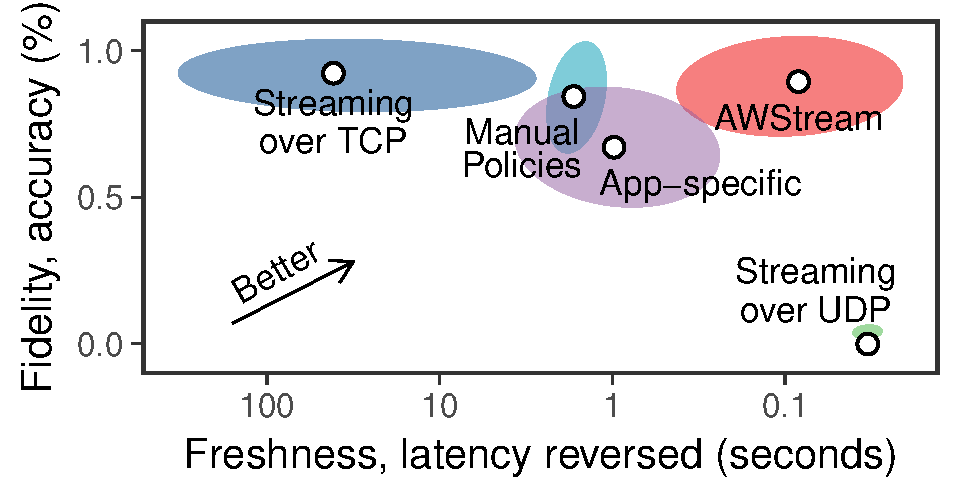
\includegraphics[width=0.8\columnwidth]{figures/figure1.pdf}
  \caption{The trade-off space between data freshness and fidelity when facing
    insufficient bandwidth (details in \autoref{sec:runtime-adaptation}).}
  \label{fig:intro}
  \vspace{-1em}
\end{figure}

Applications that simply use existing protocols without any attempt at
adaptation can result in extreme design points. E.g., streaming over TCP ensures
reliable delivery (hence high fidelity) but backlogged data delays the delivery
of data (hence freshness suffers).  On the other hand, streaming over UDP
minimizes latency by sending packets as fast as possible, but uncontrolled
packet loss can devastate data fidelity.

Manual policies, such as sampling, allow developers to trade data fidelity for
freshness~\cite{rabkin2014aggregation}. However, it's difficult to write
accurate policies without extensive domain expertise or considerable effort. In
practice, developers write manual policies based on heuristics rather than
quantitative measurements and, as we show in \autoref{sec:evaluation}, such
policies can lead to sub-optimal performance in terms of both freshness and
fidelity.

Furthermore, application-specific optimizations often do not generalize. A
fine-tuned adaptation algorithm for one application works poorly for a different
application, if performance metrics or data distributions change.  For example,
video streaming focuses on quality of experience
(QoE)~\cite{michalos2012dynamic, pantos2016http, yin2015control}. Because humans
favor smoothness over image quality, these systems maintain a high frame rate,
e.g.\,\(25~\text{FPS}\), and reduce the resolution under bandwidth limitation.
However, low resolution images can lead to poor accuracy for video analytics
that rely on the image details, e.g.\,face detection~\cite{viola2001rapid}.

In this paper, we present \sysname{}, a framework for building adaptive stream
processing applications that simultaneously simplifies development \emph{and}
improves application accuracy in the face of limited or varying wide-area
bandwidth.
% for the wide area that achieves low latency and high accuracy simultaneously
% with minimal developer effort.
\sysname{} achieves this through the combination of three novel contributions:

\begin{enumerate}[leftmargin=*]
\item \sysname{} introduces new programming abstractions by which a developer
  expresses \emph{what} degradation functions can be used by the framework.
  % {\bf Sylvia: Cut remainder of para? Too much detail for intro?}  More
  % specifically, \sysname{} augments existing stream processing operators with
  % a new \maybe{} operator. Its basic form takes a function that degrades the
  % input stream, and a list of values that serve as a knob to control the level
  % of degradation.  and . The knob specifies the degradation level that affects
  % data size and data fidelity.  We extend the basic form with a library of
  % specialized operators for common data types, such as
  % \texttt{maybe\_downsample} for images.  Our API is \textit{composable}
  % (multiple operators form a configuration that affects the adaptation
  % jointly), and \textit{extensible} (arbitrary functions and external
  % libraries can be embedded with our operators).
  Importantly, developers do not have to specify exactly when and how different
  degradation functions are to be used which is instead left to the \sysname{}
  framework.

\item Rather than rely on manual policies, \sysname{} automatically
  \emph{learns} a Pareto-optimal policy or strategy for when and how to invoke
  different degradation functions.  For this, we design a methodology that uses
  a combination of offline and online training to build an accurate model of the
  relationship between an application's accuracy and its bandwidth consumption
  under different combinations of degradation functions. Our solution exploits
  parallelism and sampling to efficiently explore the configuration space and
  learn an optimal strategy.

  % The key idea is to \textit{automatically} build an accurate and precise
  % \textit{performance model} instead of relying on manual policies or
  % application-specific optimizations.
  % We use an \textit{offline} process to bootstrap our system with
  % developer-supplied training data, and continuously refine the profile
  % \textit{online} to handle \textit{model drift}.  We exploit parallelism and
  % sampling-based techniques to efficiently explore the configuration space and
  % learn a adaptation strategy.

\item \sysname{}'s final contribution is the design and implementation of a
  runtime system that continually measures and adapts to network conditions.
  \sysname{} matches the streaming data rate to the measured available
  bandwidth, and achieves high accuracy by using the learned Pareto-optimal
  configurations.  Upon encountering network congestion, our adaptation
  algorithm increases the degradation level to reduce the data rate, such that
  no persistent queue builds up. To recover, it progressively decreases the
  degradation level after probing for more available bandwidth.

  % The runtime also provides additional options to control application
  % behaviors, such as limiting the maximum
  % allowed WAN bandwidth. For multiple applications, the profiles can be used
  % to allocate bandwidth among competing tasks for \textit{utility fairness}.
\end{enumerate}

We implement \sysname{} and use it to prototype three streaming applications:
augmented reality (AR), pedestrian detection (PD), and distributed Top-K
(TK). We use real-world data to profile these applications and evaluate their
runtime performance on a geo-distributed public cloud.  We show that
\sysname{}'s data-driven approach generates accurate profiles and that our
parallelism and sampling techniques can speed up profiling by up to 29$\times$
and 8.7$\times$\@ respectively.

We show that \sysname{} significantly outperforms non-adaptive applications:
e.g., achieving a 40--100$\times$ reduction in packet delivery times relative to
applications built over TCP, or an over 45--88\% improvement in data fidelity
(application accuracy) relative to applications built over UDP.  We also compare
\sysname{} to JetStream~\cite{rabkin2014aggregation}, a state-of-the-art system
for building adaptive streaming analytics that is based on manual policies: our
results show that besides the benefit of generating optimal policies
\textit{automatically}, \sysname{} achieves a 15-20$\times$ reduction in latency
and 1-5\% improvement in accuracy relative to JetStream. We show that these
gains come from the combination of \sysname{}'s ability to learn better policies
\emph{and} its well-designed runtime.  Hence, the ease of development that
\sysname{} provides comes with significantly \emph{improved} application
performance compared to typical manually crafted policies.

%%% Local Variables:
%%% mode: latex
%%% TeX-master: "../awstream"
%%% End:

%% LocalWords: VideoStorm analytics CDN CDNs geo IoT TCP UDP QoE runtime
%% LocalWords: GPUs TPUs downsample composable TK JetStream datacenter
\section{Motivation}
\label{sec:motivation}

In this section, we first examine the gap between high application demands and
limited WAN bandwidth. We then show that neither manual policies nor
application-specific optimizations solve the problem.

\subsection{Wide-area Streaming Applications}
\label{sec:wide-area-streaming}

We focus on wide-area streaming analytics, especially the emerging IoT
applications. We give two concrete examples.

\para{Video Surveillance.} We envisage a city-wide monitoring system that
aggregates camera feeds, from stationary ground cameras and moving aerial
vehicles, and analyzes video streams in real time for surveillance, anomaly
detection, or business intelligence~\cite{oh2011large}. Recent advances in
computer vision have dramatically increased the accuracy for automatic visual
scene analysis, such as pedestrian detection~\cite{dollar2012pedestrian},
vehicle tracking~\cite{coifman1998real}, and facial recognition to locate people
of interest~\cite{Lu:2015:SHF:2888116.2888245, parkhi2015deep}. While some
surveillance cameras use dedicated links, an increasing number of surveillance
systems, such as Dropcam~\cite{dropcam} and Vigil~\cite{zhang2015design}, use
the public Internet and wireless links to reduce the cost of deployment and
management.

% \para{High-frequency IoT Sensors:} Although environmental sensors used to be
% slow and not data-intensive~\cite{atzori2010internet}, increasingly,
% high-frequency, high-precision sensors are deployed. For example, uPMUs
% monitor the electrical grid with a network of 1000 devices; each produces 12
% streams of 120 Hz high-precision values accurate to 100 ns. This amounts to
% 1.4 million points per second~\cite{andersen2016btrdb}.

\para{Infrastructure Monitoring.} Large organizations today are managing tens of
datacenters and edge clusters worldwide~\cite{calder2013mapping}. This
geo-distributed infrastructure continuously produces large volumes of data such
as data access logs, server monitoring logs, and performance
counters~\cite{alspaugh2014analyzing, pu2015low, vulimiri2015global}. While most
log analysis today runs in a batch mode on a daily basis, there is a trend
towards analyzing logs in real time for rapid
optimization~\cite{rabkin2014aggregation}. For example, CDNs can improve the
overall efficiency by optimizing data placement if the access logs can be
processed in real time. In Industrial IoT, large-scale real-time sensor
monitoring is becoming pervasive to detect anomalies, direct controls, and
predict maintenance ~\cite{balani2016enterprise, ge}.

%% ~\cite{xu2009detecting} We generated the HDFS logs by setting up a Hadoop
%% cluster on 203 EC2 nodes and running sample Hadoop map-reduce jobs for 48
%% hours, generating and processing over 200 TB of random data. We collected
%% over 24 million lines of logs from HDFS.

% We consider the practical issues with deploying these applications in the
% wide-area. Our stand is that these applications face a bigger network
% challenge.  Data generated from the edge often fail to be delivered to the
% processing site because of the scarce and variable bandwidth capacity in the
% wide-area. Once they arrive, existing stream processing systems can easily
% manage a large cluster and perform data analytics at real-time.

\subsection{Wide-area Bandwidth Characteristics}
\label{sec:wide-area-bandwidth}

WAN bandwidth is insufficient and costly, as shown by other
systems~\cite{hsieh17gaia, pu2015low, vulimiri2015wananlytics,
  vulimiri2015global}. Using Amazon EC2 as a case study, the WAN bandwidth
capacity is 15x smaller than their LAN bandwidth on average, and up to 60x
smaller in the worst case~\cite{hsieh17gaia}. In terms of pricing, the average
WAN bandwidth cost is up to 38x of the cost of renting two
machines~\cite{amazon2017pricing, hsieh17gaia}.

In addition to the scarcity and cost, the large variability of WAN bandwidth
also affects streaming workloads. We conducted a day-long measurement with
iPerf~\cite{iperf3} to study the pair-wise bandwidth between four Amazon EC2
sites (N. California, N. Virginia, Tokyo, Ireland).  The results show large
variance in almost all pairs---\autoref{fig:bw} is one such pair. There are
occasions when the available bandwidth is below 25\% of the maximum bandwidth.

\begin{figure}
  \centering
  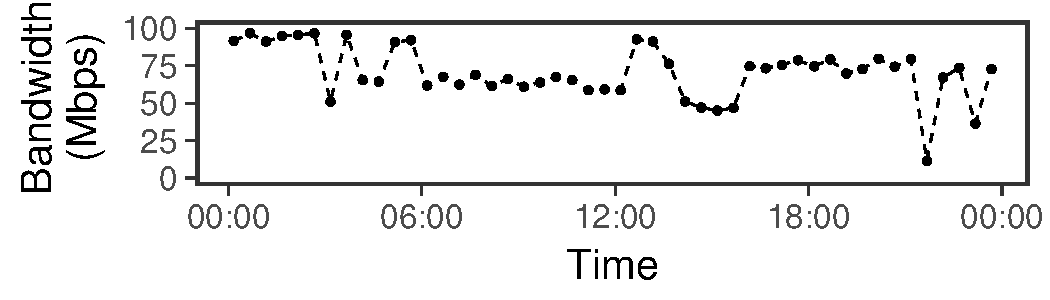
\includegraphics[width=0.9\linewidth]{figures/aws-variation.pdf}
  \caption{Bandwidth variations throughout the day between Amazon EC2 sites
    (from Ireland to California).}
  \label{fig:bw}
  \vspace{-1em}
\end{figure}

The back-haul links between EC2 sites are better---if not at least
representative---in comparison to general WAN links. Similar scarcity and
variations exist in wireless networks~\cite{biswas2015large}, broadband access
networks~\cite{grover2013peeking, sundaresan2014bismark} and cellular
networks~\cite{nikravesh2014mobile}.

\subsection{Motivation for \sysname{}}
\label{subsec:motivation}

\begin{figure*}
  \centering
  \includegraphics[width=0.85\linewidth]{figures/motiv-app-specific.pdf}
  \caption{The measured bandwidth and application accuracy for two video
    analytics applications. (1) Manual policies lack precision without
    measurements and need to handle multiple dimensions (as in a-d). (2)
    Application-specific optimizations do not generalize: degrading frame rates
    works well for stationary camera (a), but not for mobile camera (c). (e-h)
    shows example frames.}
  \label{fig:app-specific}
\end{figure*}

To address bandwidth limits, existing solutions use manual policies or
application-specific solutions. We discuss their drawbacks to motivate
\sysname{} (design in \autoref{sec:system}).

\para{Manual polices are sub-optimal.} JetStream~\cite{rabkin2014aggregation} is
the first to use degradation to address bandwidth limits in wide area. While
effective in comparison to non-adaptive systems, JetStream requires developers
to write manual policies, e.g.~\textit{``if bandwidth is insufficient, switch to
  sending images at 75\% fidelity, then 50\% if there still isn't enough
  bandwidth. Beyond that point, reduce the frame rate, but keep the image
  fidelity.''}\footnote{Excerpt from JetStream \S
  4.3~\cite{rabkin2014aggregation}.} We discuss the problems with manual
policies below and present quantitative evaluations in
\autoref{sec:runtime-adaptation}.

First, this policy is not accurate.  Developers write such rules based on
heuristics and do not back them up with measurements. Images with 75\% fidelity
do not necessarily lead to 75\% application accuracy. In terms of bandwidth,
naively one would think that reducing the frame rate by half will also half the
data rate. But if video encoding such as H.264~\cite{richardson2011h} is used, a
reduction in frame rate increases the inter-frame difference and creates
P-frames with larger sizes. \hyperref[fig:app-specific]{Fig.~3c} shows that when
reducing the frame rate to 33\% (from \(30~\text{FPS}\) to \(10~\text{FPS}\)),
the bandwidth use can still be more than 50\%.

Second, it is not scalable to specify rules one by one. A fine-grain control
requires many rules in the policy. Besides, applications can degrade in multiple
dimensions and each dimension has different impacts (compare
\hyperref[fig:app-specific]{Fig.~3a} with \hyperref[fig:app-specific]{Fig.~3b}).
Specifying rules in detail and across dimensions manually is a tedious and
error-prone process.

Lastly, this abstraction is too low-level. It forces developers to study and
measure the impact of individual operations, prohibiting its wide adoption in
practice.

\para{Application-specific optimizations do not generalize.} Because each
application has different performance metrics and relies on different features,
a fine-tuned policy for one application will often work poorly for another. For
example, DASH~\cite{sodagar2011mpeg} optimizes QoE for video streaming; it keeps
a high frame rate and reduces resolutions for adaptation. Its policy that lowers
the resolution works poorly for video analytics that relies on image
details~\cite{lowe2004distinctive, viola2001rapid}. In
\hyperref[fig:app-specific]{Fig.~3b}, we show that pedestrian detection accuracy
drops fast when reducing resolutions as pedestrian are small in the scenes.

Similar applications face different data distributions, as shown in
\autoref{fig:app-specific} between stationary cameras detecting pedestrians (up)
and mobile cameras recognizing objects (bottom). For stationary cameras, when we
consider the slow walking speed of pedestrians, a high frame rate is not
necessary. But high-resolution images are crucial because these surveillance
cameras are far away from the targets. In the mobile camera case, because the
camera moves, reducing the frame rate introduces significant errors.

%%% Local Variables:
%%% mode: latex
%%% TeX-master: "../awstream"
%%% End:

%% LocalWords: Dropcam IoT DCs geo CDNs iPerf JetStream scalable
%% LocalWords: bw runtime QoE analytics datacenters

\section{\sysname{} Design}
\label{sec:system}

To address the issues with manual policies or application-specific
optimizations, \sysname{} structures adaptation as a set of approximate,
modular, and extensible specifications (\autoref{sec:structure-adapt}). The
well-defined structure allows us to build a generic profiling tool that learns
an accurate relationship---we call it the profile---between bandwidth
consumption and application accuracy (\autoref{sec:automatic-profiling}). The
profile then guides the runtime to react with precision: achieving low latency
and high accuracy when facing insufficient bandwidth
(\autoref{sec:runtime}). \autoref{fig:overview} shows the high-level overview of
\sysname{}.

\begin{figure}
  \centering
  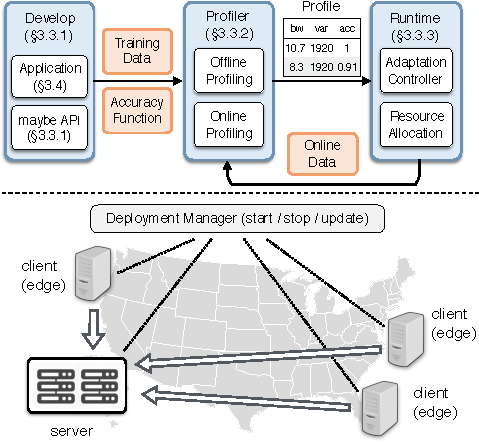
\includegraphics[width=0.9\linewidth]{figures/system.pdf}
  \caption{\sysname{}'s phases: development, profiling, and runtime. \sysname{}
    also manages wide-area deployment.}
  \label{fig:overview}
\end{figure}

\subsection{API for Structured Adaptation}
\label{sec:structure-adapt}

%% Introduce graphs of operators model
Most stream processing systems construct applications as a directed graph of
operators~\cite{toshniwal2014storm, zaharia2013discretized}. Each operator
transforms input streams into new streams. \sysname{} borrows the same
computation model.  \autoref{tab:operators} lists some example operators, such
as \texttt{map} and \texttt{skip}.

To integrate adaptation as a first-class abstraction, \sysname{} introduces
\maybe{} operators that degrade data quality, yielding potential bandwidth
savings.  Our API design has three considerations. $(i)$~To free developers from
specifying exact rules, the API should allow specifications with
options. $(ii)$~To allow combining multiple dimensions, the API should be
modular. $(iii)$~To support flexible integration with arbitrary degradation
functions, the API should take user-defined functions. Therefore, our API is,

\vspace{-2pt}
\begin{lstlisting}
        maybe(knobs: Vec<T>, f: (T, I) => I)
\end{lstlisting}

We illustrate the use of the \texttt{maybe} operator with an example that
quantizes a stream of integers in Rust:

\begin{table*}
  \small
  \centering
  \begin{tabular}{ c r l }
    \toprule
    \multirow{4}{*}{Normal Operators}
    & \textit{map} (f: I $\Rightarrow$ O) & Stream<I> $\Rightarrow$ Stream<O> \\
    & \textit{skip} (i: Integer) & Stream<I> $\Rightarrow$
                                   Stream<I> \\
    & \textit{sliding\_window} (count: Integer, f: Vec<I> $\Rightarrow$ O) & Stream<I> $\Rightarrow$
                                                                            Stream<O> \\
    % & \textit{tumbling\_window} (count: Integer, f: Vec<I> $\Rightarrow$ O) & Stream<I> $\Rightarrow$
    %                                                                          Stream<O> \\
    % & \textit{timed\_window} (time: Duration, f: Vec<I> $\Rightarrow$ O) & Stream<I> $\Rightarrow$
    %                                                                      Stream<O> \\
    & ... & ... \\
    \midrule
    \multirow{5}{*}{Degradation Operators}
    & \textit{maybe} (knobs: Vec<T>, f:  (T, I) $\Rightarrow$ I) & Stream<I> $\Rightarrow$
                                                                 Stream<I> \\
    & \textit{maybe\_skip} (knobs: Vec<Integer>) & Stream<I> $\Rightarrow$ Stream<I> \\
    & \textit{maybe\_head} (knobs: Vec<Integer>) & Stream<Vec<I>{}> $\Rightarrow$
                                                   Stream<Vec<I>{}> \\
    & \textit{maybe\_downsample} (knobs: Vec<(Integer, Integer)>) & Stream<Image> $\Rightarrow$ Stream<Image> \\
    & ... & ... \\
    \bottomrule
  \end{tabular}
  \vspace{0.2em}
  \caption{Stream processing operators in \sysname{}. \texttt{Vec<T>} represents
    a list of elements with type \texttt{T}.}
  \label{tab:operators}
  \vspace{-1em}
\end{table*}

\vspace{-2pt}
\begin{lstlisting}
let quantized_stream = vec![1, 2, 3, 4].into_stream()
    .maybe(vec![2, 4], |k, val| val.wrapping_div(k))
    .collect();
\end{lstlisting}

The snippet creates a stream of integers, chains a degradation operation, and
collects the execution result. In this example, the knob is [2, 4] and the
degradation function performs a wrapping (modular) division where the divisor is
the chosen knob. The knob value modifies the quantization level, affecting the
output: [1, 2, 3, 4] (no degradation), [0, 1, 1, 2] (k=2), or [0, 0, 0, 1]
(k=4). If the stream is then encoded---e.g. run-length encoding as in
JPEG~\cite{wallace1992jpeg}---for transmission, the data size will depend on the
level of degradation.

Based on the \texttt{maybe} primitive, one can implement additional degradation
operators for common data types. For instance, \texttt{maybe\_head} will
optionally take the top values of a list; \texttt{maybe\_downsample} can resize
the image to a configured resolution. \sysname{} provides a number of such
operations as a library to simplify application development
(\autoref{tab:operators}).

With our API, the example mentioned in \autoref{subsec:motivation} can now be
implemented as follows:

\vspace{-4pt}
\begin{lstlisting}
let app = Camera::new((1920, 1080), 30)
    .maybe_downsample(vec![(1600, 900), (1280, 720)])
    .maybe_skip(vec![2, 5])
    .map(|frame| frame.show())
    .compose();
\end{lstlisting}

This snippet first instantiates a \texttt{Camera} source, which produces
\texttt{Stream<Image>} with 1920x1080 resolution and 30 FPS\@. Two degradation
operations follow the source: one that downsamples the image to 1600x900 or
1280x720 resolution, and the other that skips every 2 or 5 frames, resulting in
30/(2+1)=10 FPS or 30/(5+1)= 6 FPS\@. This example then displays degraded
images. In practice, operators for further processing, such as encoding and
transmission, can be chained.

%%% Local Variables:
%%% mode: latex
%%% TeX-master: "../awstream"
%%% End:

%% LocalWords: UDFs Vec quantization quantized quantizes
%% LocalWords: downsample downsamples subsec resize

\subsection{Automatic Profiling}
\label{sec:automatic-profiling}

After developers use \maybe{} operators to specify potential degradation
operations, \sysname{} automatically builds an accurate profile. The profile
captures the relationship between \textit{application accuracy} and
\textit{bandwidth consumption} under different combinations of data degradation
operations. We describe the formalism, followed by techniques that efficiently
perform offline and online profiling.

\para{Profiling formalism.} Suppose a stream processing application has $n$
\maybe{} operators. Each operator introduces a knob $k_i$. The combination of
all knobs forms a \textit{configuration} $c = [k_{1}, k_{2}, ... k_{n}]$. The
set of all possible configurations $\mathbb{C}$ is the space that the profiling
explores. For each configuration $c$, there are two mappings that are of
particular interest: a mapping from $c$ to its bandwidth consumption $B(c)$ and
its accuracy measure $A(c)$. \autoref{tab:notations} summarizes these symbols.

The profiling looks for Pareto-optimal configurations; that is, for any
configuration $c$ in the Pareto-optimal set $\mathbb{P}$, there is no
alternative configuration $c'$ that requires less bandwidth and offers a higher
accuracy. Formally, $\mathbb{P}$ is defined as follows:

{\small \vspace{-1em}
  \begin{equation}
  \mathbb{P} = \{ c \in \mathbb{C} : \{ c' \in \mathbb{C}: B(c') < B(c),
  A(c') > A(c) \} = \varnothing\}
  \label{eq:pareto}
\end{equation}
}%

\begin{table}
  \footnotesize
  \centering
  \begin{tabular}{r l}
    \toprule
    \textbf{Symbol} & \textbf{Description} \\
    \midrule
    $n$ & number of degradation operations \\
    $k_i$ & the \textit{i}-th degradation knob \\
    $c = [k_{1}, k_{2}, ... k_{n}]$ & one specific configuration \\
    $\mathbb{C}$ & the set of all configurations \\
    \midrule
    $B(c)$ & bandwidth requirement for $c$ \\
    $A(c)$ & accuracy measure for $c$ \\
    $\mathbb{P}$ & Pareto-optimal set \\
    \midrule
    $c_i$, $c_{i+1}$, $c_{\max}$ & current/next/maximal configuration at runtime \\
    $R$ & network delivery rate (estimated bandwidth) \\
    $\text{Q}_\text{E}$, $\text{Q}_\text{C}$ & messages when \texttt{Queue} is empty or congested \\
    $\text{R}_\text{C}$ & message when \texttt{Receiver} detects congestion \\
    $\text{AC}_\text{Probe}$ & message when \texttt{AC} requests probing \\
    $\text{S}_\text{ProbeDone}$ & message when \texttt{Socket} finishes probing \\
    \bottomrule
  \end{tabular}
  \vspace{0.3em}
  \caption{Notations used in this paper.}
  \label{tab:notations}
  \vspace{-3em}
\end{table}

Because \sysname{} allows arbitrary functions as the degradation functions, it
does not assume a closed-form relationship for $B(c)$ and $A(c)$. Instead,
\sysname{} takes a data-driven approach: profiling applications with
developer-supplied training data.  We measure $B(c)$ at the point of
transmission. The accuracy $A(c)$ is measured either against the groundtruth, or
the reference results when all degradation operations are off.  We show examples
of knobs, configurations, and accuracy functions when we present applications in
\autoref{sec:implementation}.

\para{Offline Profiling.} We first use an offline process to build a bootstrap
profile (or default profile).  \sysname{} makes no assumptions on the
performance models, and thus evaluates all possible configurations.  While all
knobs form a combinatorial space, the offline profiling is only a one-time
process.  We exploit parallelism to reduce the profiling time.  Without any
\textit{a priori} knowledge, all configurations are assigned randomly to
available machines.

% \para{Offline Profiling.} We first use an offline process to build a bootstrap
% profile (or default profile).  Because \sysname{} supports arbitrary
% degradation operations, we need to evaluate all combinations of the
% configurations offline profiling is a one-time process, \sysname{} currently
% performs an exhaustive evaluation of all configurations in $\mathbb{C}$
% despite all knobs form a combinatorial space. Future work could explore
% statistical methods to build performance models with a smaller number of
% training samples~\cite{venkataraman2016ernest, alipourfard2017cherrypick}.
% \sysname{} exploits parallelism when profiling all configurations.  Without
% any \textit{a priori} knowledge, all configurations are assigned randomly to
% all available machines.

\para{Online Profiling:} \sysname{} supports online profiling to continuously
refine the profile. The refinement handles \textit{model drift}, a problem when
the learned profile fails to predict the performance accurately. There are two
challenges with online profiling.  $(i)$~There are no ground-truth labels or
reference data to compute accuracy. Because labeling data is prohibitively labor
intensive and time consuming~\cite{russell2008labelme}, \sysname{} currently
uses raw data (data without degradation) as the reference. At runtime, if the
application streams raw data, it is used for online profiling. Otherwise, we
allocate additional bandwidth to transmit raw data, but only do so when there is
spare capacity. $(ii)$~Exhaustive profiling is expensive. If the profiling takes
too much time, the newly-learned profile may already be stale. \sysname{} uses a
combination of parallelization and sampling to speed up profiling, as below:

\begin{itemize}[leftmargin=*, topsep=3pt]

\item Parallelization with degradation-aware scheduling. Evaluating each
  configuration takes a different amount of time. Typically, an increase in the
  level of degradation leads to a decrease in computation; for example, a
  smaller FPS means fewer images to process. Therefore, we collect processing
  times for each configuration from offline profiling and schedule online
  profiling with longest first schedule (LFS)~\cite{karger2010scheduling} during
  parallelization.

\item Sampling-based profiling. Online profiling can speed up when we sample
  data or configurations. Sampling data reduces the amount of data to process,
  but at a cost of generating a less accurate profile. When sampling
  configuration, we can evaluate a subset of the Pareto-optimal configurations
  and compare their performances with an existing profile. A substantial
  difference, such as more than \SI{1}{Mbps} of bandwidth estimation, triggers a
  full profiling over all configurations to update the current profile.

\end{itemize}

%%% Local Variables:
%%% mode: latex
%%% TeX-master: "../awstream"
%%% End:

%% LocalWords: ProbeDone th combinatorial runtime parallelization priori
%% LocalWords: LFS mbps groundtruth
\subsection{Runtime Adaptation}
\label{sec:runtime}

At runtime, \sysname{} matches data rate to available bandwidth to minimize
latency and uses Pareto-optimal configurations to maximize accuracy. This
section focuses on the details of our runtime design. We defer the evaluation
and comparisons with existing systems (e.g.\,JetStream) to
\autoref{sec:runtime-adaptation}.

\begin{figure}
  \centering
  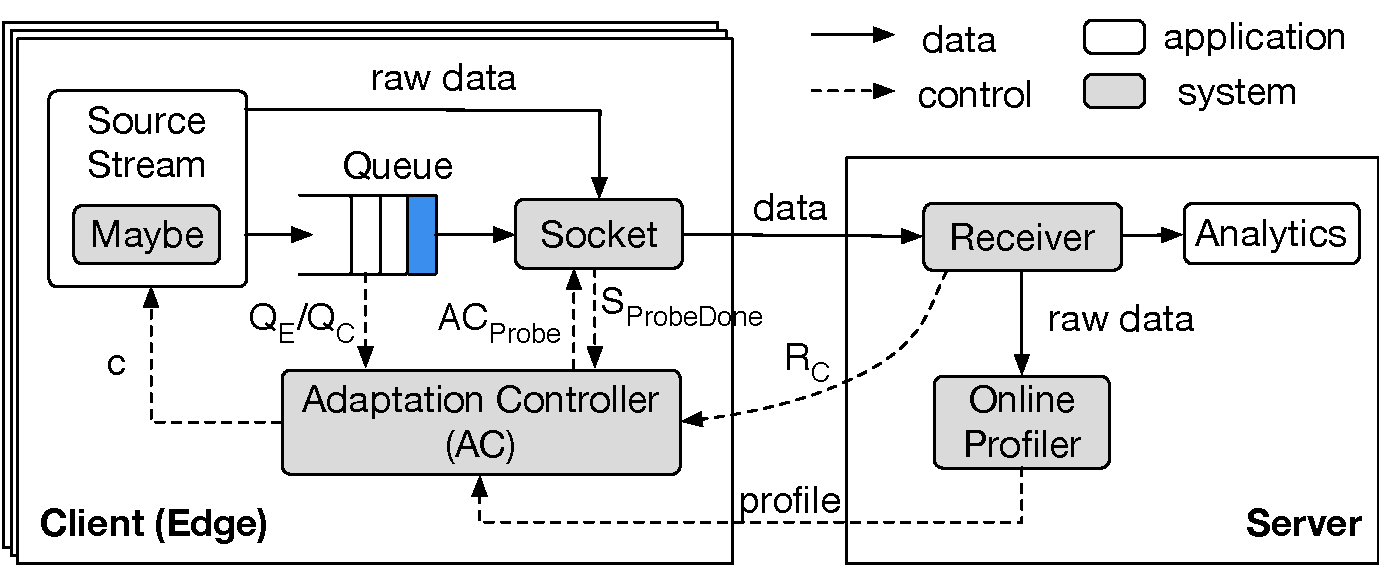
\includegraphics[width=\linewidth]{figures/runtime-adaptation.pdf}
  \caption{Runtime adaptation system architecture.}
  \label{fig:runtime}
\end{figure}

\autoref{fig:runtime} shows our runtime system architecture. \sysname{}
applications' source contains a \texttt{Maybe} module derived from all \maybe{}
operators. This module allows the controller to update the level of
degradation. Data generated by the source is then enqueued to \texttt{Queue} and
subsequently dequeued by \texttt{Socket}, which sends data over the network
using TCP. When the data generation rate exceeds \texttt{Socket}'s departure
rate, the queue grows. In this case, the adaptation controller (AC) queries the
estimated bandwidth from \texttt{Socket} and regulates the source stream by
updating the configuration. After the data is sent through the network,
\texttt{Receiver} delivers data to the application analytics. \texttt{Receiver}
also performs congestion detection and extracts raw data, if it is present.  It
tracks the minimal latency (similar to how BBR tracks
\texttt{RTprop}~\cite{cardwell2017bbr}) and reports sudden application-level
latency spikes to clients as congestion signals (\rc{}). If a new profile is
learned by the online profiler, it is fed back to AC for subsequent adaptation.

\autoref{fig:cc-sm} shows the adaptation algorithm with a state machine model
and \autoref{fig:cc-ex} shows the state transitions with an example. We first
describe all symbols. AC loads the profile and sorts all configurations with an
ascending order of bandwidth demand, resulting in a list
$[c_1, \dots, c_{\max}]$.  These configurations follow a total order:
$c_i < c_j$ if $B(c_i) < B(c_j)$.  We denote the current configuration as $c_i$
and the next $c_{i+1}$.  AC receives messages from other modules: \qe{} when
\texttt{Queue} is empty; $\text{Q}_\text{C}$ when queued items exceed a
threshold; and \rc{} when \texttt{Receiver} detects congestion. AC can query
\texttt{Socket} for delivery rate $R$ (arrow not shown) or request it to probe
($\text{AC}_{\text{Probe}}$) for a target bandwidth, often $B(c_{i+1})$. If
there is no congestion during the probing and $R > B(c_{i+1})$, \texttt{Socket}
sends back \spd{}. Below, we describe each state and transitions.

\begin{figure}
  \begin{subfigure}[t]{\columnwidth}
    \centering
    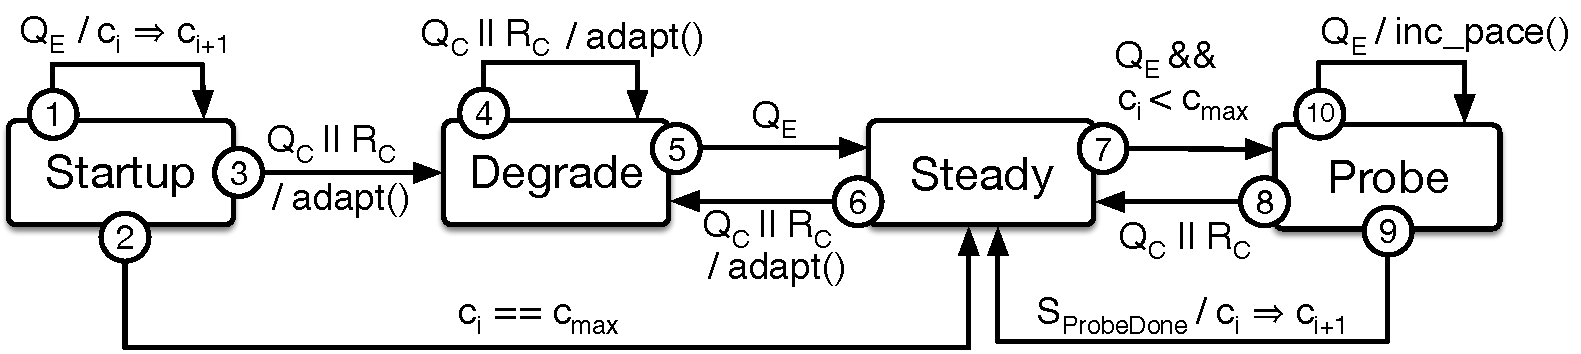
\includegraphics[width=\columnwidth]{figures/cc.pdf}
    \caption{Rate adaptation as a state machine.}
    \label{fig:cc-sm}
  \end{subfigure}
  \vspace{0.5em}
  \\
  \centering
  \begin{subfigure}[t]{\columnwidth}
    \centering
    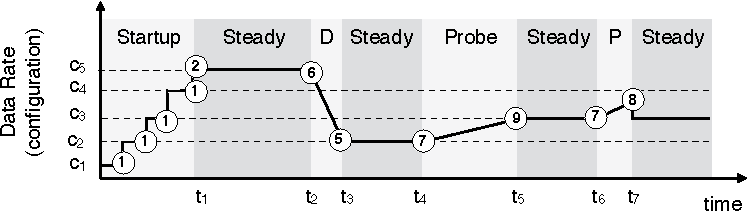
\includegraphics[width=0.9\columnwidth]{figures/cc2.pdf}
    \caption{An example illustrating the adaptation algorithm.}
    \label{fig:cc-ex}
  \end{subfigure}
  \caption{Runtime adaptation algorithm.}
  \label{fig:cc}
\end{figure}

\begin{itemize}[leftmargin=*, topsep=3pt, itemsep=0pt]

\item \textbf{Startup: rapid growth.} \sysname{} starts with $c_1$ and grows the
  rate ($c_i \Rightarrow c_{i+1}$) upon each \qe{}. The growth stops at
  $c_{\max}$ (to \texttt{Steady}) or if it receives \qc{}/\rc{} (to
  \texttt{Degrade}).

\item \textbf{Degrade: reacting to congestion.} Congestion is detected in two
  ways: (1) when \texttt{Queue} grows and exceeds a threshold, AC receives
  \qc{}; (2) when \texttt{Receiver} detects latency spikes, AC receives
  \rc{}. During congestion, AC runs the \texttt{adapt()} procedure by updating
  \texttt{Maybe} with the maximum-allowed $c$ that satisfies $B(c) < \alpha R$,
  where $\alpha \in (0, 1)$ and $R$ is \texttt{Socket}'s current delivery
  rate. A smaller $\alpha$ allows a quicker draining of the queue. After the
  congestion is resolved (\qe{} received), \sysname{} changes to
  \texttt{Steady}.

\item \textbf{Steady: low latency delivery.} \sysname{} achieves low latency by
  spending most of the time in \texttt{Steady}. It changes to \texttt{Degrade}
  when congestion occurs. If $c < c_{\max}$ and it receives \qe{}, AC starts
  \texttt{Probe} to check for more available bandwidth.

\item \textbf{Probe: more bandwidth for a higher accuracy.} Advancing $c_i$
  directly may cause congestion if $B(c_{i+1}) \gg B(c_i)$. To allow a smooth
  increase, AC requests \texttt{Socket} to probe by sending additional traffic
  controlled by \texttt{probe\_gain} (in \texttt{inc\_pace()}, similar to
  BBR~\cite{cardwell2017bbr}). Raw data is used for probing if available,
  otherwise we inject dummy traffic. \sysname{} stops probing under two
  conditions: (1) upon \spd{}, it advances $c_i$; (2) upon \qc{} or \rc{}, it
  returns to \texttt{Steady}. The explicit \texttt{Probe} phase stabilizes
  feedback loop and prevents oscillation.

\end{itemize}


\subsection{Resource Allocation \& Fairness}

In addition to rate adaptation, the profile is also useful for controlling a
single application's bandwidth usage or allocating resources among competing
tasks.

For individual applications, developers can pin-point a configuration for a
given bandwidth or accuracy goal. They can also specify a criterion to limit
effective configurations. For example, \sysname{} can enforce an upper bound on
the bandwidth consumption (e.g.,~do not exceed \SI{1}{Mbps}) or a lower bound on
application accuracy (e.g.,~do not fall below 75\%).

For multiple applications, their profiles allow novel bandwidth allocation
schemes such as utility fairness. Different from resource fairness with which
applications get an equal share of bandwidth, utility fairness aims to maximize
the \textit{minimal} application accuracy. With the profiles, bandwidth
allocation is equivalent to finding proper configuration $c^t$ for application
$t$. We formulate utility fairness as follows:

%% Pick one based on the space

\vspace{-0.5em}
\begin{equation}
  \vspace{-0.5em}
  \label{eq:multitask}
 \underset{c^t}{\max} \; \min({A^t(c^t)})
 \;
 \text{s.t.}
 \;
 \sum_t{B^t(c^t)} < R
\end{equation}

% \begin{equation}
%  \label{eq:multitask}
%  \begin{aligned}
%     & \underset{c^t}{\text{maximize}} & & \min({A^t(c^t)}) & & \\
%     & \text{subject to} & & \sum_t{B^t(c^t)} < R & & \\
%  \end{aligned}
% \end{equation}

Solving this optimization is computationally hard. \sysname{} uses heuristics
similar to VideoStorm~\cite{zhang2017live}: it starts with $c^t_1$ and improves
the application $t$ with the worst accuracy; this process iterates until all
bandwidth is allocated.

%%% Local Variables:
%%% mode: latex
%%% TeX-master: "../awstream"
%%% End:

%% LocalWords: runtime analytics enqueued dequeued TCP JetStream
%% LocalWords: RTprop BBR profiler sm VideoStorm

%%% Local Variables:
%%% mode: latex
%%% TeX-master: "../../thesis"
%%% End:

\section{Implementation}
\label{sec:implementation}

While our proposed API is general and not language specific, we have implemented
\sysname{} prototype in Rust (\textasciitilde 4000 lines of code). \sysname{} is
open source on GitHub.\footnote{URL elided for anonymity.}  Applications use
\sysname{} as a library and configure the execution mode---profiling, runtime as
client, or runtime as server---with command line arguments.

% \begin{figure}
%   \centering
%   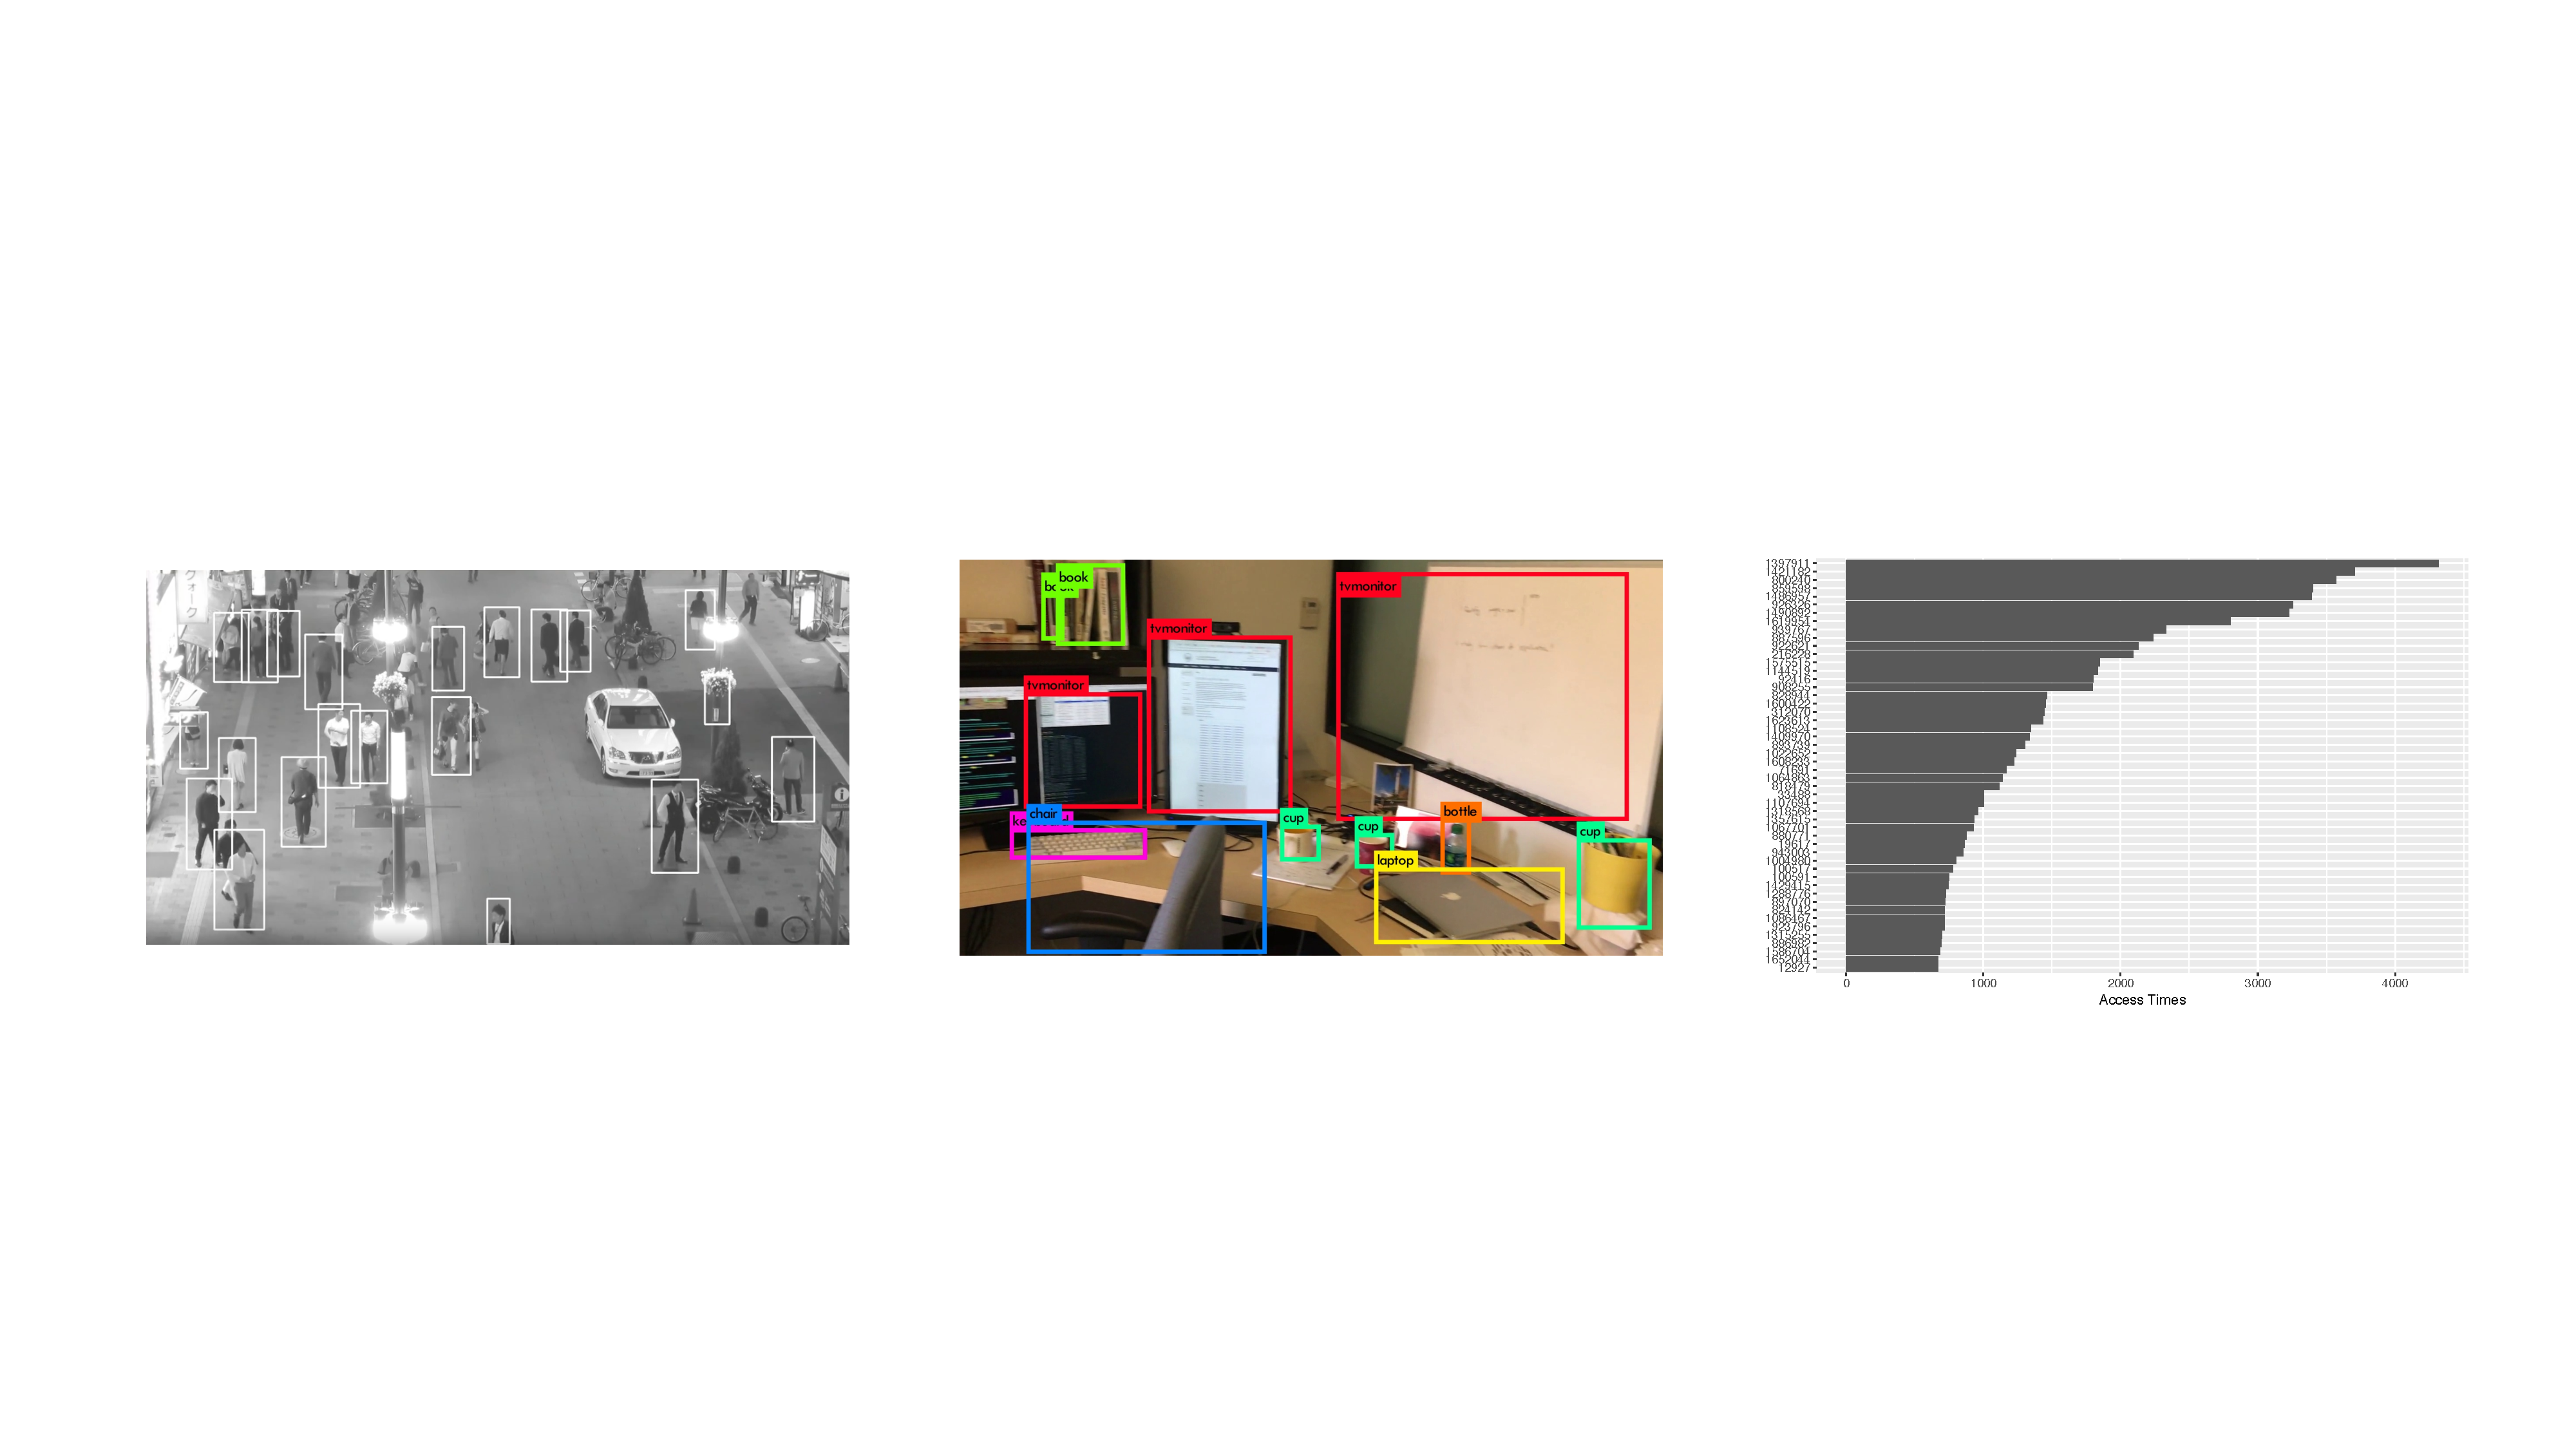
\includegraphics[width=\columnwidth]{figures/apps.pdf}
%   \caption{Three \sysname{} applications: augmented reality, pedestrian
%     detection, and distributed Top-K.}
%   \label{fig:three-apps}
% \end{figure}

\begin{table}
  \footnotesize
  \centering
  \begin{tabular}{c c c c}
    \toprule
    Application & Knobs & Accuracy & Dataset \\
    \midrule
    \specialcell{Augmented\\Reality}
                & \specialcell{resolution \\ frame rate \\ quantization }
                & F1 score~\cite{Rijsbergen:1979:IR:539927}
                & \specialcell{iPhone video clips\\training: office (24
    s)\\testing: home (246 s)} \\
    \midrule
    \specialcell{Pedestrian\\Detection}
                & \specialcell{resolution \\ frame rate \\ quantization }
                & F1 score
                & \specialcell{MOT16~\cite{milan2016mot16}\\training: MOT16-04\\testing: MOT16-03} \\
    \midrule
    \specialcell{Log Analysis\\(Top-K, K=50)}
                & \specialcell{head (N) \\ threshold (T) }
                & \specialcell{Kendall's $\tau$~\cite{abdi2007kendall}}
                & \specialcell{\href{https://www.sec.gov}{SEC.gov} logs~\cite{edgarlog} \\ training: 4 days \\
    testing: 16 days} \\
    \bottomrule
  \end{tabular}
  \vspace{0.5em}
  \caption{Application details.}
  \label{tab:apps}
  \vspace{-1em}
\end{table}

Using \sysname{}, we have built three applications: augmented reality (AR) that
recognizes nearby objects on mobile phones, pedestrian detection (PD) for
surveillance cameras, and a distributed log analysis to extract the Top-K mostly
accessed files (TK). \autoref{tab:apps} summarizes the application-specific
parts: knobs, accuracy functions, and datasets.

\para{Augmented Reality.} We target at augmented reality applications running on
mobile phones that recognize nearby objects by offloading the heavy computation
elsewhere, e.g.\,the cloud.

Our implementation uses OpenCV~\cite{opencvlibrary} for image-related operations
and YOLO~\cite{darknet13, redmon2016yolo9000}, a GPU-enabled pre-trained neural
network, for object recognition. Videos are encoded with
H.264~\cite{richardson2011h}. Our implementation uses GStreamer~\cite{gstreamer}
with \texttt{x264enc} plugin (\texttt{zerolatency} and constant quality). The
quantization factor affecting encoding quality becomes a knob in addition to
image resolutions and frame rates.

Object recognition returns a list of bounding boxes with the object type. Each
bounding box is a rectangle with normalized coordinates on the image. We compare
the detection against the reference result from raw data, and declare it success
if the intersection over union (IOU) is greater than
50\%~\cite{everingham2010pascal} and the object type matches. We use F1
score~\cite{Rijsbergen:1979:IR:539927} as the accuracy function. In terms of
dataset, we collected our own video clips: the training data is a 24-second long
video of an office environment; the test data is a 246-second long video of a
home environment.

\para{Pedestrian Detection.} This application analyzes streams of videos from
installed CCTV cameras and detects pedestrians inside. We use a similar setup
(OpenCV and GStreamer) as our augmented reality application except for the
analytical function. To detect pedestrians, we use GPU-accelerated histogram of
oriented gradients (HOG)~\cite{dalal2005histograms} with the default linear SVM
classifier from OpenCV. Because we do not recognize individual pedestrians, a
successful detection in this case only requires matching the bounding box. Our
evaluation uses MOT16 dataset~\cite{milan2016mot16} for both profiling and
runtime.

\begin{figure}
  \centering
  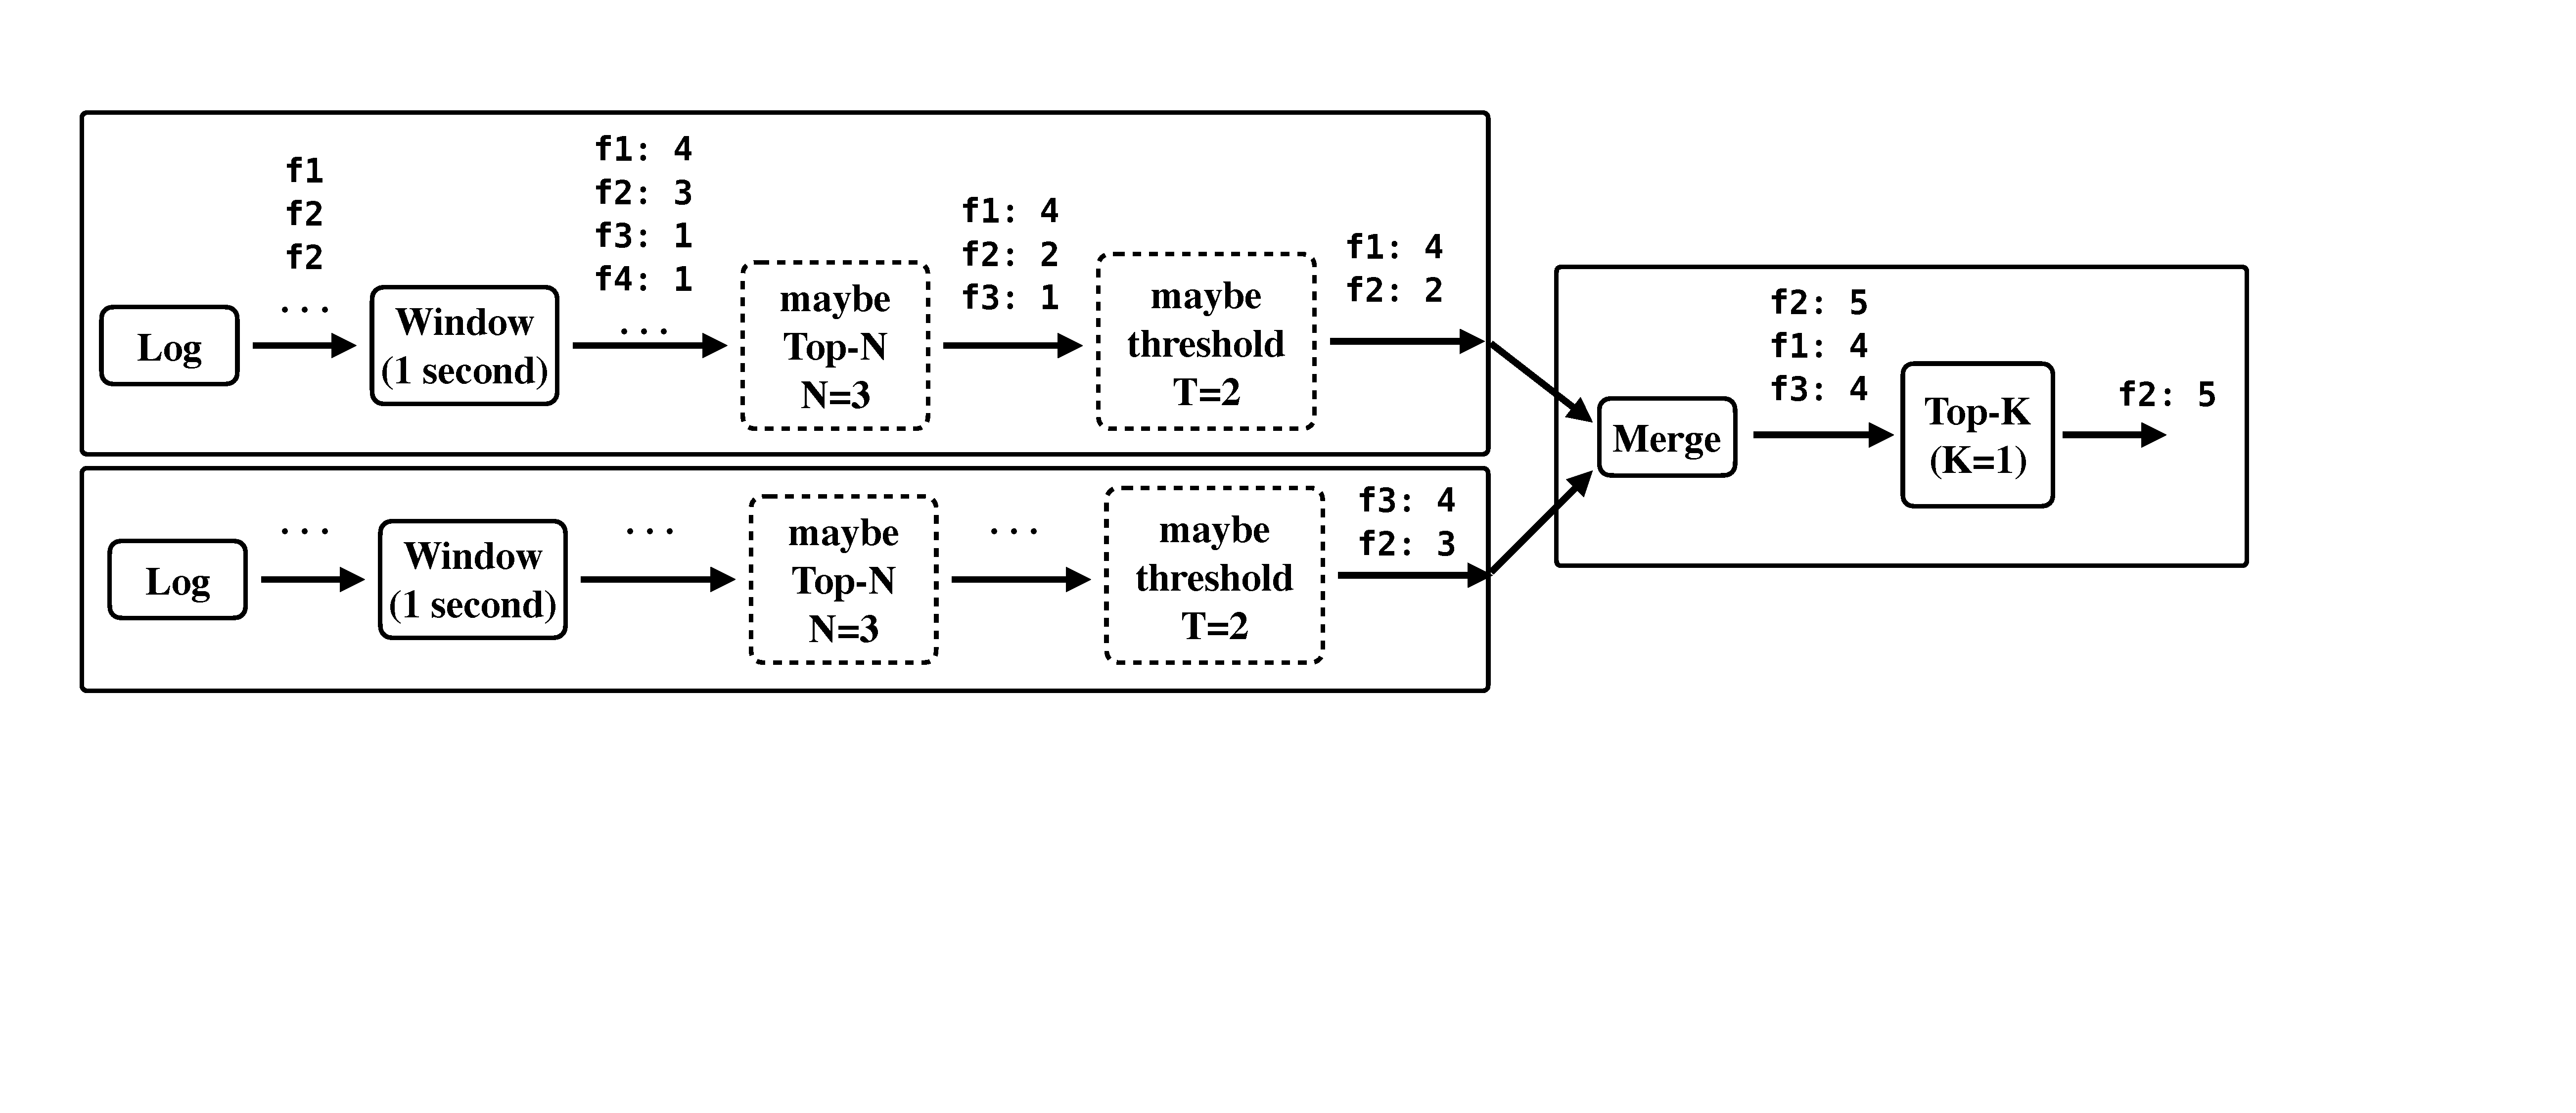
\includegraphics[width=\columnwidth]{figures/topk.pdf}
  \caption{A distributed Top-K application with two degradation operations:
    \texttt{head} and \texttt{threshold}. In this example, \texttt{f2}, which is
    not in Top-1 for either client, becomes the global Top-1 after the merge. It
    would have been purged if the clients use threshold T=3, demonstrating
    degradation that reduces data sizes affects fidelity.}
  \label{fig:topk}
  \vspace{-0.5em}
\end{figure}

\para{Distributed Top-K.} This application aggregates machine logs from
geo-distributed servers to find out the Top-K most accessed files, similar to
many Top-K queries~\cite{babcock2003distributed}.

\autoref{fig:topk} illustrates our processing pipeline with two degradation
operations. First each source node summarizes the log using \texttt{Window}
operator to reduce the data size, a pre-processing step. As many real-world
access patterns follow a long tail distribution, there can be a
large-but-irrelevant tail that contributes little to the final Top-K. Each
source node then filters the tail: (1) head(\texttt{N}) takes the top \texttt{N}
entries; (2) threshold(\texttt{T}) filters small entries whose count is smaller
than \texttt{T}. These two operations affect the final result and the exact
impact depends on data distribution. We implement these two operators by using
\sysname{}'s \maybe{} abstraction.

To measure the accuracy, we need to compare the correlation between two ranked
list. Kendall's~$\tau$~\cite{abdi2007kendall} is a correlation measure of the
concordance between two ranked list. The output ranges from \(-1\) to 1,
representing no agreement to complete agreement. To integrate with \sysname{},
we convert Kendall's~$\tau$ to [0, 1] with a linear transformation. For our
evaluation, we set K as 50 and use Apache log files that record and store user
access statistics for the \href{https://www.sec.gov}{SEC.gov} website. The logs
are split into four groups, simulating four geo-distributed nodes monitoring web
accesses. To match the load of popular web servers, we compress one hour's logs
into one second.

%%% Local Variables:
%%% mode: latex
%%% TeX-master: "../awstream"
%%% End:

%% LocalWords: runtime dataset quantization geo
\begin{figure*}[htb]
  \centering
  \begin{subfigure}[t]{0.32\textwidth}
    \centering
    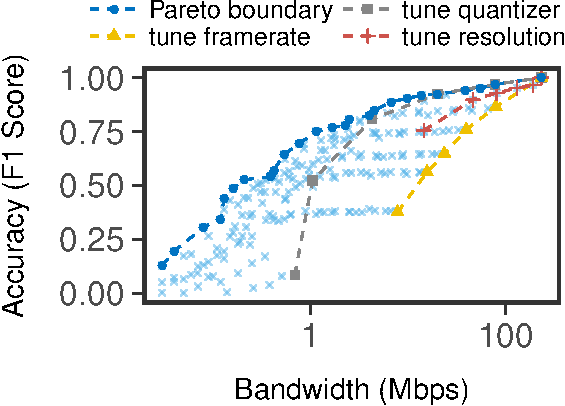
\includegraphics[width=\textwidth]{figures/profile-darknet.pdf}
    \caption{Augmented Reality (AR)}
    \label{fig:ar-profile}
  \end{subfigure}
  \hfill
  \begin{subfigure}[t]{0.32\textwidth}
    \centering
    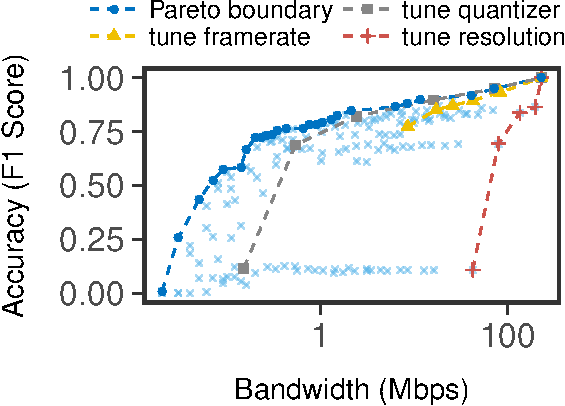
\includegraphics[width=\textwidth]{figures/profile-mot.pdf}
    \caption{Pedestrian Detection (PD)}
    \label{fig:pd-profile}
  \end{subfigure}
  \hfill
  \begin{subfigure}[t]{0.32\textwidth}
    \centering
    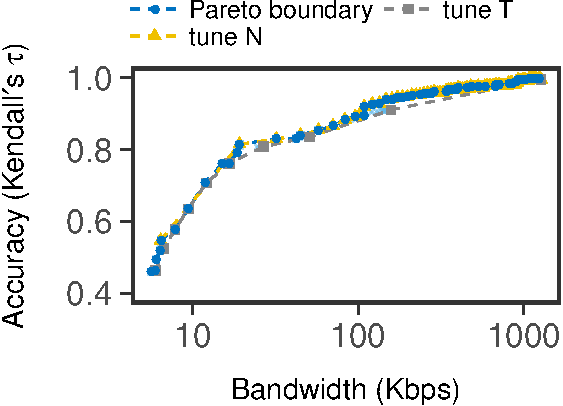
\includegraphics[width=\textwidth]{figures/profile-topk.pdf}
    \caption{Top-K (TK)}
    \label{fig:tk-profile}
  \end{subfigure}
  \caption{Application profiles of three applications. Each cross point is one
    configuration $c$'s performance $(B(c), A(c))$. All figures show the Pareto
    boundary as well as the performance if only tuning one dimension. Note the
    x-axis is in log scale.}
  \label{fig:all-profiles}
\end{figure*}

\section{Evaluation}
\label{sec:evaluation}

In this section, we show the evaluations of \sysname{}, summarizing the results
as follows.

\begin{itemize}[itemsep=0pt, topsep=3pt]
\item[\autoref{sec:application-profiles}] \sysname{} generates Pareto-optimal
  profiles across multiple dimensions with precision
  (\autoref{fig:all-profiles}).
\item[\autoref{sec:online-profiling}] Our parallel and sampling techniques
  speeds up offline and online profiling (\autoref{fig:parallel},
  \autoref{fig:online-tricks}).
\item[\autoref{sec:runtime-adaptation}] At runtime, \sysname{} achieves
  sub-second latency and nominal accuracy drop for all applications
  (\autoref{fig:ar-runtime}, \autoref{fig:pd-tk}) and across various network
  conditions (\autoref{fig:ar-rtt}).
\item[\autoref{sec:multi-task-alloc}] \sysname{} profiles allow different
  resource allocations: resource fairness and utility fairness
  (\autoref{fig:multitask}).
\end{itemize}

\subsection{Application Profiles}
\label{sec:application-profiles}

We run offline profiling using the training dataset described
in~\autoref{tab:apps} and show the learned profiles in
\autoref{fig:all-profiles}. In each figure, the cross dots represent the
bandwidth demand and application accuracy for one configuration. We highlight
the Pareto-optimal boundary $\mathbb{P}$ with blue dashed lines. To understand
each dimension's impact on the degradation, we highlight configurations from
tuning only \textit{one} dimension. From these profiles, we make the following
observations:

\para{Large bandwidth variation.} For all three applications, The bandwidth
requirements of all three applications have two to three orders of magnitude of
difference (note the x-axis is in log scale). For AR and PD, the most expensive
configuration transmits videos at 1920x1080, 30 FPS and 0 quantization; it
consumes \SI{230}{Mbps}. In contrast to the large bandwidth variation, there is
a smaller variation in accuracy. In PD, for example, even after the bandwidth
reduces to \SI{1}{Mbps} (less than 1\% of the maximum), the accuracy is still
above 75\%. The large variation allows \sysname{} to operate at a high accuracy
configuration even under severe network deterioration.

\para{Distinct effects by each dimension.} Comparing dashed lines in each
profile, we see that the Pareto-optimal configurations are only achievable when
multiple knobs are in effect. Tuning only one dimension often leads to
sub-optimal performance. Within a single profile, the difference between tuning
individual dimensions is evident. For PD, tuning resolution (the red line) leads
to a quicker accuracy drop than tuning frame rate (the yellow line). Comparing
AR and PD, the same dimension has different impact. Tuning resolution is less
harmful in AR than PD; while tuning frame rate hurts AR more than PD\@. This
echoes our initial observation in~\autoref{subsec:motivation} that
application-specific optimizations do not generalize.

% \para{Quantification with precision}. The generated profiles are actionable
% configurations that control the knobs with precision. For example, if PD
% transmits video at 1920x1080 resolution, \(10~\text{FPS}\) and a quantization
% of 20, it will consume 11.7 mbps of bandwidth, achieving roughly 90\%
% accuracy. This saves developers from laboriously analyzing their application
% to compute manual policies.

\subsection{Profiling Efficiency \& Online Profiling}
\label{sec:online-profiling}

This section focuses on the AR application as a case study; our profiling
techniques---parallelism and sampling---do not make assumptions about the
application; therefore, the evaluation results can be generalized to other
applications.

In AR, there are 216 different configurations: 6 resolutions, 6 frame rates and
6 quantization levels. AR uses YOLO~\cite{redmon2016yolo9000}, a neural network
model for object detection. It takes roughly \SI{30}{\ms} to process one frame
on GeForce\textregistered\space GTX 970.\footnote{YOLO resizes images to fixed
  416$\times$416 resolutions as required by the neural network. Evaluating
  images with different resolutions takes similar time.}  But different
configurations require different times for processing. For example, a
\(10~\text{FPS}\) video has 1/3 of the frames to process in comparison to a
\(30~\text{FPS}\) video.  In our experiment, to evaluate all 216 configurations,
it takes 52 seconds for 1 second worth of data. We denote such overhead as
52X\@. \hyperref[sec:automatic-profiling]{Section 3.2} discusses parallel and
sampling techniques to improve the profiling efficiency; we present their
evaluations as follows.

\begin{figure}
  \centering
  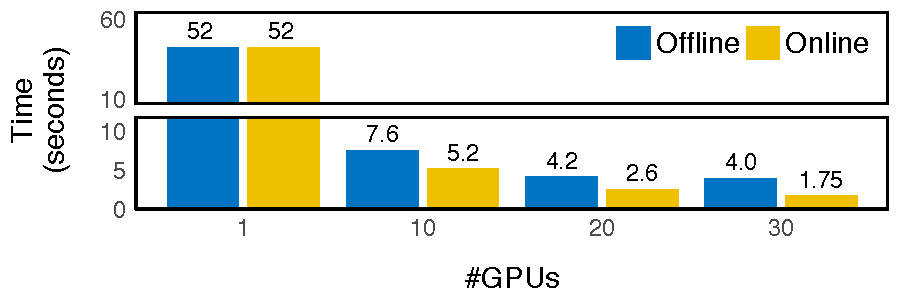
\includegraphics[width=1.0\columnwidth]{figures/parallel.pdf}
  \vspace{-1em}
  \caption{Parallelism speeds up both offline and online profiling.  The y-axis
    shows the profiling time for 1-second video.}
  \label{fig:parallel}
  \vspace{-0.5em}
\end{figure}

\para{Parallelism reduces the profiling time (\autoref{fig:parallel})}. Because
evaluating each individual configuration is independent of other configurations,
we parallelize the profiling task by assigning configurations to GPUs.
$(i)$~Our offline profiling assigns configurations randomly.  With the increased
number of GPUs, the overhead reduces from 52X to 4X with 30 GPUs.  $(ii)$~Our
online profiling assigns configurations based on the processing times collected
during offline.  \sysname{} uses LFS~\cite{karger2010scheduling} to minimize the
makespan and reduces the overhead to 1.75X with 30 GPUs (29$\times$ gain).

\para{Sampling techniques speed up online profiling
  (\autoref{fig:online-tricks}).}  Before we evaluate the speed up, we validate
\textit{model drift} with real-world data. When using the profile trained in an
office environment, the application should use a configuration of 1280x720,
\SI{30}{FPS} and 20 quantization to meet an \SI{11}{Mbps} goal. We test it
against a home environment; but at about t=100s, the camera points out of the
window to detect objects on the street. Because of the scene change, the
configuration fails to predict bandwidth, as illustrated in
\autoref{fig:offline}.

To correct the profile, if we continuously run the profiling online and update
the profile, the application will choose the right configuration to meet the
bandwidth limit.  \autoref{fig:online} shows the bandwidth prediction when we
continuously profile with the past 30 seconds of video. At time t=120s, the new
prediction corrects the drift. The downside of continuous profiling, as
discussed earlier, is the cost: 52X overhead with 1 GPU\@. In addition to
parallelism, \sysname{} uses sampling techniques for online profiling
(improvements in \autoref{tab:online}):

(i) Partial data. Instead of using all the past data, we run profiling with only
a fraction of the raw data.  \autoref{fig:online-partial} shows the bandwidth
consumption if the profiling uses only 10 seconds of data out of the past 30
seconds. In this way, although the profile may be less accurate (the
mis-prediction at t=80-100s), and there is a delay in reacting to data change
(the mis-prediction is corrected after t=125s), we save the online profiling by
3$\times$ (from 52X to 17X).

(ii) Partial configurations. If we use the past profile as a reference and only
measure a subset of $\mathbb{P}$, the savings can be substantial. A full
profiling is only triggered if there is a significant
difference. \autoref{fig:online-trigger} shows the bandwidth prediction if we
evaluate 5 configurations continuously and trigger a full profiling when the
bandwidth estimation is off by \SI{1}{Mbps} or the accuracy is off by 10\%.  For
our test data, this scheme is enough to correct model drifts by predicting an
accurate bandwidth usage (compare \autoref{fig:online} and
\autoref{fig:online-trigger}).  The overhead reduces to 6X because we run full
profiling less often (only two full profiling). It is an 8.7$\times$ gain.

\begin{figure}
  \centering
  \begin{subfigure}[t]{0.45\columnwidth}
    \centering
    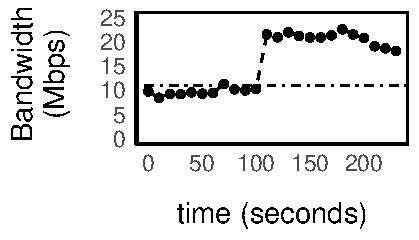
\includegraphics[width=\textwidth]{figures/online1.pdf}
    \caption{Offline only}
    \label{fig:offline}
  \end{subfigure}
  \hfill
  \begin{subfigure}[t]{0.45\columnwidth}
    \centering
    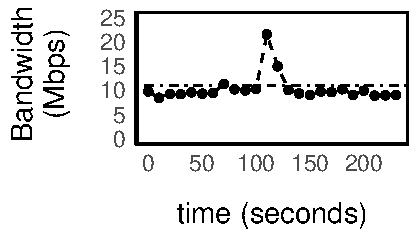
\includegraphics[width=\textwidth]{figures/online2.pdf}
    \caption{Online (continuous)}
    \label{fig:online}
  \end{subfigure}
  \\
  \vspace{0.5em}
  \begin{subfigure}[t]{0.45\columnwidth}
    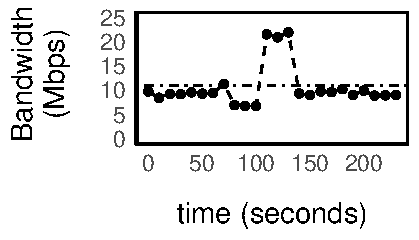
\includegraphics[width=\textwidth]{figures/online3.pdf}
    \caption{Partial data}
    \label{fig:online-partial}
  \end{subfigure}
  \hfill
  \begin{subfigure}[t]{0.45\columnwidth}
    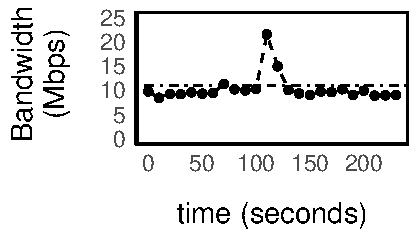
\includegraphics[width=\textwidth]{figures/online4.pdf}
    \caption{Partial configurations}
    \label{fig:online-trigger}
  \end{subfigure}
  \caption{The horizontal reference line is the target bandwidth
    (\SI{11}{Mbps}). (1) Online profiling is necessary to handle model drift
    ((a) vs.\,(b-d)). (2) Sampling techniques---partial data (c) and partial
    configurations (d)---can correct model drift with less profiling overhead
    (see \autoref{tab:online}), compared to continuous (b).  We omit accuracy
    predictions since in all schemes \sysname{} finds configurations that
    achieve similarly high accuracy (\textasciitilde 90\%).  }
  \label{fig:online-tricks}
  \vspace{-0.5em}
\end{figure}

%% Offline: 0
%% Online: 1 frame (1852.21 GPU * seconds)
%% Online (1/10)   (185.2 GPU * seconds)
%% Trigger         ( GPU * seconds)

Note that these techniques---parallelization, sampling data, and sampling
configurations---can be combined to further reduce the profiling overhead. For
example, scheduling 5 GPUs running 5 configurations continuously to check for
model drift will reduce the overhead to 1X\@. In practice, the amount of
resources to use depends on the budget and the importance of the job. \sysname{}
currently requires developers to configure the application with proper online
profiling techniques.

%% Note that it is not always needed to do online profiling. PD's test data
%% doesn't exhibit model drift.  Nor is online profiling always
%% expensive. Processing TK over all configurations.

\begin{table}[t]
  \small
  \centering
  \begin{tabular}{c c c}
    \toprule
    Online scheme & Overhead & Improvements \\
    \midrule
    Continuous & 52X & Baseline \\
    Partial data & 17X & 3$\times$\\
    Partial configurations & 6X & 8.7$\times$ \\
    \bottomrule
  \end{tabular}
  \vspace{0.5em}
  \caption{Compared to the continuous profiling baseline (52X overhead), our
    sampling techniques speed up by 3$\times$ or 8.7$\times$.}
  \label{tab:online}
  \vspace{-1em}
\end{table}

\subsection{Runtime Adaptation}
\label{sec:runtime-adaptation}

In this section, we evaluate the runtime performance by controlling bandwidth
across geo-distributed sites and compare \sysname{} with baselines including
streaming over TCP/UDP, JetStream, and video streaming. Due to limited space, we
discuss AR in depth and only present the results of PD/TK.

\para{Experiment setup.} We conduct our experiments on four geo-distributed
machines from Amazon EC2, spanning four different regions. Three (at
N.\,Virginia, Ohio, Oregon) act as worker nodes and one (at N.\,California) acts
as the analytics server. The average RTTs from the workers to the server are
\SI{65.2}{\ms}, \SI{22.2}{\ms}, and \SI{50.3}{ms}.

During the experiment, each worker transmits test data (\autoref{tab:apps}) for
about 10 mins. If the duration of the test data is less than 10 mins, it
loops. Because $B(c_{\max})$ is prohibitively large (raw videos consumes
\SI{230}{Mbps}), we use a reasonable configuration to limit the maximum rate. In
our AR experiment, $c_{\max}$ is 1600x900 resolution, \(30~\text{FPS}\) and 20
quantization; it consumes about \SI{14}{Mbps}.

Our bandwidth control scheme follows JetStream~\cite{rabkin2014aggregation}.
During the experiment, we use the Linux \texttt{tc} utility with HTB~\cite{htb,
  lartc} to control the clients' outgoing bandwidth. Each experiment involves
four phases: $(i)$~before t=200s, there is no shaping; $(ii)$~at t=200s, we
limit the bandwidth to \SI{7.5}{Mbps} for 3 minutes; $(iii)$~at t=380s, we
further decrease the bandwidth to \SI{5}{Mbps}; $(iv)$~at t=440s, we remove all
traffic shaping. For UDP, HTB doesn't emulate the packet loss or out-of-order
delivery; so we use \texttt{netem} and configure the loss probability according
to the delivery rate. Because each pair-wise connection has a different
capacity, we impose a \textit{background} bandwidth limit---\SI{25}{Mbps}---to
normalize the capacity.

We compare \sysname{} with the following baselines:

\begin{itemize}[noitemsep, nolistsep, leftmargin=*]

\item Streaming over TCP/UDP (non-adaptive). For TCP, we re-use \sysname{}
  runtime that runs over TCP but disable the adaptation. For UDP, we use
  FFmpeg~\cite{bellard2012ffmpeg} to stream video:
  RTP/UDP~\cite{schulzrinne2006rtp} for media and RTSP for
  signaling~\cite{schulzrinne1998rtsp}; as in typical video conferencing and IP
  cameras~\cite{durresi2005rtp, king2009cisco}.

\item Adaptive video streaming. We use HTTP Live Streaming (HLS) to represent
  popular adaptive video streaming techniques. Our setup resembles personalized
  live streaming systems~\cite{wang2016anatomy} but uses a smaller chunk for low
  latency (1 second instead of typical 2-10 seconds).

\item JetStream with the manual policy described in \autoref{subsec:motivation}.

\item JetStream++, a modified version of JetStream that uses the profile learned
  by \sysname{}.

\end{itemize}

At runtime, \sysname{} differs from JetStream in both policy and
adaptation. JetStream++ improves over JetStream by using our Pareto-optimal
profile. \sysname{} improves the performance further with two major changes:
$(i)$~\sysname{} directly measures the delivery rate to select an appropriate
configuration to match available bandwidth while JetStream employs a
latency-based measure of capacity ratio; $(ii)$ \sysname{} has an explicit probe
phase while JetStream changes its policy immediately after capacity ratio
changes.

\begin{figure}[t]
  \begin{subfigure}[t]{\columnwidth}
    \centering
    \includegraphics[width=0.95\columnwidth]{figures/runtime_darknet-timeseries.pdf}
    \caption{Time-series plot of the runtime behaviors: throughput (top),
      showing the effect of bandwidth shaping; latency (middle) in log scale;
      and accuracy (bottom). Overlapped lines may be hard to read; we present
      the same results in \autoref{fig:ar-runtime-boxplot} for clarity.}
    \label{fig:ar-runtime-timeseries}
  \end{subfigure}
  \vspace{0.2em}
  \\
  \begin{subfigure}[t]{\columnwidth}
    \centering
    \includegraphics[width=\columnwidth]{figures/runtime_darknet-boxplot.pdf}
    \caption{Latency and accuracy during the traffic shaping
      (i.e.,~t=200s--440s).}
    \label{fig:ar-runtime-boxplot}
  \end{subfigure}
  \caption{For AR, \sysname{} simultaneously achieves low latency and high
    accuracy (accuracy has a smaller variation).}
  \label{fig:ar-runtime}
  \vspace{-0.8em}
\end{figure}

\para{Results.} \autoref{fig:ar-runtime-timeseries} shows the runtime behavior
of \sysname{} and all baselines in time series. \autoref{fig:ar-runtime-boxplot}
summarizes the latency and accuracy with box plots during bandwidth shaping
(between t=200s and t=440s).

The throughput figure (\autoref{fig:ar-runtime-timeseries}) shows the effect of
traffic shaping. During the shaping, TCP and UDP make full use of the available
bandwidth; in comparison, \sysname{}, JetStream, JetStream++, and HLS are
conservative because of adaptation (see their throughput drops). When we stop
shaping at t=440s, TCP catches up by sending all queued items as fast as
possible. JetStream also has queued items because the policy in use (with only
three rules) cannot sustain \SI{5}{Mpbs} bandwidth. \sysname{}'s throughput
increases gradually due to the explicit probing phase. HLS is the most
conservative scheme; it does not recover from degradation until t=500s.

% summary(latency)
% Time        JetStream++        JetStream            HLS
% Min.   :206.0   Min.   :  47.14   Min.   :  541.6   Min.   :3750
% 1st Qu.:264.2   1st Qu.: 331.97   1st Qu.: 1544.6   1st Qu.:4960
% Median :322.5   Median : 539.26   Median : 1732.1   Median :5438
% Mean   :322.5   Mean   : 575.11   Mean   : 3105.8   Mean   :5578
% 3rd Qu.:380.8   3rd Qu.: 771.06   3rd Qu.: 1951.0   3rd Qu.:6270
% Max.   :439.0   Max.   :1599.51   Max.   :14245.7   Max.   :7085
% Streaming over TCP Streaming over UDP    AWStream
% Min.   :   290.8   Min.   :29.73      Min.   : 42.62
% 1st Qu.: 28042.5   1st Qu.:31.51      1st Qu.: 50.59
% Median : 54315.2   Median :33.18      Median : 79.51
% Mean   : 55596.7   Mean   :33.08      Mean   :117.72
% 3rd Qu.: 81514.5   3rd Qu.:34.90      3rd Qu.:156.22
% Max.   :117780.4   Max.   :36.29      Max.   :648.08

The latency figures (both \autoref{fig:ar-runtime-timeseries} and
\autoref{fig:ar-runtime-boxplot}) show that \sysname{} is able to maintain
sub-second latency. During the traffic shaping, TCP queues items at the sender
side for up to hundreds of seconds. In contrast, UDP always transmits as fast as
possible, leading to a consistent low latency.\footnote{FFmpeg discards packets
  that miss a deadline (\SI{33}{\ms} for \SI{30}{FPS}).} HLS's latency
fluctuates around 4-5 seconds due to chunking, buffering, and network
variations, on par with recent literature~\cite{wang2016anatomy}. Both JetStream
and JetStream++ are able to adapt during traffic shaping. With a more precise
and fine-grain policy, JetStream++ achieves a lower latency (median
\SI{539}{\ms}) in comparison to JetStream (median \SI{1732}{\ms}). Because
JetStream's runtime reacts instantaneously when the congestion condition
changes, both baselines oscillate among polices during the
experiment. \sysname{} effectively addresses the oscillation with probing and
achieves a much lower latency: median \SI{118}{\ms}, 15$\times$ improvement over
JetStream and 5$\times$ improvement over JetStream++.

% summary(accuracy)
% Time        JetStream++        JetStream           HLS
% Min.   :206.0   Min.   :0.04511   Min.   :0.5714   Min.   :0.4839
% 1st Qu.:264.2   1st Qu.:0.82776   1st Qu.:0.7854   1st Qu.:0.8414
% Median :322.5   Median :0.89079   Median :0.8401   Median :0.8795
% Mean   :322.5   Mean   :0.84882   Mean   :0.8335   Mean   :0.8684
% 3rd Qu.:380.8   3rd Qu.:0.93502   3rd Qu.:0.8952   3rd Qu.:0.9222
% Max.   :439.0   Max.   :0.98947   Max.   :0.9677   Max.   :0.9712
% Streaming over TCP Streaming over UDP     AWStream
% Min.   :0.7105     Min.   :-0.015114   Min.   :0.4516
% 1st Qu.:0.8942     1st Qu.:-0.003649   1st Qu.:0.8340
% Median :0.9261     Median : 0.003017   Median :0.8851
% Mean   :0.9181     Mean   : 0.032091   Mean   :0.8692
% 3rd Qu.:0.9545     3rd Qu.: 0.009415   3rd Qu.:0.9213
% Max.   :1.0000     Max.   : 0.925875   Max.   :0.9712

The accuracy figures (both \autoref{fig:ar-runtime-timeseries} and
\autoref{fig:ar-runtime-boxplot}) show that other than UDP, most schemes are
able to maintain high accuracy. streaming over TCP always sends data at high
fidelity, achieving the highest accuracy (median 93\%), but at a cost of high
latency. JetStream uses a manual policy that are sub-optimal in comparison to
our learned profile, so its accuracy is low (median 84\%). Using Pareto-optimal
configurations, JetStream++ is able to achieve a higher accuracy (median 89\%);
but because JetStream's runtime oscillates the policy, the accuracy has a large
variation (standard deviation 14\%). In contrast, \sysname{} chooses
configurations carefully to stay in a steady state as much as possible.  It
achieves a high accuracy of 89\% with a small variation (standard deviation
7.6\%). HLS also achieves reasonable accuracy (median 87\%) because its
adaptation of tuning resolution and encoding quality is effective in
AR. However, HLS's adaptation works poorly for PD (6\% accuracy as in
\autoref{fig:pd-runtime}).

% TK latency
% Time       Streaming over TCP Streaming over UDP    AWStream
% Min.   :210.0   Min.   : 2036      Min.   :22.29      Min.   :  48.03
% 1st Qu.:251.2   1st Qu.:11438      1st Qu.:22.42      1st Qu.: 485.08
% Median :292.5   Median :21014      Median :24.78      Median : 946.45
% Mean   :292.5   Mean   :20590      Mean   :23.85      Mean   :1145.05
% 3rd Qu.:333.8   3rd Qu.:29662      3rd Qu.:24.87      3rd Qu.:1557.20
% Max.   :375.0   Max.   :39434      Max.   :24.98      Max.   :3509.99
% > summary(accuracy)
% Time       Streaming over TCP Streaming over UDP    AWStream
% Min.   :210.0   Min.   :0.9808     Min.   :0.1097     Min.   :0.9284
% 1st Qu.:251.2   1st Qu.:0.9892     1st Qu.:0.4467     1st Qu.:0.9694
% Median :292.5   Median :0.9967     Median :0.5329     Median :0.9800
% Mean   :292.5   Mean   :0.9928     Mean   :0.5236     Mean   :0.9786
% 3rd Qu.:333.8   3rd Qu.:0.9977     3rd Qu.:0.6063     3rd Qu.:0.9883
% Max.   :375.0   Max.   :0.9991     Max.   :0.7981     Max.   :0.9991

In summary, \autoref{fig:ar-runtime} shows that \sysname{} achieves low latency
and high accuracy simultaneously. We show the results \textit{during shaping} in
a different form in \autoref{fig:intro} to discuss the trade-off between
fidelity and freshness.\footnote{We obtain \autoref{fig:intro}'s app-specific
  data by feeding PD's profile to AR. We refer to JetStream as manual policies
  in \autoref{fig:intro}.}

\begin{figure}
  \centering
  \begin{subfigure}[t]{\columnwidth}
    \captionsetup[subfigure]{aboveskip=-1em}
    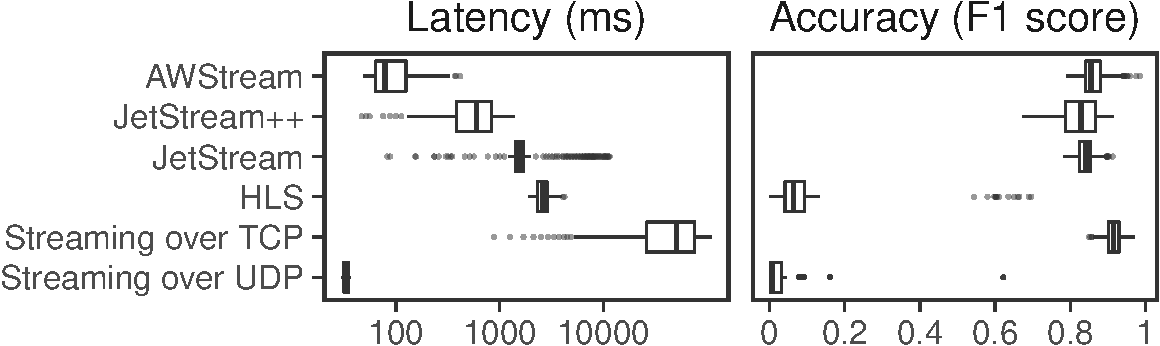
\includegraphics[width=\columnwidth]{figures/runtime_mot-boxplot.pdf}
    \begin{picture}(0,0)
      \put(-10, 80){\parbox{2cm}{\centering \caption{PD}\label{fig:pd-runtime}}}
    \end{picture}
  \end{subfigure}
  \begin{subfigure}[t]{\columnwidth}
    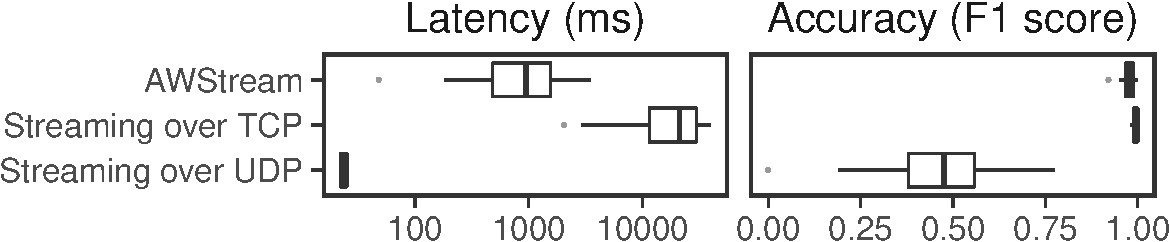
\includegraphics[width=\columnwidth]{figures/runtime_tk-boxplot.pdf}
    \begin{picture}(0,0)
      \put(-10, 60){\parbox{2cm}{\centering \caption{TK}\label{fig:tk-runtime}}}
    \end{picture}
  \end{subfigure}
  \caption{PD and TK performance summary. Box plot shows latency and accuracy
    during the traffic shaping (i.e.,~t=200s-440s).}
  \label{fig:pd-tk}
  \vspace{-1em}
\end{figure}

% \begin{figure}[t]
%   \begin{subfigure}[t]{\columnwidth}
%     \centering
%     \includegraphics[width=\columnwidth]{figures/runtime_mot-timeseries.pdf}
%     \caption{PD's runtime behavior with a time-series plot: throughput (top),
%     showing the effect of bandwidth shaping; latency (middle) in log scale;
%     and accuracy (bottom).}
%     \label{fig:pd-runtime-timeseries}
%   \end{subfigure}
%   \vspace{1em}
%   \\
%   \begin{subfigure}[t]{\columnwidth}
%     \centering
%     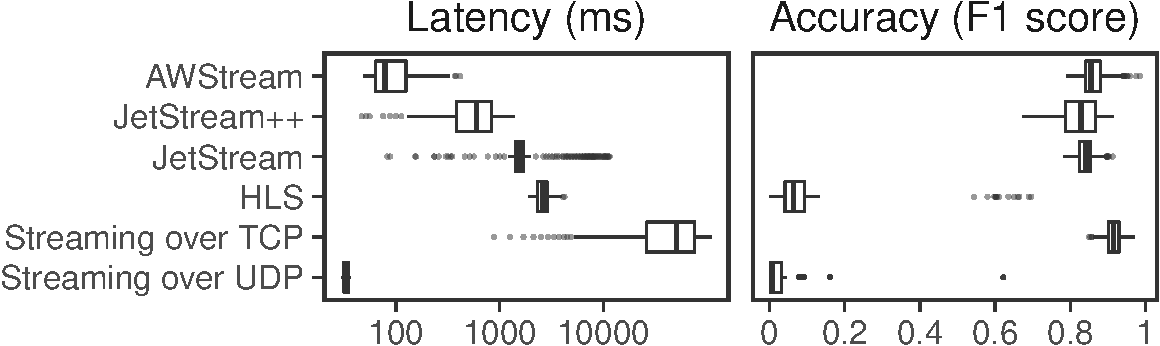
\includegraphics[width=\columnwidth]{figures/runtime_mot-boxplot.pdf}
%     \caption{PD's performance summary of latency and accuracy during the traffic
%     shaping (between t=200s and t=440s).}
%     \label{fig:pd-runtime-boxplot}
%   \end{subfigure}
%   \caption{PD runtime evaluation.}
%   \label{fig:pd-runtime}
%   \vspace{-0.5em}
% \end{figure}

% \begin{figure}[t]
%   \begin{subfigure}[t]{\columnwidth}
%     \centering
%     \includegraphics[width=\columnwidth]{figures/runtime_tk-timeseries.pdf}
%     \caption{TK's runtime behavior with a time-series plot: throughput (top),
%     showing the effect of bandwidth shaping; latency (middle) in log scale;
%     and accuracy (bottom).}
%     \label{fig:tk-runtime-timeseries}
%   \end{subfigure}
%   \vspace{1em}
%   \\
%   \begin{subfigure}[t]{\columnwidth}
%     \centering
%     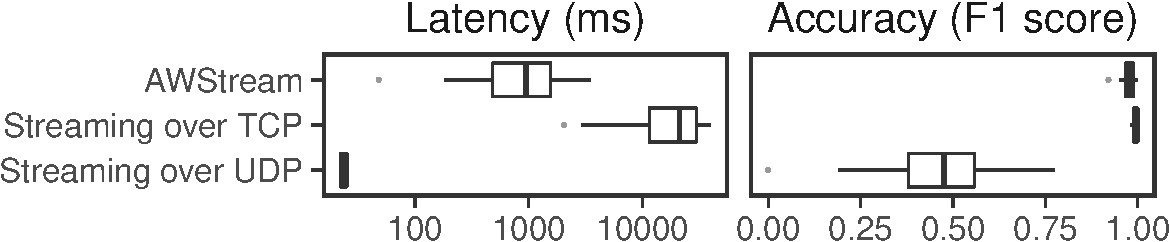
\includegraphics[width=\columnwidth]{figures/runtime_tk-boxplot.pdf}
%     \caption{TK's performance summary of latency and accuracy during the traffic
%     shaping (between t=200s and t=440s).}
%     \label{fig:tk-runtime-boxplot}
%   \end{subfigure}
%   \caption{TK runtime evaluation.}
%   \label{fig:tk-runtime}
%   \vspace{-0.5em}
% \end{figure}

\para{Pedestrian Detection.} The setup for PD is the same with AR: three clients
and one server on EC2. $c_{\max}$ is 1920x1080 resolution, \(10~\text{FPS}\) and
20 quantization; it consumes about \SI{12}{Mbps}. For PD, \sysname{} learns that
resolution is more important than frame rate. Hence it favors 1080p with 10FPS
over 900p with 30FPS. We use the same bandwidth shaping schedule and baselines
as AR. \autoref{fig:pd-runtime} shows the result and most observations about
latency/accuracy are the same as AR. HLS has a poor accuracy because it reduces
resolution and encoding quality during adaptation. \sysname{} is able to achieve
the lowest latency (\SI{78}{ms}) with small accuracy drop (86\%, 6\% drop in
comparison to TCP). In comparison to JetStream, \sysname{} improves the latency
by 20$\times$ (from \SI{1535}{ms} to \SI{78}{ms}) and accuracy by 1\% (from 84\%
to 85\%).

\para{Top-K.} For TK, we use four clients and one server because our logs are
split into four groups. $c_{\max}$ is $N=9750$ for \texttt{head} and $T=0$ for
\texttt{threshold}; it consumes about \SI{1.2}{Mbps}. Because the overall
bandwidth consumption is much smaller than video analytics, we modify the
bandwidth parameter: during t=200-380s, we limit the bandwidth to
\SI{750}{Kbps}; during t=380-440s, the bandwidth is \SI{500}{Kbps}; the
background limit is \SI{2.5}{Mpbs}. We only compared \sysname{} with streaming
over TCP and UDP. JetStream's Top-K is based on TPUT~\cite{cao2004efficient}
that targets at queries asked hourly or daily. We did not implement our Top-K
pipeline (\autoref{fig:topk}) with JetStream because video analytics suffice the
purpose of comparison. \autoref{fig:tk-runtime} shows the evaluation
results. Streaming over TCP has the highest accuracy (99.7\%) but the worst
latency (up to 40 seconds). Streaming over UDP has the lowest latency but the
worst accuracy (52\%). \sysname{} achieves low latency (1.1 seconds) and high
accuracy (98\%) simultaneously. Notice that because TK's source generates data
every second after \texttt{Window}, one object in the queue leads to one second
latency.

\vspace{0.3em}
\para{Performance with Varying Network Delays}
\vspace{0.2em}

\noindent \sysname{} targets at wide area whose key characteristic is the large
variation in latency~\cite{li2010cloudcmp}. While we have conducted experiments
using real-world setup on EC2, the latency between EC2 sites is relatively low.
To evaluate how \sysname{} performs with increased network delays, we conducted
another experiment with one pair of client and server under different network
conditions. We use \texttt{netem} to add delays, up to \SI{250}{ms} each way, so
the added RTT can be as high as \SI{500}{ms}. The delay follows a normal
distribution where the variation is 10\%, e.g.\,$250\pm 25\text{ms}$.

\begin{figure}
  \centering
  \includegraphics[width=.88\columnwidth]{figures/runtime_darknet-bench.pdf}
  \caption{\sysname{} maintains low latency and high accuracy under different
    network delay conditions.}
  \label{fig:ar-rtt}
  \vspace{-0.5em}
\end{figure}

\autoref{fig:ar-rtt} shows the runtime behavior with various added network
delays. While the latency increases with the added delay, \sysname{} mostly
manages to achieve sub-second latency for all conditions. We see a higher
variation in latency and more outliers as network delay increases, because the
congestion detection is slow when the RTT is high. In terms of accuracy, because
\sysname{} mostly stays in \texttt{Steady} state and accuracy only depends on
the level of degradation, \sysname{} achieves similar accuracy for different
network delays.

\subsection{Resource Allocation and Fairness}
\label{sec:multi-task-alloc}

\begin{figure}
  \centering
  \begin{subfigure}[t]{0.7\columnwidth}
    \centering
    
\includegraphics[width=\textwidth]{figures/multitask-legend.pdf}
  \end{subfigure}
  \\
  \vspace{0.4em}
  \begin{subfigure}[t]{0.45\columnwidth}
    \centering
    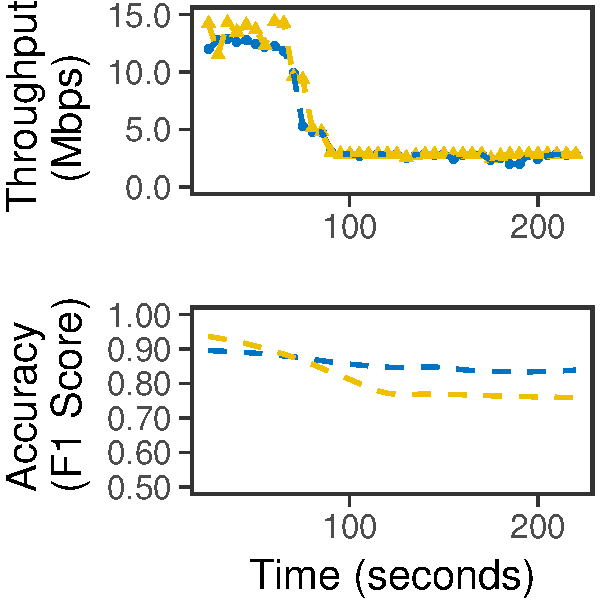
\includegraphics[width=\textwidth]{figures/multitask-left.pdf}
    \caption{Resource Fairness}
    \label{fig:eq-bw}
  \end{subfigure}
  \hfill
  \begin{subfigure}[t]{0.45\columnwidth}
    \centering
    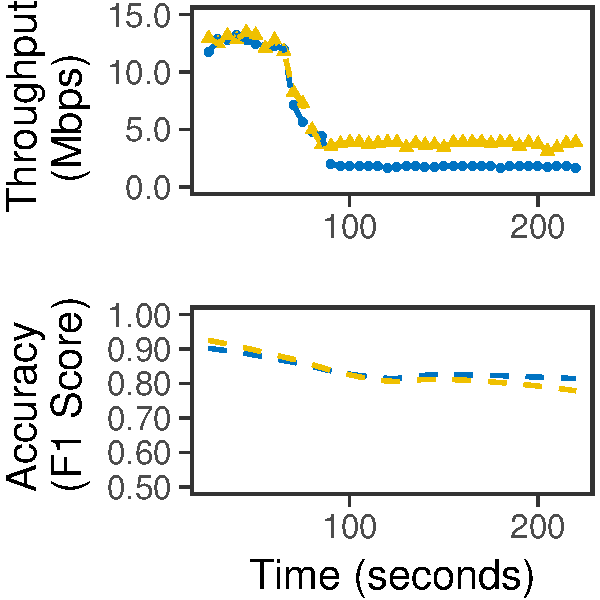
\includegraphics[width=\textwidth]{figures/multitask-right.pdf}
    \caption{Utility Fairness}
    \label{fig:eq-acc}
  \end{subfigure}
  \caption{\sysname{} allows different resource allocation schemes.}
  \label{fig:multitask}
  \vspace{-0.8em}
\end{figure}

We evaluate resource allocations with two applications. In this way, the result
also covers the case of a single application, and can generalize to more
applications.

We choose AR and PD as the example applications.  The clients and servers of
both applications are co-located so that they share the same bottleneck
link. The experiment starts with sufficient bandwidth. At t=60s, we start
traffic shaping to limit the total bandwidth to \SI{6}{Mbps}. When we allocate
resource equally between two applications (\autoref{fig:eq-bw}), each
application gets \SI{3}{Mbps}. Under this condition, PD runs with a higher
accuracy of 85\% while AR only achieves 77\%. In addition to resource fairness,
\sysname{} supports utility fairness: it chooses configurations that maximize
the minimal accuracy. In this experiment, PD receives \SI{2}{Mbps} and AR
receives \SI{4}{Mbps}; and both achieve 80\% accuracy (\autoref{fig:eq-acc}).

%%% Local Variables:
%%% mode: latex
%%% TeX-master: "../awstream"
%%% End:

%% LocalWords: TK PD runtime JetStream AR alloc YOLO dataset outliers
%% LocalWords: makespan subsec mins tcp boxplot geo HLS ffmpeg geforce
%% LocalWords: HLS PD's mis bw quantization RTSP RTP GPUs parallelization
%% LocalWords: eq netem resizes RTTs parallelize LFS UDP GTX analytics
%% LocalWords: FFmpeg GeForce HLS's JetStream's TK's tc HTB TPUT RTT
\section{Discussion and Future work}
\label{sec:discussion}

\paraf{Reducing Developer Effort.} While \sysname{} simplifies developing
adaptive applications, there are still application-specific parts required for
developers: wrapping appropriate \maybe{} calls, providing training data, and
implementing accuracy functions. Because \sysname{}'s API is extensible, we plan
to build libraries for common degradation operations and accuracy functions,
similar to machine learning libraries.

\para{Fault-tolerance and Recovery.} \sysname{} tolerates bandwidth variation
but not network partition or host failure. Although servers within data centers
can handle faults in existing systems, such as Spark
Streaming~\cite{zaharia2013discretized}, it is difficult to make edge clients
failure-oblivious.  We leave failure detection and recovery as a future work.

\para{Profile Modeling.} \sysname{} currently performs an exhaustive search when
profiling, and only use parallelism and sampling to speed up. We plan to improve
our profiler with statistical methods such as Bayesian
Optimization~\cite{snoek2012practical, alipourfard2017cherrypick} that can model
black box functions $B(c)$ and $A(c)$.

% \para{Expressiveness}: Our \maybe{} APIs allow an easy integration with
% existing stream processing systems. While it follows the operator model,
% combined with other operators, this is expressive enough. We've presented
% three applications in this paper; and we are implement more application using
% this framework to understand the expressiveness better.

% \para{Context detection.} \sysname{} is currently limited to one profile: the
% offline profiling generates the default profile and the online profiling
% updates the single profile continuously.  Real-world applications may produce
% data with a multi-modal distribution, where the model changes upon context
% changes, such as indoor versus outdoor. Therefore, one possible optimization
% to \sysname{} is to allow multiple profiles for one application, detect
% context changes, and use the profile that best matches the current data
% distribution.  Switching contexts could reduce, or even eliminate, the
% overhead of online profiling.

\para{Predicting Bandwidth Changes.} \sysname{} currently does not predict
future bandwidth. While reacting to bandwidth changes is enough to achieve
sub-second latency, we plan to improve our runtime further (e.g.\,removing
latency spikes) with techniques that can predict future resources, such as model
predictive control (MPC)~\cite{camacho2013model, yin2015control}.

%%% Local Variables:
%%% mode: latex
%%% TeX-master: "../awstream"
%%% End:

%% LocalWords: CherryPick runtime MPC QoE profiler
\section{Related Work}
\label{sec:related-work}

\paraf{JetStream.} JetStream is the first to use degradation to reduce latency
for wide-area streaming analytics. Compared to JetStream, \sysname{} makes five
major contributions: $(1)$~a novel API design to specify degradation in a simple
and composable way; $(2)$~automatic offline profiling to search for
Pareto-optimal configurations; $(3)$~online profiling to address model drift;
$(4)$~an improved runtime system achieving sub-second latency (comparison in
\autoref{sec:runtime-adaptation}); $(5)$~support for different resource
allocation policies for multiple applications.

\para{Stream Processing Systems.} Early streaming
databases~\cite{abadi2005design, chandrasekaran2003telegraphcq} have explored
the use of dataflow models with specialized operators for stream
processing. Recent research projects and open-source
systems~\cite{akidau2013millwheel, toshniwal2014storm, sanjeev2015twitter,
  zaharia2013discretized, carbone2015apache} primarily focus on fault-tolerance
in the context of a single cluster. When facing back pressure,
Storm~\cite{toshniwal2014storm}, Spark Streaming~\cite{zaharia2013discretized}
and Heron~\cite{sanjeev2015twitter} throttle data ingestion; Apache
Flink~\cite{carbone2015apache} uses edge-by-edge back-pressure techniques
similar to TCP flow control; Faucet~\cite{lattuada2016faucet} leaves the flow
control logic up to developers.  While our work has a large debt to prior
streaming work, \sysname{} targets at the wide area and explicitly explores the
trade-off between data fidelity and freshness.

\para{Approximate Analytics.} The idea of degrading computation fidelity for
responsiveness is also explored elsewhere, such as SQL
queries~\cite{hellerstein1997online, agarwal2013blinkdb,
  ananthanarayanan2014grass}, real-time processing~\cite{farrell2016meantime},
and video processing within large clusters~\cite{zhang2017live}. The trade-off
between available resource and application accuracy is a common theme among all
these systems. \sysname{} targets at wide-area streaming analytics, an emerging
application domain especially with the advent of IoT\@.

\para{WAN-Aware Systems.} Geo-distributed systems need to cope with high latency
and limited bandwidth. While some systems assume the network can prioritize a
small amount of critical data under congestion~\cite{cho2012surviving}, most
systems reduce data sizes in the first place to avoid congestion,
e.g.\,LBFS~\cite{muthitacharoen2001low}. Over the past two years, we have seen a
plethora of geo-distributed analytical frameworks~\cite{vulimiri2015wananlytics,
  vulimiri2015global, pu2015low, kloudas2015pixida, viswanathan2016clarinet}
that incorporate heterogeneous wide-area bandwidth into query optimization to
minimize data movement. While effective in speeding up analytics, these systems
focus on batch tasks such as MapReduce jobs or SQL queries. Such tasks are often
executed infrequently and without real time constrain. In contrast, \sysname{}
processes streams continuously in real time.

%% - Pixida~\cite{kloudas2015pixida} minimizes data movement across inter-DC
%% links by solving a traffic minimization problem in data analytics.

%% - Iridium~\cite{pu2015low} optimizes data and task placement jointly to
%% achieve an overall low latency goal.

%% - Clarinet~\cite{viswanathan2016clarinet} incorporate bandwidth information
%% into query optimizer to reduce data transfer.

%% WheelFS~\cite{stribling2009flexible}

%% Geode~\cite{vulimiri2015global} develops input data movement and join
%% algorithm selection strategies to minimize WAN bandwidth usage.

%% WANalytics~\cite{vulimiri2015wananlytics} focuses on batch analytics.

%% SWAG~\cite{hung2015scheduling} coordinates compute task scheduling across
%% DCs.

%% \cite{heintz2015towards} discusses the complex trade-offs involved in
%% wide-area analytics.

\para{(Adaptive) Video Streaming.} Multimedia streaming protocols,
e.g.\,RTP~\cite{schulzrinne2006rtp}, aim to be fast instead of reliable. While
they can achieve low latency, their accuracy can be poor under congestion.
Recent work has moved towards HTTP-based protocols and focused on designing
adaptation strategy to improve QoE, as in research~\cite{mao2017neural,
  sun2016cs2p, yin2015control} and industry (HLS~\cite{pantos2016http},
DASH~\cite{michalos2012dynamic, sodagar2011mpeg}). These adaptation strategies
are often pull-based: client keeps checking the index file for changes. And
clients have to wait for the next chunk (typically 2-10 seconds). In addition,
as we have shown in \autoref{sec:runtime-adaptation}, their adaptation is a poor
match for analytics that rely on image details (e.g.\,6\% accuracy for PD). In
contrast, \sysname{} learns an adaptation strategy for each application (also
not limited to video analytics); and the runtime is optimized for low latency.

\para{QoS.} Most QoS work~\cite{ferrari1990scheme, shenker1994integrated,
  shenker1995fundamental} in the 1990s focuses on network-layer solutions that
are not widely deployable. \sysname{} adopts an end-host application-layer
approach ready today for WAN. For other application-layer
approaches~\cite{vandalore2001survey}, \sysname{}'s API can incorporate their
techniques, such as encoding the number of layers as a knob to realize the
layered approach in Rejaie et al~\cite{rejaie2000layered}. Fundamentally,
\sysname{} does not provide hard QoS guarantees; instead \sysname{} maximizes
achievable accuracy (application performance) and minimizes latency (system
performance) with respect to bandwidth constraints: a multidimensional
optimization.

%% TCP, for example, adapts to available bandwidth by controlling the congestion
%% window with AIMD~\cite{jacobson1988congestion}.  Previous work has proposed
%% modifications to TCP for specific contexts. For streaming over TCP, Goel et
%% al.~\cite{goel2008low} proposes adaptive buffer-size tuning. For the cloud,
%% Adaptive TCP~\cite{wu2013adaptive} proposes to modify the congestion control
%% behavior based on flow size for the cloud.

% \para{Scheduling and allocation:} Resource allocations in the cloud is how to
% efficiently allocate tasks.  In the wide area, we face fundamental limit that
% therefore degradation is more effective. For multiple tasks, Existing
% allocations are for resources without considering application trade-offs.
% MediaNet~\cite{hicks2003user} uses both local and online global resource
% scheduling to improve user performance and network utilization, and adapts
% without requiring underlying support for resource
% reservations. VideoStorm~\cite{zhang2017live} primarily focuses on cluster
% resource allocation among video queries. For wide-area, the resource
% allocation is limited. We do not control the capacity; but still we can
% allocate the available bandwidth.

% Performance modeling: CherryPick~\cite{alipourfard2017cherrypick},
% Ernest~\cite{venkataraman2016ernest}.
%% Dolly~\cite{ananthanarayanan2013effective}.
%% \para{Program Synthesis:}

%%% Local Variables:
%%% mode: latex
%%% TeX-master: "../awstream"
%%% End:

%% LocalWords: JetStream analytics composable runtime Borealis TelegraphCQ
%% LocalWords: dataflow MillWheel Flink TCP BlinkDB VideoStorm IoT geo LBFS
%% LocalWords: WANalytics Pixida MapReduce RTP HLS QoE VoD QoS deployable Rejaie
%% LocalWords: et al

\section{Conclusion}
\label{sec:conclusion}

This paper presents \sysname{}, a stream processing system for a wide variety of
applications by enabling developers to customize degradation operations with
\maybe{} operators. Our automatic profiling tool generates an accurate profile
that characterizes the trade-off between bandwidth consumption and application
accuracy. The profile allows the runtime to react with precision. Evaluations
with three applications show that \sysname{} achieves sub-second latency with
nominal accuracy drop. \sysname{} enables resilient execution of wide-area
streaming analytics with minimal developer effort.

%%% Local Variables:
%%% mode: latex
%%% TeX-master: "../../thesis"
%%% End:

%% LocalWords: analytics runtime

%%% Local Variables:
%%% mode: latex
%%% TeX-master: "../thesis"
%%% End:

% \chapter{Compute Resource Adaptation}
\label{cha:comp-reso-adapt}

This chapter features BRT.

\section{Introduction}
\label{sec:introduction}

\para{App flourish}. Mobile and Internet of Things (IoT) applications---such as
Microsoft SeeingAI~\cite{seeingai} and Google
Assistant~\cite{googleassistant}---are increasingly powered by machine learning
for daily tasks. These applications perform the \textit{inference} step of
machine learning: they use trained models to make a prediction given an input,
such as visual~\cite{googlelens, ha2014towards, seeingai}, audio~\cite{alexa,
  applesiri, cortana}, and sensory information~\cite{laput2017synthetic,
  lu2010jigsaw}. While there is a staggering collection of research focusing on
model \textit{training}, model deployment and prediction serving has received
relatively little attention.  In this paper, we study prediction serving for
wide-area mobile/IoT applications.

\para{Challenge to provide consistent low latency (sub-second) response}. Low
latency serving is important for smooth user experience. Previous
studies~\cite{nielsen1994usability, schneiderman1998designing} have measured the
effect of different end-to-end latencies: 100 ms gives the feeling of
instantaneous response, 1 second keeps the user's flow of thought seamless, and
a few seconds' delay creates an unpleasant user experience.

%% Reference:
%% https://www.nngroup.com/articles/website-response-times/

%% 0.1 seconds gives the feeling of instantaneous response — that is, the
%% outcome feels like it was caused by the user, not the computer. This level of
%% responsiveness is essential to support the feeling of direct manipulation
%% (direct manipulation is one of the key GUI techniques to increase user
%% engagement and control — for more about it, see our User Interface Principles
%% Every Designer Must Know course).

%% 1 second keeps the user's flow of thought seamless. Users can sense a delay,
%% and thus know the computer is generating the outcome, but they still feel in
%% control of the overall experience and that they're moving freely rather than
%% waiting on the computer. This degree of responsiveness is needed for good
%% navigation.

%% 10 seconds keeps the user's attention. From 1–10 seconds, users definitely
%% feel at the mercy of the computer and wish it was faster, but they can handle
%% it.

%% There are also some great discussion about latency here:
%% https://danluu.com/term-latency/

%% More examples: Wearable cognitive assistant~\cite{ha2014towards} that uses
%% wearable devices, such as Google Glass, for deep cognitive assistance (e.g.,
%% offering hints for social interaction via real-time scene analysis).
%% SeeingAI is a talking camera for the blind and low vision community that
%% describes nearby people, text, objects. \xin{Google lens
%% (https://36kr.com/p/5075676.html).  Siri, Google assistant, Amazon Alexa
%% (Echo).}

\para{Why challenging? Discrepancy in performance, shared network/service.}
Meeting sub-second latency goals consistently has remained challenging,
especially for complex prediction servings beyond the capabilities of end
devices. State-of-the-art computer vision algorithms, such as object detection,
easily take several seconds on modern smartphones~\cite{chen2015glimpse}. Prior
work explores offloading to the cloud or the edge\footnote{Also referred to as
  cloudlet~\cite{satyanarayanan2009case}, the fog~\cite{bonomi2012fog}.}  that
hosts machine learning models and serves predictions. Despite their powerful
computing capability and more available resources---including special hardware
like GPU and TPU~\cite{jouppi2017datacenter}---these platforms suffer from
increased network latency and service overload, thus unable to meet latency
goals consistently. We illustrate the spectrum of resources, workload and
latency among end devices, the edge and the cloud in
\autoref{fig:mobile-edge-cloud}.

%% Existing systems~\cite{crankshaw2017clipper, yun2015optimal} strives to bound
%% tail performance to meet service level objectives (SLO).

\begin{figure}
  \centering
  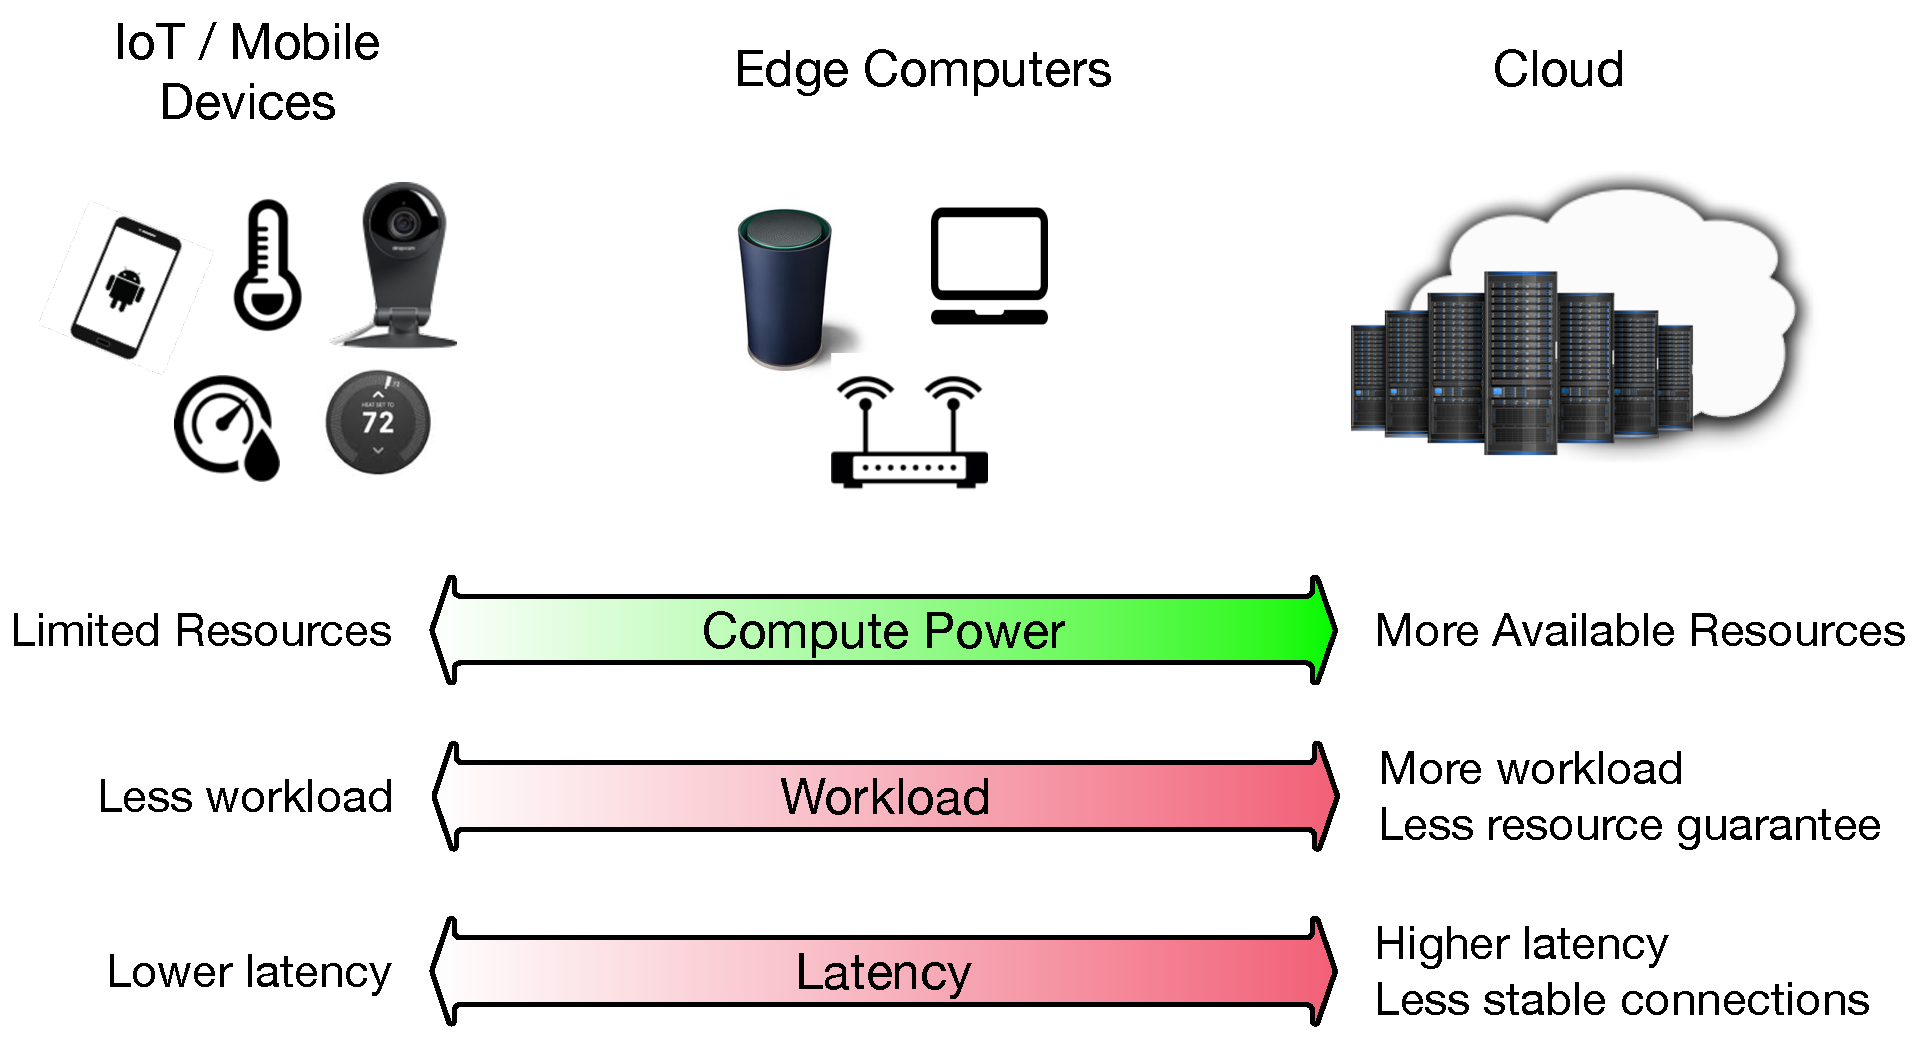
\includegraphics[width=0.95\columnwidth]{figures/background.pdf}
  \caption{Characteristics of IoT/mobile, edge and cloud.}
  \label{fig:mobile-edge-cloud}
\end{figure}

This paper presents \sysname{}, a general prediction serving framework that
provides bounded response times for IoT. Its core is about performance modeling
by exploring the tradeoff space between application accuracy and cost
(processing times). Orthogonal to existing system solutions with scale-out,
scale-up, caching or batching, \sysname{} requires knowledge from the
application.

\para{(short) Accuracy-Cost Tradeoff.} For a particular inference task, multiple
algorithms or tunable parameters for one algorithm exist that requires different
processing times and result in different accuracy. To accommodate the
resource-constrained devices, one can use an algorithm or a parameter that suits
the particular platform. In order to explore the trade-off space, \sysname{}
takes a data-driven approach to learn the relationship between inference
accuracy and processing times for each algorithm and different parameters for
individual platforms. We call this process ``profiling'' and its goal is to find
Pareto-optimal configurations (algorithm and parameter) as the performance
model. Profiling with an exhaustive search may not be feasible for some
algorithms due to their large parameter space. In these cases, \sysname{} uses a
statistical method, Bayesian Optimization (BO), to model the relationship as a
black-box function and only searches for near-optimal configurations.

\para{(short) Ensemble of Machines.} While running a low accuracy configuration
on end devices ensures bounded latency, the accuracy may not be
satisfactory. \sysname{} improves the accuracy by combining available resources
such as the edge and the cloud, similar to existing techniques such as
offloading~\cite{chun2011clonecloud,cuervo2010maui} and redundant
requests~\cite{ananthanarayanan2013effective, dean2013tail,
  gordon2015accelerating, vulimiri2013low}. One key difference between
\sysname{} and existing approaches is that \sysname{} uses the learned
performance model to find platform-specific configurations instead of running
the same computation (\autoref{fig:dr}).

\begin{figure}
  \centering
  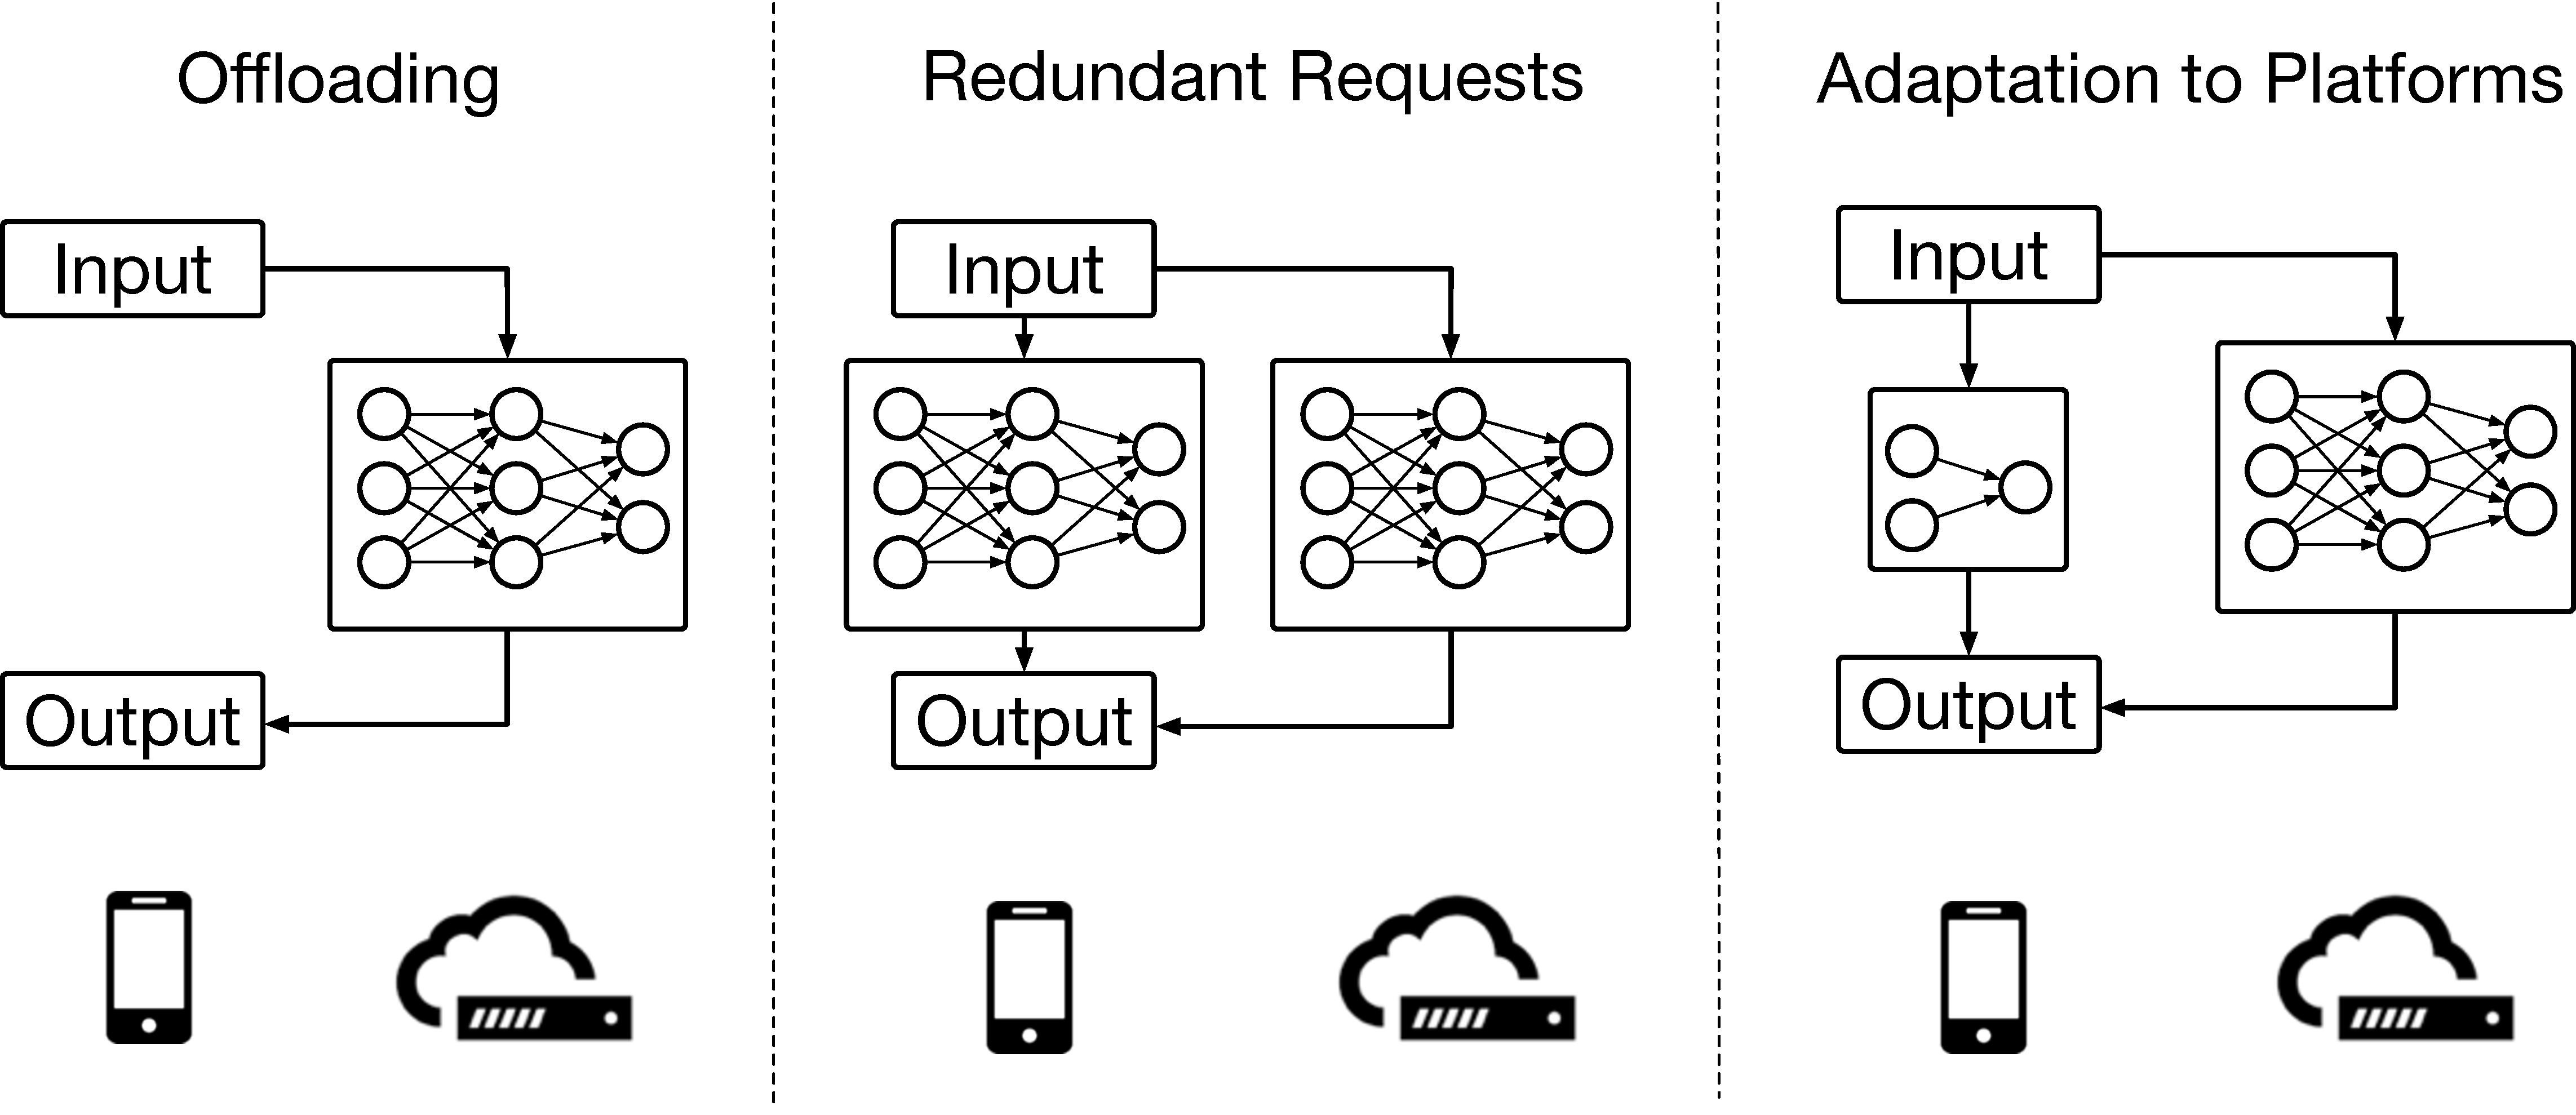
\includegraphics[width=\columnwidth]{figures/dr.pdf}
  \caption{Illustration of offloading, redundant requests and differential
    redundancy.}
  \label{fig:dr}
\end{figure}

We call this differential differential redundancy (DR) and illustrate the idea
using face detection as an example. For a particular image, a less power
platform, such as the mobile, can reduce the image resolution to speed up
detection. As a result, it only detects large faces, offering an
inaccurate-but-fast response. At the same time, a redundant request is sent to a
powerful server. The server can detect all tiny faces, yielding a higher
accuracy. The result is then returned and merged with the initial result. From
the user's perspective, face detection is \emph{instantaneous} and gradually
\emph{accurate}.

To make DR effective and efficient, \sysname{} should utilize available
resources but avoid sending unnecessary requests. We treat the as a multi-armed
bandit problem and model the uncertainty behind network delays and service
contention. When the uncertainty grows, it favors redundant requests
(exploration); if there is an apparent winner among all dispatching options, it
avoids excessive service requests (exploitation).

\para{(short) SLO-aware scheduling.} Each request is annotated with a
service-level objective (SLO) that describes the deadline and accuracy
demand. Upon receiving a request, the server runs a real-time scheduler to meet
all SLOs. Existing real-time scheduler often assumes a worst-case execution time
(WCET) and runs earliest deadline first (EDF) schedule. Our scheduler has two
key differences when trying to meet SLOs: $(i)$ \sysname{} can adjust each
request's serving time and quality based on the profile; $(ii)$ \sysname{} is
allowed to reject a request because of the redundancy mentioned above.

At runtime, when a request comes in, the server first performs triage to
determine the urgency of the request and its priority among all pending
tasks. If all tasks are still schedulable after admitting the new request, it's
added to the task queue; otherwise, \sysname{} rejects the request. The
schedulability is checked if all requests are serviced at its lowest-allowed
quality; this allows us to reject fast by only keeping track of available
\texttt{capacity}. When performing the actual scheduling, \sysname{} can spare
the remaining capacity to increase some tasks' quality. Our scheduler is
non-preemptive and treat all requests equally.

We've implemented the aforementioned techniques and evaluated their
effectiveness over three applications. We make the following contributions with
\sysname{}:

\begin{itemize}[leftmargin=*, topsep=0pt, itemsep=0pt]

\item Performance modeling. We cast the performance modeling as multi-objective
  optimization problems. Our BO-based profiling can effectively explore the
  large parameter space and finds near-optimal solutions.

\item Differential redundancy. For prediction serving, we propose to use perform
  redundant servings with different algorithms and parameters for each platform
  to harness the heterogeneity.

\item Runtime dispatch. During the runtime dispatch, we model the online
  scheduler as a multi-armed bandit problem with budget constrain. Our scheduler
  is able to save 30\% energy over baseline schedulers.

\item Server triage. The server continuously adjusts the priority of each
  requests to maximize throughput while meeting SLOs.

\end{itemize}

% \begin{figure*}
%   \centering
%   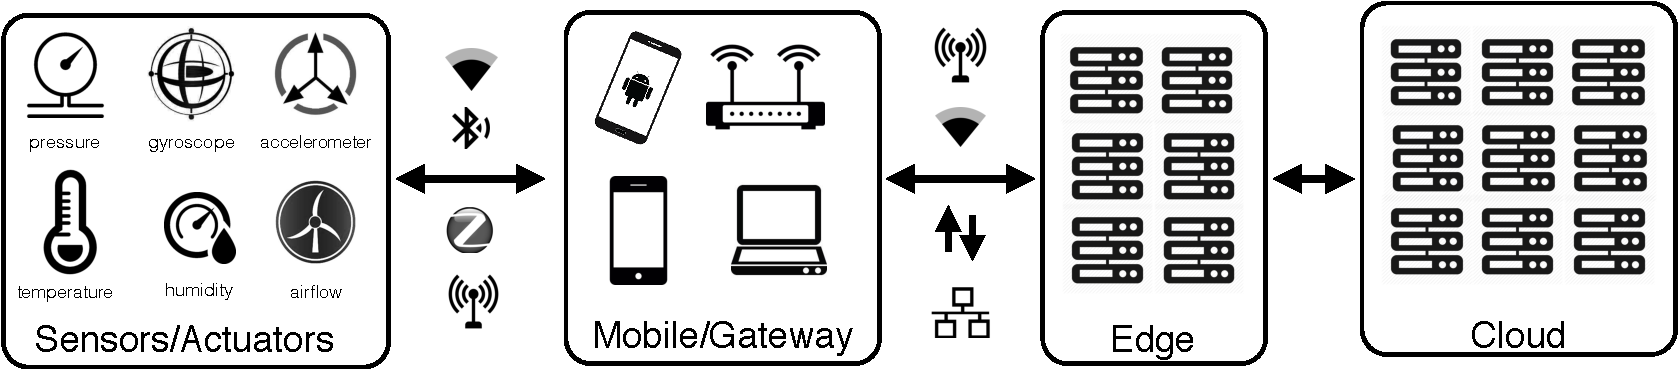
\includegraphics[width=\textwidth]{figures/platforms}
%   \label{fig:options}
%   \caption{Platforms}
% \end{figure*}

%%% Local Variables:
%%% mode: latex
%%% TeX-master: "../../thesis"
%%% End:

\newpage
\section{Applications and Challenges}
\label{sec:motivation}

We focus on computation-heavy ML applications that is beyond the capability of
local devices. Offer some concrete numbers here. Mention that many approaches in
application domains are improving accuracy at a cost of increased
computation. And the spectrum of accuracy-cost is common in these applications.

Also describe application benchmark data set here.

For Face, we use FDDB dataset.

\subsection{Challenges}
\label{sec:challenges}

Motivated by the above applications, we outline the key challenges of exploiting
accuracy-cost trade-off for prediction serving and describe how \sysname{}
addresses these challenges.

\subsubsection*{Heterogeneous Environment}

% \begin{figure}[t]
%   \centering
%   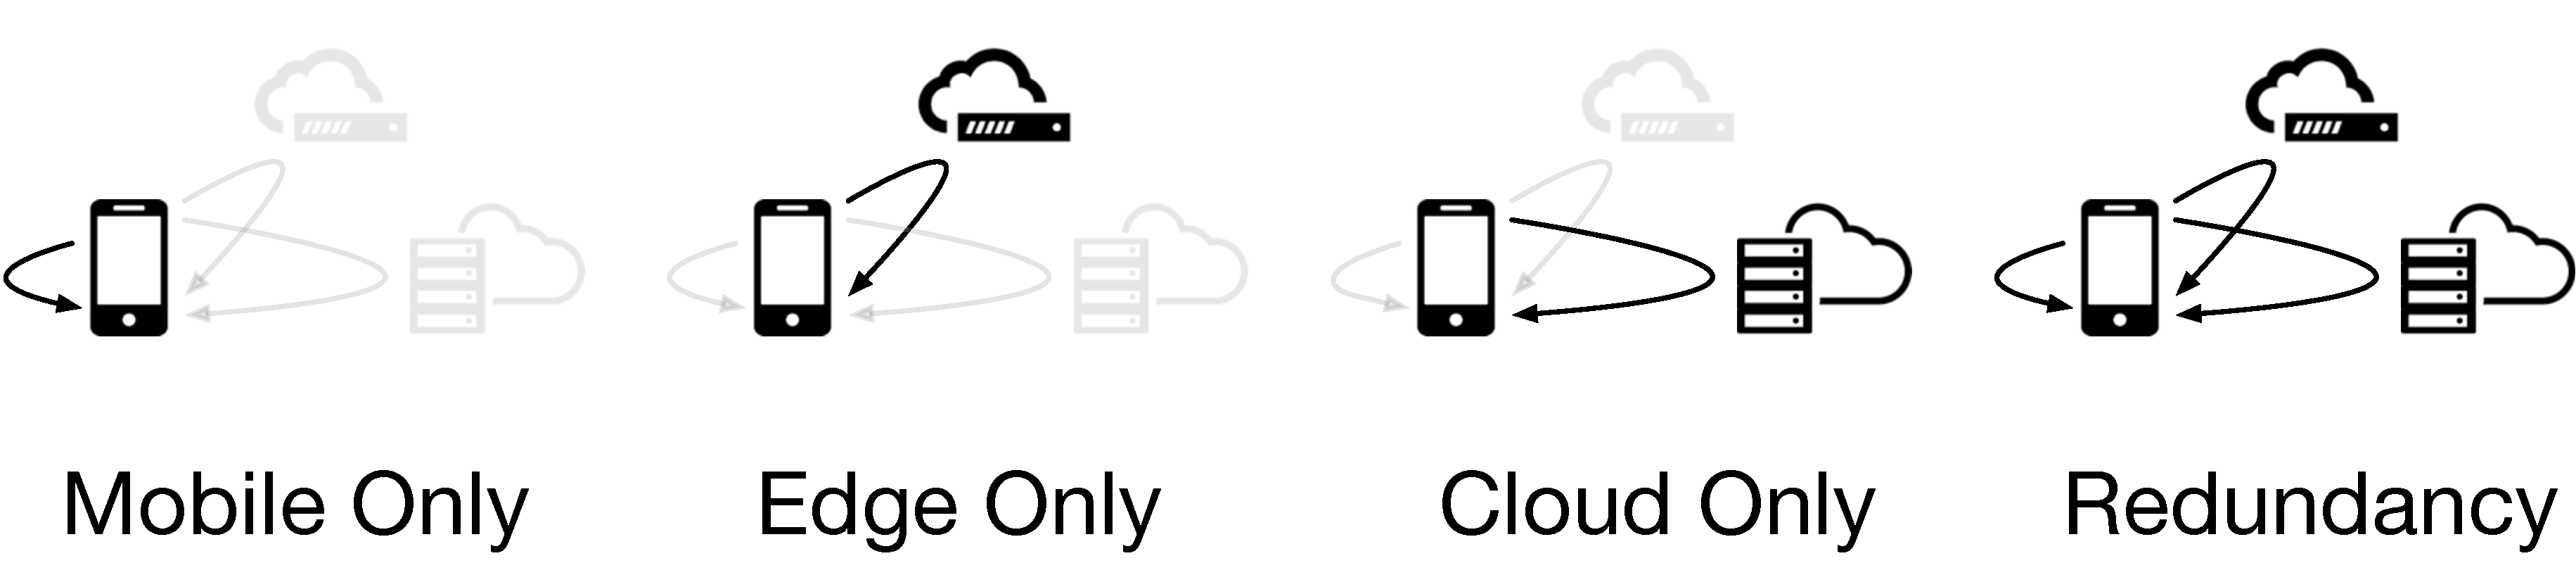
\includegraphics[width=\columnwidth]{figures/redundancy.pdf}
%   \caption{Redundant requests in \sysname{}}
%   \label{fig:redundant}
% \end{figure}

\begin{table*}
  \centering
  \begin{tabular}{c c c c c c}
    \toprule
    Task          & RPi              & Mac             & Swarmbox        & Workstation    & GPU \\
    \midrule
    Encode (JPEG) & 19.6 $\pm$ 2.6   & 4.3 $\pm$ 1.0   & 5.2 $\pm$ 0.9   & 1.3 $\pm$ 0.3  & -   \\
    Decode (JPEG) & 5.4 $\pm$ 0.9    & 1.0 $\pm$ 0.3   & 0.9 $\pm$ 0.2   & 0.5 $\pm$ 0.3  & -   \\
    Viola Jones   & 343.4 $\pm$ 69.4 & 40.0 $\pm$ 10.7 & 48.2 $\pm$ 10.6 & 26.4 $\pm$ 5.7 &     \\
    \bottomrule
  \end{tabular}
  \caption{Performance of analytics operations (serialization, deserialization,
    network transmit, server processing).}
  \label{tab:perf-motiv}
\end{table*}

Our target application environment consists of machines with large range of
computing resources. $(i)$ End-devices, like mobile phones or IoT platforms, are
significantly limited in their computing power. Performing ML inference often
take seconds to complete. $(ii)$ Edge and Cloud. Both the edge and the cloud
suffers from variable latency, unstable connection, and service contention to
provide consistent response times, especially for 99\% requests.

There is a dizzying array of platforms ranging from \$5 Raspberry Pi to \$1000+
GPU-powered workstation~\cite{zhang2015cloud}.  Even in the cloud, there are
various VM options in the cloud: companies rent VMs based on budget or because
of a lack of expertise.

\textbf{Solution:} Because of the such heterogeneity, we hypothesis an ensemble
of available resources (\autoref{fig:dr}) can overcome the shortcomings of
individual platforms and offer end-users with bounded response times, similar to
prior solutions in both cloud-offloading (Tango~\cite{gordon2015accelerating})
and straggler mitigation in the cloud
(Dolly~\cite{ananthanarayanan2013effective}).

\subsubsection*{Network Variations}

\begin{figure}[t]
  \begin{subfigure}[t]{0.49\columnwidth}
    \centering
    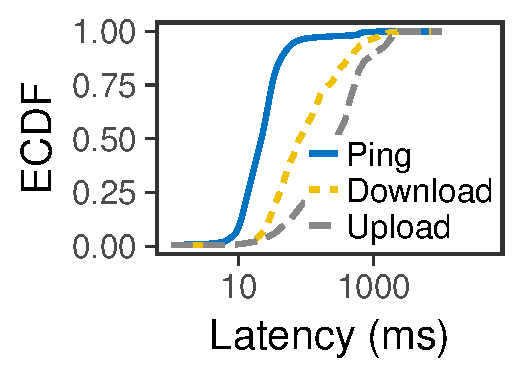
\includegraphics[width=\textwidth]{figures/fcc_latency.pdf}
    \caption{Network latency variation.}
    \label{fig:fcc-latency}
  \end{subfigure}
  \hfill
  \begin{subfigure}[t]{0.49\columnwidth}
    \centering
    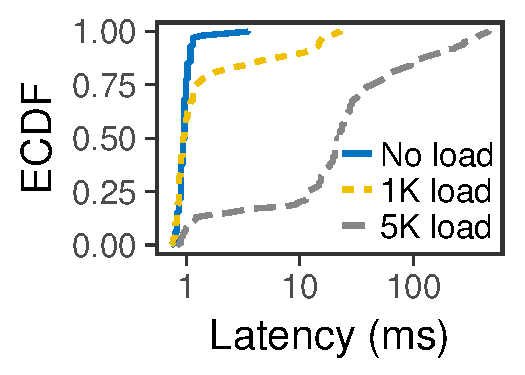
\includegraphics[width=\textwidth]{figures/tf_latency.pdf}
    \caption{Service latency variation.}
    \label{fig:tf-latency}
  \end{subfigure}
  \caption{Network latency increases during downstream and upstream speed tests
    (left). Service time increases during load increase (right).}
\end{figure}

Using FCC broadband measurements, we validate the large variation in wide area
network~(\autoref{fig:fcc-latency}). The median network delay increases from
\SI{22}{\ms} to \SI{80}{\ms} under downstream load and \SI{272}{\ms} under
upstream load.

\textbf{Solution:} Client side, redundant as described above. Server side, time
synchronization and update SLO; and early rejection.

\subsubsection*{Service/Workload Variation}

\noindent We measure TensorFlow serving's performance with different level of load and
validate the large variation in prediction serving
systems~(\autoref{fig:tf-latency}). With modest 1K load, the p99.9 latency
increases from \SI{3.5}{\ms} to \SI{22.5}{\ms}. With 5K load, even the median
latency increases to \SI{21.5}{\ms}: a 22.4$\times$ increase from \SI{0.96}{\ms}
with no load.

\textbf{Solution:} SLO-aware scheduling and the ability to reject requests.

\subsubsection*{Complex Performance Model}

\begin{figure}[t]
  \centering
  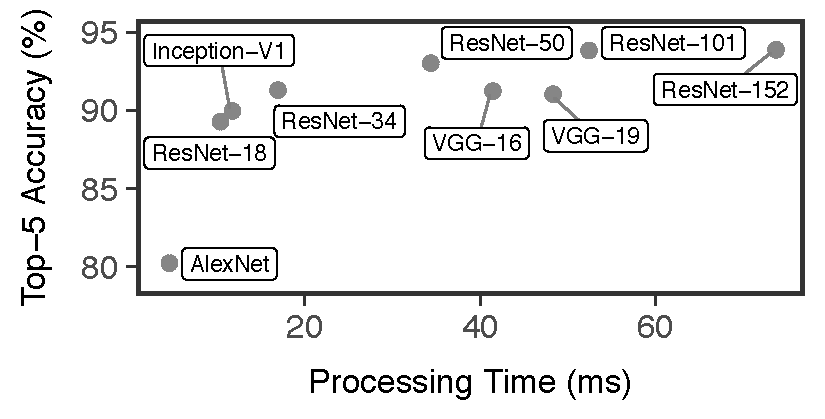
\includegraphics[width=.9\columnwidth]{figures/tradeoff-cnn.pdf}
  \caption{Accuracy-cost trade-off for different CNNs.}
  \label{fig:tradeoff-cnn}
\end{figure}

\begin{figure}[t]
  \centering
  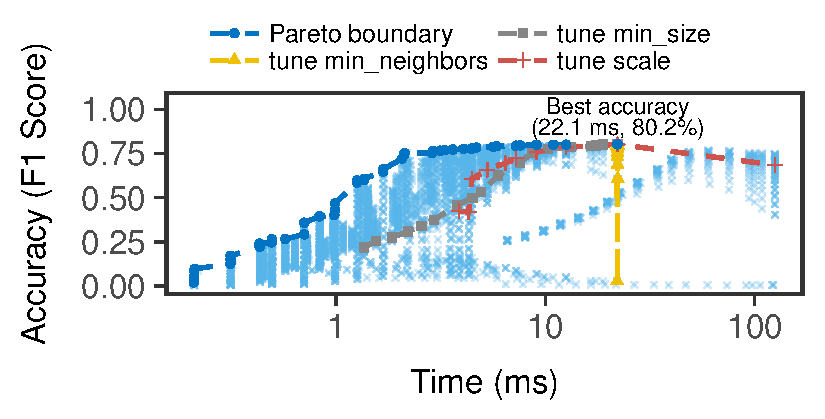
\includegraphics[width=.9\columnwidth]{figures/exhaustive-face.pdf}
  \caption{Complex performance model: spanning multiple dimensions and
    exhibiting non-linear relationship.}
  \label{fig:complex-perf-model}
\end{figure}

For many ML inference task, there exist more than one algorithm, or tunable
parameters for each algorithm with different accuracy and processing times.  We
can speed up computation by providing a less accurate response. This would allow
some computation tractable on end devices and handling more requests on the
edge/cloud.

For example, accuracy-cost trade-offs for object detection using convolutional
neural network (CNN)~\cite{huang2016speed}. \autoref{fig:tradeoff-cnn} shows one
such benchmark~\cite{cnn.benchmarks}.

Many algorithms have large number of knobs to tune that will affect accuracy and
processing cost. We use Viola-Jones (VJ) cascade face
detector~\cite{viola2001rapid} as an example. \autoref{fig:complex-perf-model}
shows the large parameter space with respect to three parameters:
\texttt{min\_size}, \texttt{min\_neighbors}, and \texttt{scale}.

ML algorithms have many tunable parameters. For many algorithms, processing
times and the accuracy may exhibit \textit{non-linear} behavior with respect to
the parameters.

\textbf{Solution:} Bayesian Optimization.

% \begin{table}
%   \small
%   \centering
%   \begin{tabular}{c c c c}
%       \toprule
%       Algorithm & Mobile & Server & GPU \\
%       \midrule
%       VJ Face & $2263.71$ & $197.77 \pm 10.56$ & $23.44 \pm 5.23$ \\
%       HOG + SVM & 1987.9 & 59.7 & 20 \\
%       CNN & $800$ & $300$ & $40$ \\
%       \bottomrule
%     \end{tabular}
%    \caption{Processing Times for Example Model Serving on different
%      platforms.\protect\footnotemark}
%    \label{tab:times}
% \end{table}

% \footnotetext{Mobile is Android Nexus 7; Server is Intel Core XXX; GPU is GTX
%   970. Data is averaged over 100 frames with resolution $640 \times 480$.}

%%% Local Variables:
%%% mode: latex
%%% TeX-master: "../serving"
%%% End:
\section{System Architecture}
\label{sec:sysname-design}

\begin{figure}
  \centering
  \begin{subfigure}[t]{0.9\columnwidth}
    \centering
    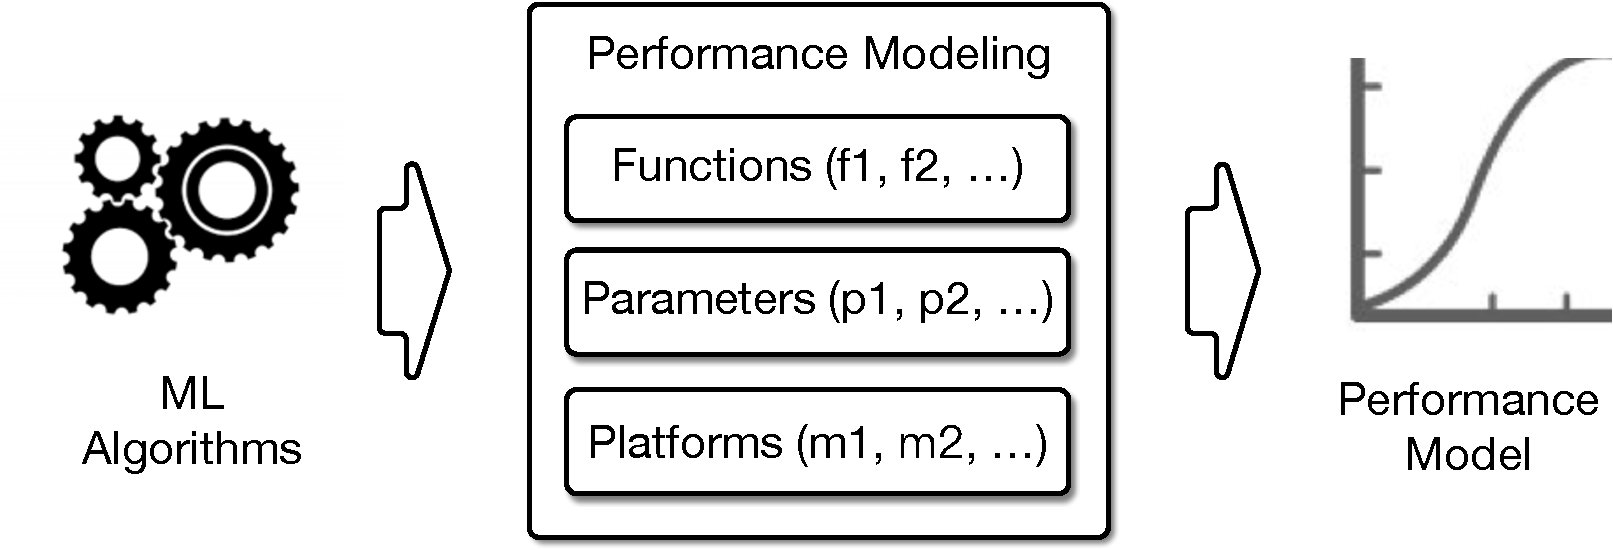
\includegraphics[width=0.9\columnwidth]{figures/offline.pdf}
    \caption{Performance modeling.}
  \end{subfigure}
  \\
  \vspace{1em}
  \begin{subfigure}[t]{0.8\columnwidth}
    \centering
    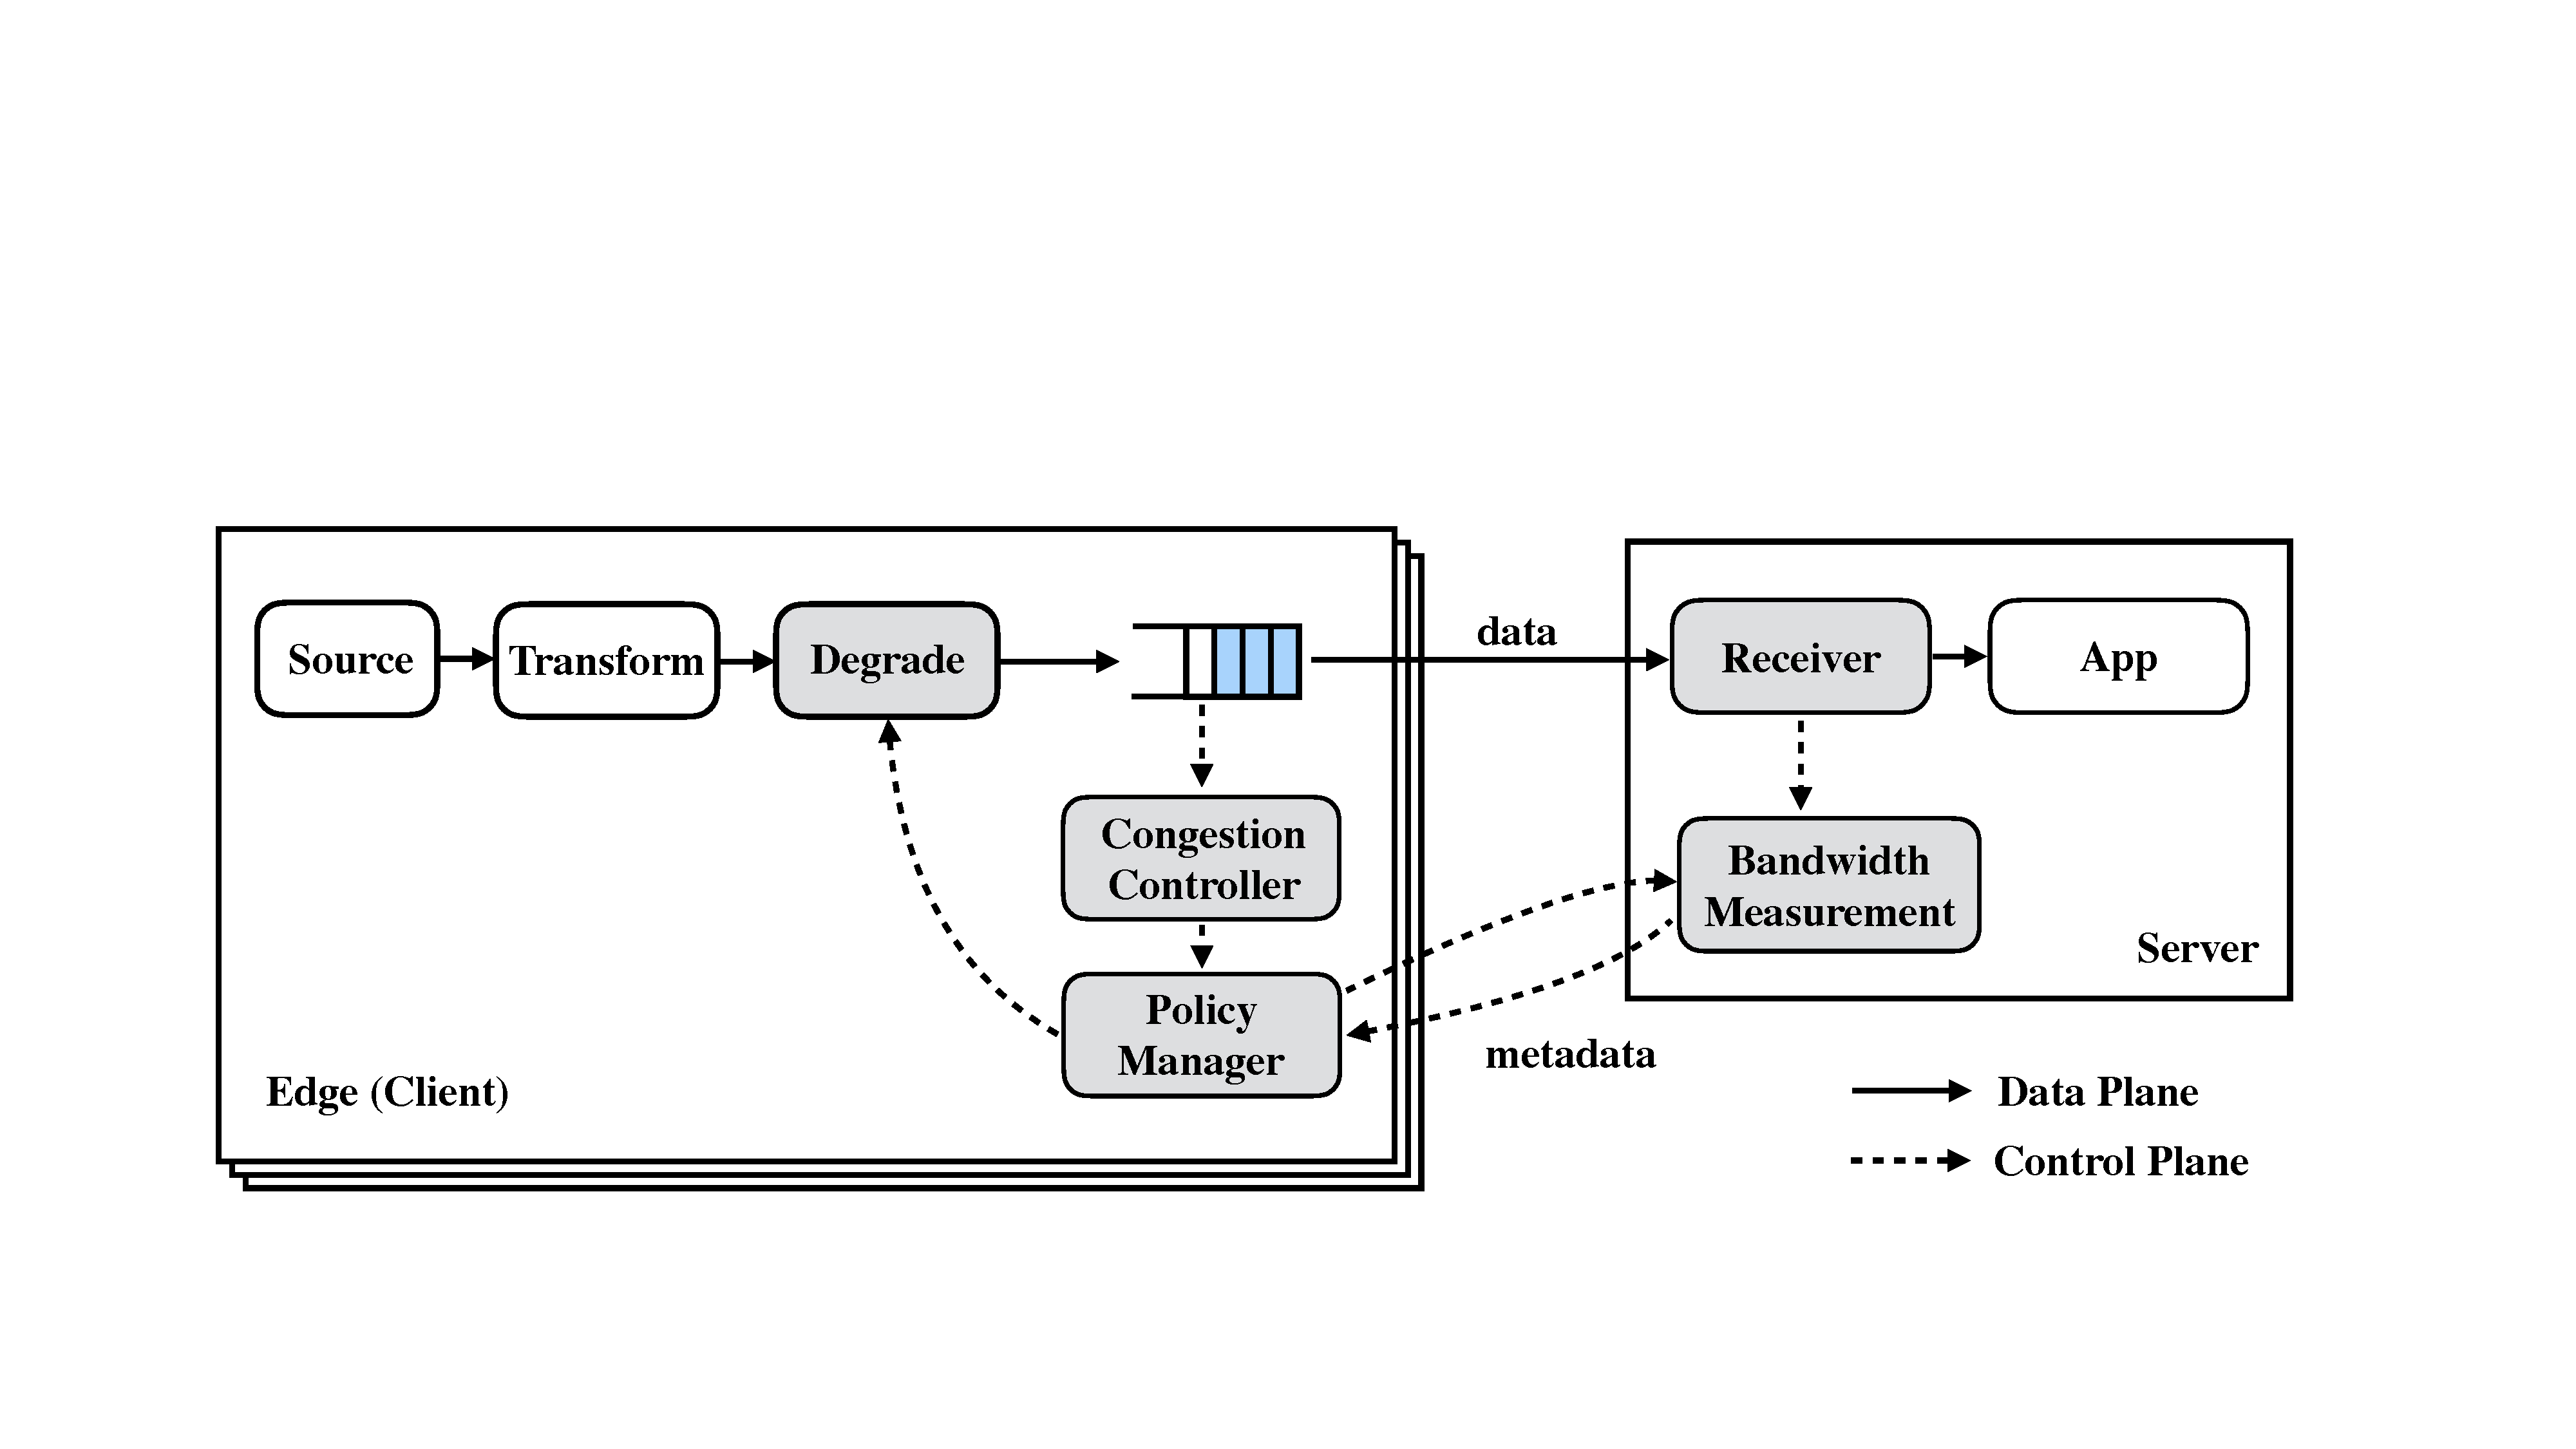
\includegraphics[width=\columnwidth]{figures/runtime.pdf}
    \caption{Runtime dispatch and service triage.}
  \end{subfigure}%
  \caption{\sysname{} Architecture.}
  \label{fig:system}
\end{figure}

We design \sysname{} to address the aforementioned challenges. The architecture
involves two part: performance modelling and runtime serving
(\autoref{fig:system}). \sysname{} integrates multi-objective optimization (MOO)
using Bayesian method to generate the Pareto-optimal set of configurations. To
transfer models across platforms, \sysname{} uses learned performance model as
\textit{a prior} and performs additional sampling if necessary. The client
dispatches requests using multi-armed bandit. The server performs continuous
triage and fast rejects if it cannot meet SLOs.

Before we dive into \sysname{}, we first present the application interface.

Developers don't need to care where exactly a particular function or service is
hosted, as long as it provides the desired output. We abstract the model serving
as a \texttt{predict} API similar to remote procedure call (RPC) interfaces.

\begin{lstlisting}
    predict(input: Input, p: SLA) -> Output
\end{lstlisting}

Internally, the return value is a tuple

\begin{lstlisting}
    Vec<(O: Output, t: Time, a:  Accuracy)>
\end{lstlisting}

\textbf{More to expand here.}

\textbf{How to configure trade-off.}

\section{Performance Modeling}
\label{sec:performance-modeling}

The first step towards bounded response times is to model the relationship
between accuracy and execution time. We then describe the formalism and our
data-driven approach.

\subsection{Problem Formulation}
\label{sec:problem-formulation}

We assume there are multiple algorithms $\mathbb{A}$ available to provide the
same inference. For each algorithm $a \in \mathbb{A}$, it has parameters tunable
to affect processing time $t$ and inference accuracy (or utility $u$). These
parameters could be related to data, such as lowering the image resolution, or
related to the algorithm, such as increasing the scaling factor in HOG. One
instance of the parameters forms a configuration
$\vec{c} = (k_1, k_2, \dots, k_n)$ with $n$ dimensions---we explicitly use the
arrow head here to emphasize configurations' high dimensionality. Running the
algorithm $a$ with a configuration $\vec{c}$ on a machine $m$ yields an
inference with utility $u$ and processing time $t$.

We denote this performance model as a mapping:

{\small \vspace{-1em}
  \begin{equation*}
f: (\mathbb{A} \times \mathbb{C} \times \mathbb{M}) \rightarrow
(\mathbb{R}\times \mathbb{R})
\end{equation*}
} where $\mathbb{A}$ is the set of all algorithms, $\mathbb{C}$ is the set of
all possible configurations, and $\mathbb{M}$ is the set of all machines. The
mapping returns two real values: execution time $t \in \mathbb{R}$ and utility
$u \in \mathbb{R}$. For convenience, we use $\vec{x}$ for the tuple $(a, c, m)$.
Also we use $f_t$ and $f_u$ for the mapping from variables to time $t$ and
utility $u$, respectively.

Bounding the response times is trivial if application accuracy can be
arbitrarily low. \sysname{} aims to minimize response times while maximizing
achievable accuracy---solving a multi-objective optimization problem,
specifically two objectives. For these problems in general, there is no single
optimal solution that jointly minimizes multiple objectives. Instead, there is a
collection of optimal solutions where for any solution, no objective can be
improved without damaging one of the other objectives. The goal of our
performance modeling is to derive such Pareto-optimal
set~\cite{collette2013multiobjective} across all possible
configurations. Formally, the Pareto-optimal set is defined as follows,

{\small \vspace{-1.2em}
  \begin{equation}
    \mathbb{P} = \{ \vec{x} \in \mathbb{X} : \{ \vec{x'} \in \mathbb{X}:
    f_t(\vec{x'}) < f_t(\vec{x}), f_u(\vec{x'}) > f_u(\vec{x}) \} = \varnothing\}
  \label{eq:pareto}
\end{equation}
\vspace{-1.2em}
}

\para{Challenge.} The Pareto-optimal set is easy if we know the mapping for all
possible arguments. However, in practice, the argument space is prohibitively
large, especially for configurations $\vec{c}$ that have many tunable
parameters. It is expensive to run all combinations. Besides, it is also
impossible because developers may not have target machines available.

\para{Solution Overview.} We tackle each dimension differently. For algorithms,
because their differences are substantial, our profiler evaluates all available
algorithms exhaustively. For each algorithm, to address the curse of
dimensionality of $\vec{c}$, we use BO to reduce space search and only find
near-optimal $c$s. For different machine $m$, because only $f_t$ depends on $p$,
we show that the Pareto-optimal set doesn't change if the execution time $f_t$
satisfies monotonicity. We approximate $f_t$ with a simple linear model.

\subsection{Composing Algorithms}
\label{sec:compose-models}

There are different algorithms. Different implementation for GPU and CPU.

We have to profile each individual algorithm.

Observation: their profile (the Pareto-optimal set) are composable by merge and
compare all of them.

\subsection{Modeling Parameters}
\label{sec:single-platform}

Evaluating all configurations across the large parameter space is prohibitively
expensive. To reduce the number of samples we need, \sysname{} builds a
performance model that is just accurate enough to allow us to distinguish
near-optimal configurations from the rest. This is similar to recent systems,
such as CherryPick~\cite{alipourfard2017cherrypick} and
BOAT~\cite{dalibard2017boat}, that use Bayesian optimization (BO) to improve
performance across a large number of configurations.

While previous approaches often transform the multi-objective problem into a
single-objective problem using scalarization techniques (an approach that is
expected to be suboptimal~\cite{knowles2006parego}.) We adopted the
PESMO~\cite{hernandez2016predictive}, which does not transform the
multi-objective problem into a single-objective. PESMO also has a low
computational cost. It grows linearly with respective to the total number of
objectives $K$.

\subsection{Modeling Machines}
\label{sec:performance-transfer}

We make the observation that $f_u(a, c, m)$ doesn't depend on $m$. If we assume
a monitonicity between $f_t(m_1)$ and $f_t(m_2)$, we can prove that the
Pareto-set is directly transferable. The monitonicity is a condition that if on
one platform it takes longer for one configuration,
i.e.\,$f_t(a, \vec{c}, m_1) < f_t(a, \vec{c'}, m_1)$, then it will take longer
on another platform, i.e.\,$f_t(a, \vec{c}, m_2) < f_t(a, \vec{c'}, m_2)$.

Based on these two assumption, one can prove that if $\vec{x}_i$ is in the
Pareto-optimal set $\mathbb{P}_1$ for platform $p_1$, then $\vec{x}_i$ will also
be in the Pareto-optimal set $\mathbb{P}_2$. And the profile on $p_2$ will be a
stretched or shrunk version for $p_1$ along the time dimension.

This simplifies our model transfer across platforms and makes it possible to
derive the performance model at runtime by sampling only a few performance
measures. In practice, a simple linear transformation suffices in giving a
reasonably precise transfer.

\section{Runtime System}
\label{sec:runtime-system}

\subsection{Client Dispatch}

The decision layer dispatches the requests to multiple instance of servers. The
decision is based on the service level aggreement (SLA) that developer
specficies. After servers complete the inference, results are returned and
merged. The merging process is similar to the \texttt{Reduce} phase in MapReduce
that combines the vector of return values into a single response. We provide a
few different merging policies corresponding to different SLAs:

\para{Earliest first}. For all running services, the earliest return will be
used first. When the user specifices SLA with minimal response time, policy
achieves the minimal possible response times.

\para{Eventual accurate}. For return type such as a set, the merge can be
automatically done by combining the individual results. In this way, the system
may return a less accurate result first for timeliness, but eventually, the
system will yield a higher accuracy. This requires either the return type
implements \texttt{Merge} interface. For common data types such as \texttt{Set}
or \texttt{List}, we've implemented the interface for developers. For advanced
types, as we will demonstrate in the image example, developers can implement
this interface by themselves.

\para{Bounded time}. With a configured time bound, \sysname{} will pick the
results with the highest accuracy that are within the deadline.

\para{Bounded accuracy}. With a configured lower bound on the accuracy,
\sysname{} will pick the results with the smallest response times.

At runtime, \sysname{} dispatches application request to multiple platforms and
combine their results transparently. It makes the decision of where to run (what
platform to use) and how to run (what configuration to use) to satisfy
application requirement. The decision is related with the desired guarantee the
developer has expressed using our API and the condition during the application
execution.

\para{Static scheduling.} Our baseline schedule makes decision based on an
estimation of the network latency and server response time. If the algorithm can
be executed locally, it will do. If the algorithm cannot run locally in full
accuracy, we shall do it locally, together with offloading requests to available
servers.

\para{Statistical scheduling.} We cast the dispatch as a multi-armed bandit
problem. Different from existing approaches where pulling each arm doesn't incur
much cost; in our settings, local processing and remote communication has an
associated cost. This is multi-armed bandit with budget.

\subsection{Server Calibration}

Calibrate the profile by running.

\subsection{Server Scheduling}
\label{sec:server-scheduling}

The server runs a novel real-time scheduling algorithm that maximizes the
throughput and achievable accuracy while meeting SLOs. \sysname{} employs a fast
reject if serving the new request will violate the SLOs of any pending
requests. By rejecting instead of queuing up, \sysname{} addresses server
contention and reduces tail latency even under contention.

Rejection must be a cheap operation to sustain large number of concurrent
requests. In \sysname{}, we maintain a variable \texttt{capacity} that is
updated whenever a worker thread starts or finishes serving. Determining
schedulability is essentially comparing the request's SLO with available
capacity.

\para{Scheduling}. Given each task with a deadline constrain and the degree of
freedom of trading off quality for processing times, the scheduler finds the
best scheduling strategy.

\para{Acceptance test}. Perform admission control at the arrival of requests to
verify the schedulability of the task set. If the task set is found schedulable,
the new task is accepted in the system; otherwise, it is rejected.

\para{Re-scheduling}. A naive scheduler will either always run at highest
quality with lowest throughput; or lowest quality with highest throughput. A
better scheduler that explores the trade-off but with a naive design will
perform re-scheduling at every job arrival. The desired scheduler only
re-schedules when necessary.

%%% Local Variables:
%%% mode: latex
%%% TeX-master: "../serving"
%%% End:

%% LocalWords: schedulability
\newpage

\section{Implementation}
\label{sec:implementation}

We implement BO-based performance modeling with Spearmint package. Our runtime
client and server communicate through an RPC interface. Currently, we have
implemented face detection, pedestrian detection, and object detection.

\begin{table}
  \footnotesize
  \centering
  \begin{tabular}{c c c c}
    \toprule
    Application & Algorithms & Dataset \\
    \midrule
    Face & Viola-Jones, LBP & FDDB \\
    \midrule
    Object & ResNet, Inception, AlexNet & ImageNet \\
    \bottomrule
  \end{tabular}
  \caption{\sysname{} Applications}
  \label{tab:apps}
\end{table}

\newpage

Details about how we implement the applications.

\newpage

%%% Local Variables:
%%% mode: latex
%%% TeX-master: "../serving"
%%% End:

\newpage

\section{Related Work}
\label{sec:related-work}

\para{Model Serving.} Frameworks such as Clipper~\cite{crankshaw2017clipper} and
TensorFlow Serving~\cite{tensorflow2017serving} only focus on system-level
techniques such as batching and hardware acceleration to improve
throughput. While Clipper allows ensemble of models, the purpose is to improve
accuracy at the cost of resources. Both frameworks have poor performance when
under overload.

\para{Mobile-Cloud Offloading.} Prior offloading framework, such as
MAUI~\cite{cuervo2010maui}, CloneCloud~\cite{chun2011clonecloud},
Gabriel~\cite{ha2014towards}, and Tango~\cite{gordon2015accelerating}, runs the
same algorithm (with the same configurations) across different machines: a poor
match for the future heterogeneous mobile-edge-cloud (MEC)
environment. \sysname{} explicitly models performance and select the appropriate
algorithm and configuration at runtime.

\para{Low Latency via Redundancy.} The idea of initiating redundant operations
across diverse resources and using the first result which completes has been
explored in many contexts, such as cloud
computing~\cite{ananthanarayanan2013effective}, cloud
service~\cite{dean2013tail}, wide-area network service~\cite{vulimiri2013low},
and mobile applications~\cite{gordon2015accelerating}. We extends the redundancy
and offer a variety of policies for combining results from multiple services.

\para{Approximate Techniques.} With the increasing workload to handle, recent
systems~\cite{agarwal2013blinkdb, rabkin2014aggregation, zhang2017live}
recognizes that timely-despite-inaccurate results are better than late
results.

\para{Bayesian Optimization.} To optimize complex systems in a principled way,
many frameworks employ Bayesian Optimizations to tune application behavior, such
as CherryPick~\cite{alipourfard2017cherrypick}, FLASH~\cite{zhang2016flash}, and
BOAT~\cite{dalibard2017boat}. These frameworks focus on single-objective
optimization: minimizing job completion time or maximizing application
accuracy. In contrast, \sysname{} addresses a multi-dimensional optimization
between application accuracy and processing times. We demonstrated that BO
outperforms greedy heuristic approach used in VideoStorm~\cite{zhang2017live}.

\para{SLO-awareness.} MittOS~\cite{hao2017mittos} advocates the return of
\texttt{EBUSY} for IO operations to bound IO requests.

%%% Local Variables:
%%% mode: latex
%%% TeX-master: "../serving"
%%% End:

\section{Evaluation}
\label{sec:evaluation}

In this section, we provide evaluation results for \sysname{}:

\begin{itemize}[itemsep=0pt, topsep=1pt]
\item[\autoref{sec:perf-modeling}] Compared with naive approaches (random and
  gradient-based search), \sysname{} finds a Pareto front that is closer to the
  optimal (\autoref{fig:bo}).
\item[\autoref{sec:runtime}] For all applications, \sysname{} achieves bounded
  service latency across various network conditions (\autoref{fig:end-to-end}).
\end{itemize}

\subsection{Performance Modeling}
\label{sec:perf-modeling}

This section shows that BO can effectively explore the large design space and
come up with a better Pareto-optimal parameter set. We compare \sysname{} with
two baseline profilers: $(i)$ greedy approach as described in
VideoStorm~\cite{zhang2017live}; $(ii)$ random sampling.

Greedy converts MOO into SOO with a parameter $X = \beta$ $A - \beta T$. It
starts with a random configuration $c$ and then picks a neighbor configuration
(by changing the value of a random dimension). If the new configuration $c'$
returns a higher $X$, it updates and iterate form $c'$ again. Otherwise, it
picks a different neighbor $c''$ by changing another dimension. It starts with
three random starting point; it also evaluate a number of random $\beta$.

\autoref{fig:bo} shows that with the same budget (the number of parameters to
evaluate), our profiler can find parameters with better trade-offs between
application accuracy and processing times.

\begin{figure}
  \centering
  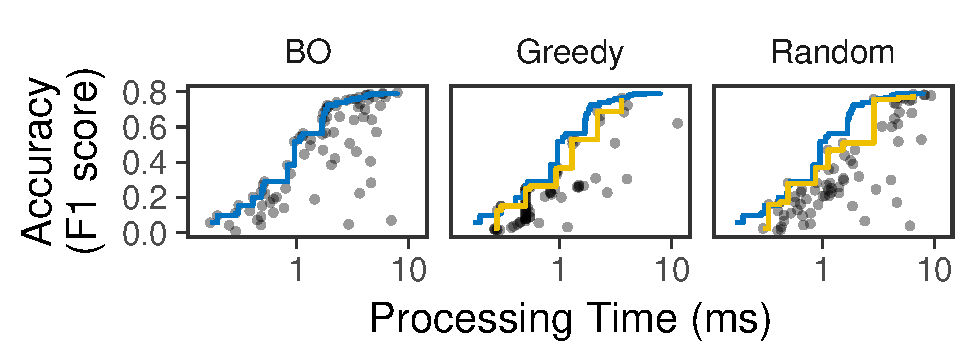
\includegraphics[width=0.95\columnwidth]{figures/profiling.pdf}
  \caption{Using Face as an example, BO evaluates 50 configurations and
    recommends 29 configurations as the Pareto-optimal boundary (the blue
    line). Greedy and Random find sub-optimal Pareto configurations with a
    budget of 80 evaluations (the yellow line in each figure).}
  \label{fig:bo}
\end{figure}

\newpage

\subsection{Runtime Evaluation}
\label{sec:runtime}

To make \sysname{} story compelling, we are convincing the readers the following
points:

\begin{enumerate}[leftmargin=*, itemsep=5pt]
\item Heavy computations are beyond the capabilities of end devices. (Face
  Detection on RPi takes 327 ms). While on a modest workstation, only 27 ms.
\item Naively offloading computation to the cloud does not offers bounded
  response times. Show time series or statistics by injecting traffic or
  additional workload.
\item One can use edge computing, but it is not clear what edge devices are
  capable.
\item To effectively utilizing available resources, cloning can help. Cloning
  without adaptation is not useful on low end devices.
\item Cloning with performance modeling improves.
\item Cloning with performance modeling and server rejection (SLO-awareness)
  improve further.
\end{enumerate}

Point 1, 2, 3 should have been shown in intro and motivation. We only show their
numbers here as reference lines in figures. The runtime experiment is mainly
focusing on demonstrating point 4/5/6, that is, how effective are differential
redundancy and server triage.

\textbf{Methodology:} RPi as the end device, modest server as edge (with and
without GPU), and Amazon EC2 as server (with GPU). RPi and the edge exist within
the same network (~1-2 ms latency).

\begin{figure}
  \centering
  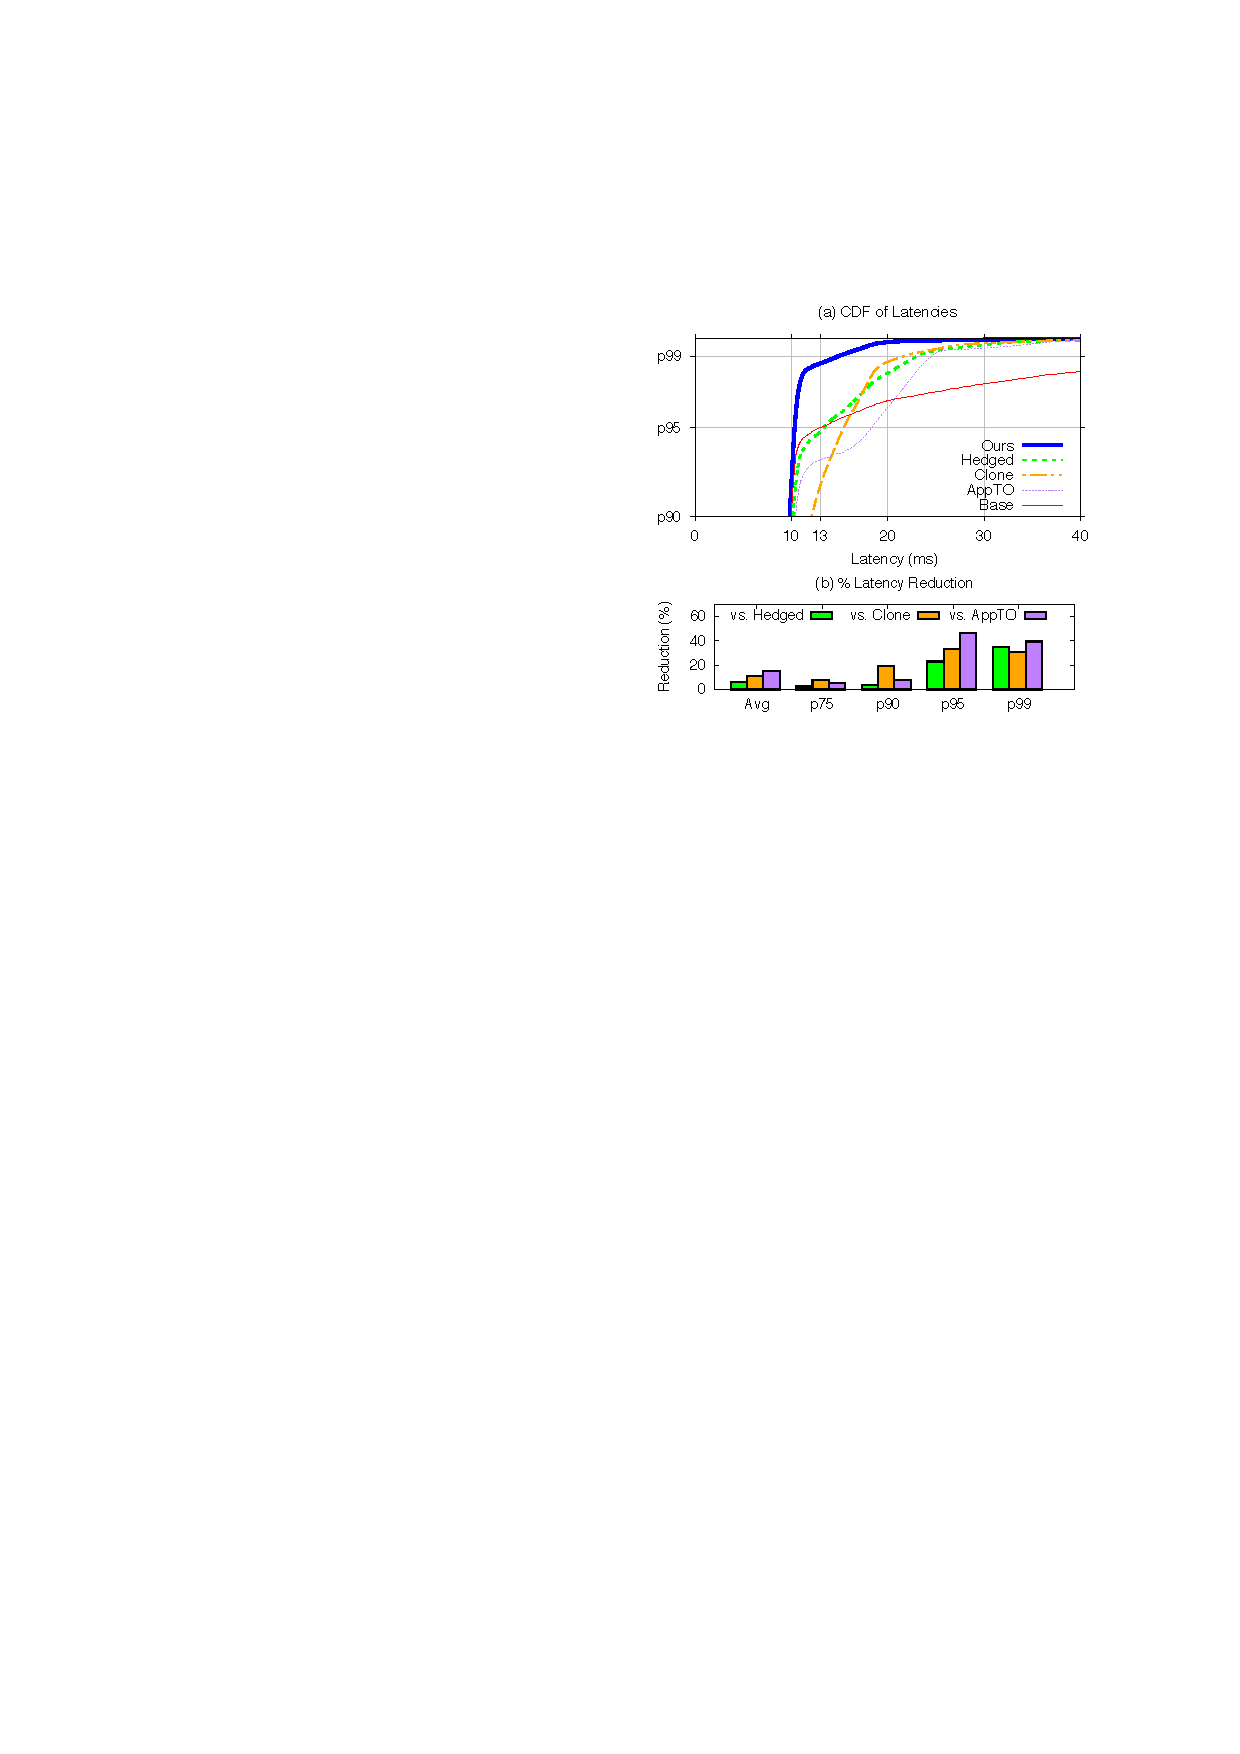
\includegraphics[width=0.95\columnwidth]{figures/runtime-mock.pdf}
  \caption{Compared with other techniques used in reducing tail latency,
    \sysname{} is able to maintain a lower latency bound.}
  \label{fig:eval-runtime}
\end{figure}

\begin{figure}
  \centering
  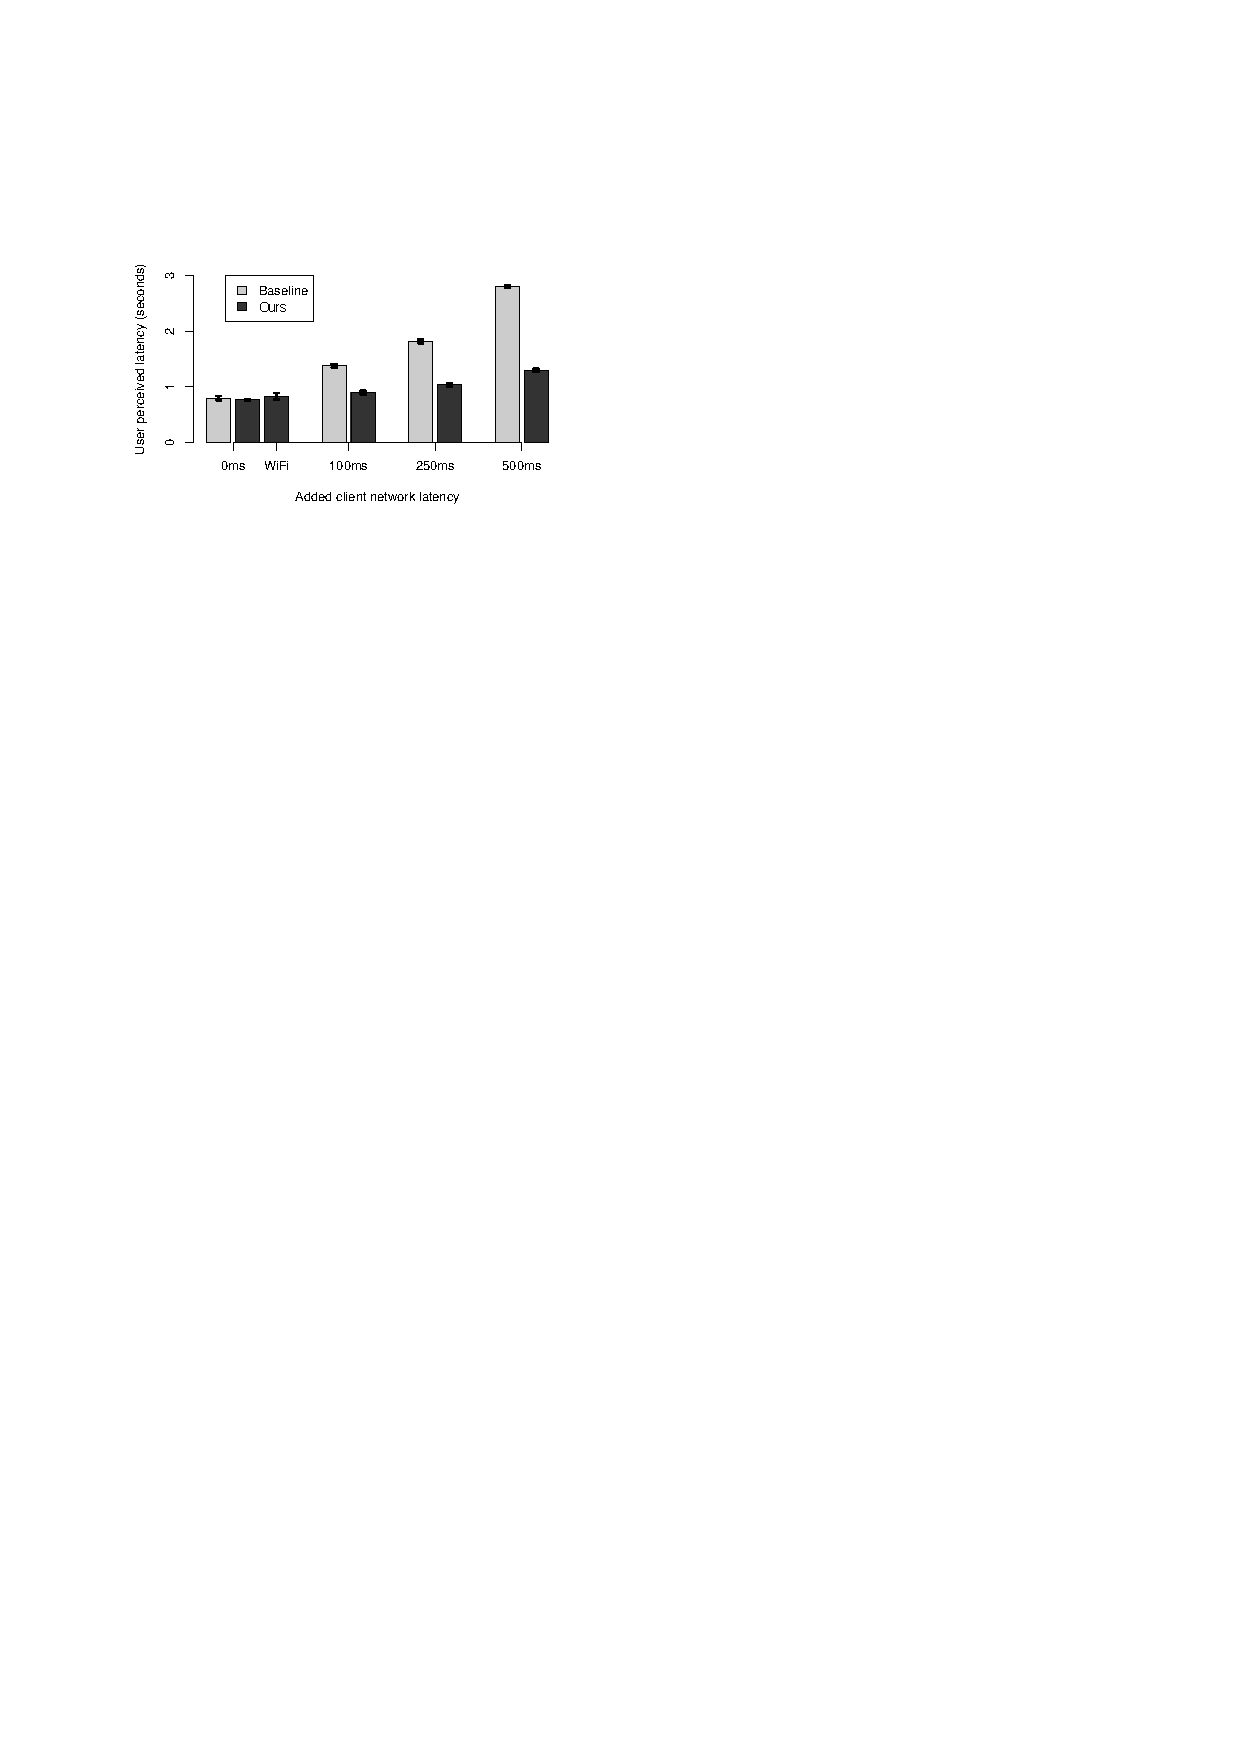
\includegraphics[width=0.95\columnwidth]{figures/eval-net-conditions.pdf}
  \caption{Under different network conditions, \sysname{} maintains bounded
    response times.}
  \label{fig:end-to-end}
\end{figure}

\newpage

Edge computing promises closer resources to end devices, offering better
response time guarantees. While edge servers can be orders-of-magnitude more
powerful than mobile devices, its capability may be limited by budget. We
evaluate the performance \sysname{} with different capabilities of the edge
(with and without GPU).

\subsection*{Serving Overhead}
\label{sec:serving-overhead}

To evaluate our technique against workload variation, we compare \sysname{} with
TensorFlow Serving (TFS), the state-of-the-art framework for deep
learning. While TFS supports loading and serving multiple models, it is more
designed for multiple versions of the same model (in the scenario of A/B
testing). For our evaluation, we only compare us against TFS with one model. The
evaluation is also limited to Object, because TFS is designed for DL
applications and integrating OpenCV algorithms would take too much time for
little purpose. The goal here is to show that \sysname{} adds little overhead
under normal conditions (performance on par with TFS) and is able to adapt and
maintain SLO during service contention (better tail performance).


\newpage

%%% Local Variables:
%%% mode: latex
%%% TeX-master: "../serving"
%%% End:

\section{Limitations and Future Work}
\label{sec:limitations}

Discuss implementation limitations.

\newpage

%%% Local Variables:
%%% mode: latex
%%% TeX-master: "../../thesis"
%%% End:

\section{Conclusion}
\label{sec:conclusion}

In this paper, we present \sysname{} that allows bounded response times for wide
area prediction serving.

One can view our approach as an extended version of the original ``CAP''
theorem. Consistency, as a form of correctness, is relaxed to be accuracy
ranging from 0 to 1. Availability is relaxed to be the response times. Under
network partition, traditional systems choose either consistency or
availability. In \sysname{}, we explore the direction of maximizing application
accuracy (correctness) with given availability guarantee.

Two more paragraph.

%%% Local Variables:
%%% mode: latex
%%% TeX-master: "../serving"
%%% End:

%%% Local Variables:
%%% mode: latex
%%% TeX-master: "../thesis"
%%% End:

%%% Local Variables:
%%% mode: latex
%%% TeX-master: "../thesis"
%%% End:

% \chapter{Conclusion and Future Work}
\label{cha:concl-future-work}

Conclusion here.

%%% Local Variables:
%%% mode: latex
%%% TeX-master: "../thesis"
%%% End:


\printbibliography

\end{document}
